\ctexset{
chapter/name = {\S,},
chapter/number = \arabic{chapter},
section/number = {\arabic{chapter}.\arabic{section}},
}

\part[2014日萌全程回顾]{{\sffamily\hei {\rm\toppanb アニメ最萌トーナメント}\\{\rm\toppanb 2014}日萌\\全程回顾}\\[5em]
\begin{center}
 \zihao{4}\rm\kasho {王者自由}
\end{center}}
\setcounter{chapter}{0}

首先纪念在今年度萌、日萌、世萌、新星萌等萌战战场上战斗过和正在战斗中的角色和作品,不管你们的战绩如何,都诠释了自己的萌;

也希望那些坚持不懈的萌战痴、厨子和刷子们,不要因为萌战胜负失去对角色爱的本心。

\emph{我希望尽量客观地记述2014年日萌的所有我知道的细节,使这些历史不要被遗忘,以及希望以后想成为大厨的以史为鉴。希望读者能够以观众的心态去阅读这份记载。}

海外厨团四家:\uwave{麻将}、\uwave{圆脸}、\uwave{电磁}、\uwave{LL},分别简称为\uwave{麻}、\uwave{圆}、\uwave{电}、\uwave{L}(\uwave{拉});为了与魔炮做区分,不再简称\uwave{电磁}为炮。如无特别标明,厨团指的都是海外厨团,大厨也都是海外大厨,这是日萌事实。\uwave{麻将}领袖\uline{自由}、\uwave{圆脸}领袖\uline{兰博}、\uwave{电磁}领袖\uline{小九}、\uwave{LL}领袖\uline{冰凉},以后都以此为代称。

文章的主视角是2014年\uwave{麻将}厨和\uline{东山}厨的\uline{自由},由此产生的价值观偏向是必然的。并且,\uline{自由}有时是\uwave{麻将}厨的立场,有时是\uline{东山}厨的立场,有时是平衡厨的立场,所以当使用\uline{自由}这一代称的时候,并不能单纯地当做\uwave{麻将}领袖。同样对于其他出现的人物,都不能完全代表其阵营。
\\[3em]

值得注意的是,本文写于2014年末和2015年初期间,虽为印刷作了少许版面上的调整,但依然反映的是当年的情况。时过境迁,和现在相差很多的内容,也请代入当时的时代背景,这也正是特定时代的特定产物。

\chapter{预选}

0705提名结束,共计提名约3000人,300多部作品。整理一下提名作品的人数情况,这个实际上可以作为作品阵营势力分布来看,\uwave{麻将}一直占据的人数优势就是从提名开始的。\uwave{Q娃系列}集合5部作品坐居第二,而单作品仅次于\uwave{麻将}的则是卡牌番\uwave{幻想玩偶}。当然前几名多数是幼女向动画也是很正常的。深夜番也有几个人数多的作品,比如\uwave{STB}、\uwave{超炮}、\uwave{LL}。有人猜测\uwave{舰娘}出场会打破这个记录。

\DataTable{提名人数排行}{|cclc|}{\hline
\thead 系列 & \thead 人数 & \thead 名称 &\\\hline
天麻 & 88 & \mincho \Saki &\\\hline
\multirow{5}{*}{光美} & \multirow{5}{*}{64} & \mincho ドキドキ!プリキュア& (20)\\
 & & \mincho ハピネスチャージプリキュア!& (11)\\
 & & \mincho 映画~ドキドキ!プリキュア~マナ結婚!!?未来につなぐ希望のドレス& (2)\\
 & & \mincho 映画~プリキュアオールスターズNewStage3~永遠のともだち& (12)\\
 & & \mincho プリキュアシリーズ& (19)\\\hline
FD & 60 & \mincho ファンタジスタドール&\\\hline
\multirow{2}{*}{美旋} & \multirow{2}{*}{41} & \mincho プリティーリズム·レインボーライブ& (38)\\
 & & \mincho プリティーリズム·オールスターセレクション& (3)\\\hline
偶活 & 35 & \mincho アイカツ!-アイドルカツドウ-&\\\hline
\multirow{2}{*}{im@s} & \multirow{2}{*}{35} & \mincho THE IDOLM@STER MOVIE~輝きの向こう側へ!& (21)\\
 & & \mincho ぷちます!!-プチプチ·アイドルマスター-& (14)\\\hline
萝球 & 32 & \mincho ロウきゅーぶ!SS &\\\hline
宝宠 & 30 & \mincho ジュエルペット~ハッピネス&\\\hline
STB & 30 & \mincho ストライク·ザ·ブラッド &\\\hline
IS & 29 & \mincho IS〈インフィニット·ストラトス〉 2 &\\\hline
电磁 & 29 & \mincho \Railgan &\\\hline
LL & 29 & \mincho ラブライブ! &\\\hline
MH & 28 & \mincho ふたりはミルキィホームズ &\\\hline
人偶 & 28 & \mincho ローゼンメイデン &\\\hline
WUG & 27 & \mincho Wake Up, Girls! &\\\hline
}

\section{07/13(日) 预选分组}

预选的分组还是相对顺畅的,\uwave{圆}\uwave{麻}两个在今年开赛前就定下的大阵营并没有大的冲突。这年的\uwave{麻将}阵营主要参与者,在度萌靠着\uwave{圆脸}大腿内战拿了个四强,虽然连个从者都没有给,不过还是弱鸡的\uwave{麻将},在日萌初期抱紧\uwave{圆脸}大腿显然是最好的选择。

下页的表格实际上是\uwave{麻将}预选决定的弃保。
\\

由于\uwave{麻将}去年的弱势,八强无望的阴影笼罩着\uwave{麻将}阵营,于是本为度萌\uwave{麻将}资金来源的流子打算组建\uwave{LL}的厨团。\uwave{LL}厨团领袖\uline{冰凉}在\uwave{LoveLive吧}发起了招募出团的置顶帖,由此找来了以\uline{梨落}为主的一批萌战老厨,这是后话。

这个是\uwave{LL}预选的分组:

\def\iD{\mincho}
\def\iA{\toppanb\cellcolor{lovelive}}
\def\iB{\toppanb}
{\zihao{6}\mincho\ctexset{space=true}
\begin{longtable}{|rrl|}\hline
E01組 & 7月24日 & \iA 矢澤にこ@ラブライブ!\\
 & & \iA 園田海未@ラブライブ!\\\hline
E02組 & 7月25日 & \iD ことりの母@ラブライブ!\\
 & & \iD 放送部員A@ラブライブ!\\
 & & \iA 高坂穂乃果@ラブライブ!\\
 & & \iB 矢澤ココロ@ラブライブ!\\
 & & \iA 西木野真姫@ラブライブ!\\
 & & \iA 絢瀬絵里@ラブライブ!\\\hline
E03組 & 7月26日 & \iD アナウンサー@ラブライブ!\\
 & & \iD アルパカ@ラブライブ!\\
 & & \iD 放送部員B@ラブライブ!\\
 & & \iB 高坂雪穂@ラブライブ!\\\hline
E04組 & 7月27日 & \iD ミカ@ラブライブ!\\
 & & \iB 優木あんじゅ@ラブライブ!\\\hline
E05組 & 8月3日 & \iD リス@ラブライブ!\\
 & & \iA 南ことり@ラブライブ!\\
 & & \iA 小泉花陽@ラブライブ!\\\hline
E06組 & 8月4日 & \iD フミコ@ラブライブ!\\
 & & \iB 矢澤ココア@ラブライブ!\\
 & & \iB 絢瀬亜里沙@ラブライブ!\\\hline
E07組 & 8月5日 & \iD にこの母@ラブライブ!\\
 & & \iD ヒデコ@ラブライブ!\\
 & & \iB 綺羅ツバサ@ラブライブ!\\
 & & \iA 星空凛@ラブライブ!\\
 & & \iD 真姫の母@ラブライブ!\\\hline
E08組 & 8月6日 & \iA 東條希@ラブライブ!\\
 & & \iD 穂乃果の母@ラブライブ!\\
 & & \iB 統堂英玲奈@ラブライブ!\\
 & & \iD 先生@ラブライブ!\\\hline
\end{longtable}}

\newpage

\def\iD{\mincho}
\def\iA{\toppanb\cellcolor{saki}}
\def\iB{\mincho\cellcolor{saki}}
\def\iC{\toppanb}
\def\SakiZen{@\Saki}
{\zihao{6}\mincho\ctexset{space=true}
\begin{longtable}{|rl||rl|}\hline
\renewcommand{\thefootnote}{\alph{footnote}}
\renewcommand\footnoterule{}
E01組 & \iC 東横桃子\SakiZen & E05組 & \iA エイスリン·ウィッシュアート\footnotemark[2]\\
7月 & \iA 宮永照\SakiZen & 8月 & \iB 薄墨初美\SakiZen\\
24日 & \iA 国広一\SakiZen & 3日 & \iC 加治木ゆみ\SakiZen\\
 & \iC 花田煌\SakiZen & & \iD 津山睦月\SakiZen\\
 & \iD 久保貴子\SakiZen & & \iA 清水谷竜華\SakiZen\\
 & \iD 山谷ひな\SakiZen & & \iD 室橋裕子\SakiZen\\
 & \iD 深堀純代\SakiZen & & \iC 藤原利仙\SakiZen\\
 & \iC 狩宿巴\SakiZen & & \iD 西田順子\SakiZen\\
 & \iD 埴淵久美子\SakiZen & & \iA 小瀬川白望\SakiZen\\ \cline{1-2}
E02組 & \iD 安河内美子\SakiZen & & \iA 新子憧\SakiZen\\
7月 & \iC 本内成香\SakiZen & & \iA 姉帯豊音\SakiZen\\ \cline{3-4}
25日 & \iC 多治比真佑子\SakiZen & E06組 & \iC ネリー·ヴィルサラーゼ\footnotemark[3]\\
 & \iC 福与恒子\SakiZen & 8月 & \iC ハオ慧宇\footnotemark[4]\SakiZen\\
 & \iC 鶴田姫子\SakiZen & 4日 & \iC 赤土晴絵\SakiZen\\
 & \iD 能口彩花\SakiZen & & \iA 福路美穂子\SakiZen\\
 & \iC 野依理沙\SakiZen & & \iA 夢乃マホ\SakiZen\\
 & \iD 佐藤裕子\SakiZen & & \iA 末原恭子\SakiZen\\ \cline{1-2}
E03組 & \iD ギバード桜子\SakiZen & & \iB 瑞原はやり\SakiZen\\
7月 & \iD 赤阪郁乃\SakiZen & & \iC 三尋木咏\SakiZen\\
26日 & \iA 大星淡\SakiZen & & \iA 松実玄\SakiZen\\
 & \iD 伏屋那都\SakiZen & & \iA 天江衣\SakiZen\\
 & \iA 高鴨穏乃\SakiZen & & \iD 文堂星夏\SakiZen\\
 & \iA 宮永咲\SakiZen & & \iD 亦野誠子\SakiZen\\
 & \iD 戒能良子\SakiZen & & \iD 針生えり\SakiZen\\ \cline{3-4}
 & \iC 龍門渕透華\SakiZen & E07組 & \iC メガン·ダヴァン\footnotemark[5]\\
 & \iC 雀明華\SakiZen & 8月 & \iB 白水哩\SakiZen\\
 & \iC 染谷まこ\SakiZen & 6日 & \iC 弘世菫\SakiZen\\
 & \iC 渋谷尭深\SakiZen & & \iC 荒川憩\SakiZen\\
 & \iC 神代小蒔\SakiZen & & \iC 吉留未春\SakiZen\\
 & \iC 滝見春\SakiZen & & \iB 鷺森灼\SakiZen\\
 & \iD 藤田靖子\SakiZen & & \iC 沢村智紀\SakiZen\\
 & \iD 熊倉トシ\SakiZen & & \iD 志崎綾\SakiZen\\ \cline{3-4}
 & \iA 園城寺怜\SakiZen & E08組 & \iC 船久保浩子\SakiZen\\
 & \iC 真瀬由子\SakiZen & 8月 & \iD 村吉みさき\SakiZen\\
 & \iC 佐々野いちご\footnotemark[1]\SakiZen & 7日 & \iC 二条泉\SakiZen\\ \cline{1-2}
E04組 & \iC 愛宕絹恵\SakiZen & & \iC 江口セーラ\SakiZen\\
7月 & \iA 愛宕洋榎\SakiZen & & \iC 江崎仁美\SakiZen\\
27日 & \iC 池田華菜\SakiZen & & \iD 井上純\SakiZen\\
 & \iA 臼沢塞\SakiZen & & \iC 蒲原智美\SakiZen\\
 & \iA 鹿倉胡桃\SakiZen & & \iB 上重漫\SakiZen\\
 & \iC 妹尾佳織\SakiZen & & \iA 辻垣内智葉\SakiZen\\
 & \iA 片岡優希\SakiZen & & \iA 原村和\SakiZen\\ \cline{3-4}
 & \iC 石戸霞\SakiZen & & \multirow{4}{*}{
 \begin{minipage}{0.3\textwidth}\begin{enumerate}[itemsep=0pt]\zihao{6}\linespread{1}\rm
 \item[1]{佐佐野莓}
 \item[2]{爱丝琳}
 \item[3]{小红帽}
 \item[4]{郝慧宇}
 \item[5]{梅根达文}
 \end{enumerate}\end{minipage}}\\
 & \iA 松実宥\SakiZen & &\\
 & \iA 小鍛治健夜\SakiZen & &\\
 & \iA 竹井久\SakiZen & &\\\hline
\end{longtable}}

\newpage

\section{07/19(土) Y01}

\VoteTable{
投票数:157レス 発行コード数:189\\
 1位 79票 越谷小鞠@のんのんびより\\
 2位 74票 リゼ(天々座理世)@ご注文はうさぎですか?\\
 2位 74票 ココア(保登心愛)@ご注文はうさぎですか?\\
 2位 74票 夜ノ森小紅@未確認で進行形\\
 5位 63票 橘万里花@ニセコイ\\
 5位 63票 千夜(宇治松千夜)@ご注文はうさぎですか?\\
 7位 59票 黒羽寧子@極黒のブリュンヒルデ\\
 8位 54票 比良平ちさき@凪のあすから\\
 9位 53票 高山春香@桜Trick\\
10位 50票 チャイカ·トラバント@棺姫のチャイカ\\
11位 46票 船堀@ディーふらぐ!\\
12位 41票 猪熊陽子@きんいろモザイク\\
━━━━━━━━━ここまで本選進出━━━━━━━━━
}

0719\uwave{点兔}三连,\uline{小鞠}倒是意外拿了头名。

\section{07/20(日) Y02}

\VoteTable{
投票数:179レス 発行コード数:193\\
 1位 106票 九条カレン@きんいろモザイク\\
 2位  98票 チノ(香風智乃)@ご注文はうさぎですか?\\
 3位  90票 宮内れんげ@のんのんびより\\
 4位  86票 桐崎千棘@ニセコイ\\
 5位  63票 潮留美海@凪のあすから\\
 6位  58票 イオナ@蒼き鋼のアルペジオ -アルス·ノヴァ-\\
 7位  57票 姫柊雪菜@ストライク·ザ·ブラッド\\
 8位  43票 シャルロット·ブリュー(シャル)@機巧少女は傷つかない\\
 9位  42票 向井戸まなか@凪のあすから\\
10位  41票 伏見いなり@いなり、こんこん、恋いろは。\\
11位  39票 宮本るり@ニセコイ\\
12位  38票 星宮ケイト(ヴィニエイラ様)@世界征服 -謀略のズヴィズダー-\\
━━━━━━━━━ここまで本選進出━━━━━━━━━\\
19位  21票 相羽六@魔法戦争\\
22位  18票 猫山鈴@犬神さんと猫山さん\\
━━━━━━━━ここまで二次予選進出━━━━━━━━\\
70位  3票 八月一日静@蒼き鋼のアルペジオ -アルス·ノヴァ-
}

0720\uline{东山}五连,但是只进了2个,\uline{可怜}拿到了头名。

\section{07/21(祝) Y03}

\VoteTable{
投票数:160レス 発行コード数:184\\
 1位 68票 小野寺小咲@ニセコイ\\
 2位 65票 ティナ·スプラウト@ブラック·ブレット\\
 3位 62票 三峰真白@未確認で進行形\\
 4位 60票 藍原延珠@ブラック·ブレット\\
 5位 56票 倉橋莉子(リコ)@恋愛ラボ\\
 6位 52票 龍ヶ嬢七々々@龍ヶ嬢七々々の埋蔵金\\
 7位 44票 メグ(奈津恵)@ご注文はうさぎですか?\\
 8位 42票 初瀬いづな@ノーゲーム·ノーライフ\\
 9位 38票 星白閑@シドニアの騎士\\
10位 35票 中沢農@のうりん\\
11位 33票 小湊るう子@selector infected WIXOSS\\
12位 31票 ハルナ@蒼き鋼のアルペジオ -アルス·ノヴァ-\\
━━━━━━━━━ここまで本選進出━━━━━━━━━
}

\section{07/22(火) Y04}

\VoteTable{
投票数:189レス 発行コード数:210\\
 1位 85票 藤宮香織@一週間フレンズ。\\
 2位 83票 大宮忍@きんいろモザイク\\
 3位 57票 司波深雪@魔法科高校の劣等生\\
 4位 49票 南しずく@桜Trick\\
 5位 47票 末続このは@未確認で進行形\\
 6位 45票 黒木智子(もこっち)@私がモテないのはどう考えてもお前らが悪い!\\
 6位 45票 一ノ瀬晴@悪魔のリドル\\
 8位 43票 柴崎芦花@ディーふらぐ!\\
 9位 40票 鬼龍院皐月@キルラキル\\
10位 39票 星月·フェラーリ@ガリレイドンナ\\
11位 37票 すーぱーそに子@そにアニ -SUPER SONICO THE ANIMATION-\\
11位 37票 フィノ·ブラッドストーン@勇者になれなかった俺はしぶしぶ就職を決意しました。\\
━━━━━━━━━ここまで本選進出━━━━━━━━━
}
\newpage
\section{07/24(木) E01}

\VoteTable{
 投票数:272レス 発行コード数:294\\
 1位 102票 湊智花@ロウきゅーぶ!SS\\
 2位 95票 宮永照@\Saki\\
 3位 91票 鹿目まどか@\Madomagi\\
 4位 90票 矢澤にこ@ラブライブ!\\
 5位 89票 園田海未@ラブライブ!\\
 6位 82票 東横桃子@\Saki\\
 7位 76票 白井黒子@\Railgan\\
 8位 65票 花田煌@\Saki\\
 8位 65票 国広一@\Saki\\
 8位 65票 南夏奈@みなみけ 夏やすみ\\
 11位 62票 竜宮レナ@ひぐらしのなく頃に拡 -アウトブレイク-\\
 12位 54票 凰鈴音@IS〈インフィニット·ストラトス〉 2\\
 ━━━━━━━━━ここまで本選進出━━━━━━━━━\\
 13位 53票 灰原哀@名探偵コナン\\
 16位 46票 黄瀬やよい(キュアピース)@映画 プリキュアオールスターズNewStage3 永遠のともだち\\
 19位 39票 狩宿巴@\Saki\\
 24位 30票 キュゥべえ@\Madomagi\\
 34位 21票 山谷ひな@\Saki\\
 37位 19票 久保貴子@\Saki\\
 37位 19票 埴淵久美子@\Saki\\
 37位 19票 深堀純代@\Saki\\
 ━━━━━━━━ここまで二次予選進出━━━━━━━━\\
 41位 16票 麦野沈利@\Railgan
}

0724是\uwave{麻将}的第一战,从结果来看收获了不错的成绩。\uwave{麻将}最后海底用少得可怜的几票把人全数捞上了二预线,并且奠定了\uwave{麻将}预选的主题——只求名额不求名次。这个时候海外\uwave{麻将}并没有意识到本土的强势,还很意外\uline{圆神}居然败给了\uline{照姐}。

开场的\uwave{LL}非常不错,是有散的样子,也一直保持着比较不错的名次。
\newpage
\section{07/25(金) E02}

\VoteTable{
 投票数:270レス 発行コード数:290\\
 1位 82票 佐倉杏子@\Madomagi\\
 1位 82票 翠星石@ローゼンメイデン\\
 1位 82票 西木野真姫@ラブライブ!\\
 1位 82票 絢瀬絵里@ラブライブ!\\
 5位 75票 高坂穂乃果@ラブライブ!\\
 6位 69票 シャルロット·デュノア@IS〈インフィニット·ストラトス〉 2\\
 7位 68票 能美クドリャフカ@リトルバスターズ! -Refrain-\\
 8位 61票 鶴田姫子@\Saki\\
 9位 59票 桂ヒナギク@ハヤテのごとく!\\
 10位 57票 古手梨花@ひぐらしのなく頃に拡 -アウトブレイク-\\
 11位 54票 古手川唯@To LOVEる~-とらぶる-~ダークネス\\
 12位 53票 福与恒子@\Saki\\
 ━━━━━━━━━ここまで本選進出━━━━━━━━━\\
 13位 49票 野依理沙@\Saki\\
 15位 47票 本内成香@\Saki\\
 20位 38票 佐藤裕子@\Saki\\
 30位 28票 多治比真佑子@\Saki\\
 35位 22票 能口彩花@\Saki\\
 36位 21票 安河内美子@\Saki\\
 ━━━━━━━━ここまで二次予選進出━━━━━━━━\\
 42位 17票 ことりの母@ラブライブ!\\
 48位 9票 矢澤ココロ@ラブライブ!
}

0725的\uline{杏子}、\uline{翠翠}、\uline{真姬}、\uline{绘里}达成了少见的四平票。

\uwave{麻将}由于是杂鱼组,就只管捞人了。
\newpage
\section{07/26(土) E03}

\VoteTable{
 投票数:304レス 発行コード数:328\\
 1位 124票 暁美ほむら@\Madomagi\\
 2位 119票 宮永咲@\Saki\\
 3位 111票 黒猫(五更瑠璃)@俺の妹がこんなに可愛いわけがない。\\
 4位 93票 園城寺怜@\Saki\\
 5位 84票 高鴨穏乃@\Saki\\
 6位 83票 大星淡@\Saki\\
 7位 78票 神代小蒔@\Saki\\
 8位 76票 ゆの@ひだまりスケッチ~沙英·ヒロ~卒業編\\
 8位 76票 イリヤスフィール·フォン·アインツベルン@Fate/kaleid liner プリズマ☆イリヤ\\
 10位 71票 中川かのん(アポロ)@\Kaminomi\\
 11位 66票 五月七日くみん@中二病でも恋がしたい!戀\\
 12位 65票 如月千早@THE IDOLM@STER MOVIE 輝きの向こう側へ!\\
 ━━━━━━━━━ここまで本選進出━━━━━━━━━\\
 16位 49票 龍門渕透華@\Saki\\
 18位 40票 比企谷小町@やはり俺の青春ラブコメはまちがっている。\\
 19位 37票 滝見春@\Saki\\
 22位 33票 佐々野いちご@\Saki\\
 24位 29票 染谷まこ@\Saki\\
 25位 27票 彩瀬なる@プリティーリズム·レインボーライブ\\
 27位 26票 渋谷尭深@\Saki\\
 30位 25票 雀明華@\Saki\\
 31位 24票 戒能良子@\Saki\\
 31位 24票 高坂雪穂@ラブライブ!\\
 31位 24票 赤阪郁乃@\Saki\\
 34位 23票 熊倉トシ@\Saki\\
 34位 23票 藤田靖子@\Saki\\
 36位 22票 ギバード桜子@\Saki\\
 39位 21票 真瀬由子@\Saki\\
 39位 21票 菱川六花(キュアダイヤモンド)@ドキドキ!プリキュア\\
 ━━━━━━━━ここまで二次予選進出━━━━━━━━\\
 50位 15票 志筑仁美@\Madomagi\\
 67位 7票 伏屋那都@\Saki
}

0726(E03)可谓是\uwave{麻将}预选最难的一场。显然\uwave{麻将}对争焰的头名毫无兴趣,不过由于这场\uwave{麻将}人数太多,想要把所有人捞上来难度很大。在\uwave{麻将}初期只有几票的情况下,\uwave{麻将}遗憾地失去了\uline{伏屋那都},这也是\uwave{麻将}唯一一个没有进入二预直接被淘汰的角色。

\uline{东山}的\uline{中川花音}被带上了一预,\uline{菱川六花}非常险地压线进了二预,不也挺好吗。

\section{07/27(日) E04}

\VoteTable{
 投票数:284レス 発行コード数:308\\
 1位 99票 片岡優希@\Saki\\
 2位 98票 愛宕洋榎@\Saki\\
 2位 98票 松実宥@\Saki\\
 4位 96票 竹井久@\Saki\\
 5位 95票 鹿倉胡桃@\Saki\\
 6位 91票 臼沢塞@\Saki\\
 7位 89票 池田華菜@\Saki\\
 8位 88票 愛宕絹恵@\Saki\\
 9位 85票 小鍛治健夜@\Saki\\
 9位 85票 石戸霞@\Saki\\
 11位 82票 由比ヶ浜結衣@やはり俺の青春ラブコメはまちがっている。\\
 12位 79票 蒼星石@ローゼンメイデン\\
 ━━━━━━━━━ここまで本選進出━━━━━━━━━\\
 13位 78票 結城明日奈(アスナ)@ソードアート·オンライン Extra Edition\\
 14位 76票 佐天涙子@\Railgan\\
 15位 72票 三千院ナギ@ハヤテのごとく!\\
 16位 64票 神北小毬@リトルバスターズ! -Refrain-\\
 17位 59票 夜刀神十香@デート·ア·ライブII\\
 17位 59票 インデックス@\Railgan\\
 19位 49票 忍野忍(キスショット·アセロラオリオン·ハートアンダーブレード)@〈物語〉シリーズ~セカンドシーズン\\
 19位 49票 小阪ちひろ@\Kaminomi\\
 21位 48票 塙かおる@たまゆら -もあぐれっしぶ-\\
 22位 44票 ラウラ·ボーデヴィッヒ@IS〈インフィニット·ストラトス〉 2\\
 23位 40票 雛苺@ローゼンメイデン\\
 24位 38票 綾野珪子(シリカ)@ソードアート·オンライン Extra Edition\\
 25位 34票 四条貴音@THE IDOLM@STER MOVIE 輝きの向こう側へ!\\
 26位 33票 神原駿河@〈物語〉シリーズ~セカンドシーズン\\
 26位 33票 打ち止め(ラストオーダー)@\Railgan\\
 28位 31票 鷺ノ宮伊澄@ハヤテのごとく!\\
 28位 31票 シノン@ソードアート·オンライン Extra Edition\\
 30位 30票 妹尾佳織@\Saki\\
 31位 28票 袴田かげつ@ロウきゅーぶ!SS\\
 32位 21票 明智\uline{小衣}@ふたりはミルキィホームズ\\
 33位 18票 押本ユリ@てーきゅう\\
 33位 18票 エルキュール·バートン(エリー)@ふたりはミルキィホームズ\\
 35位 16票 桃井さつき@黒子のバスケ\\
 36位 14票 山吹祈里(キュアパイン)@プリキュアシリーズ\\
 36位 14票 桜田のり@ローゼンメイデン\\
 38位 13票 チョイ·モチマッヅィ@南の島のデラちゃん\\
 38位 13票 両儀式@劇場版 空の境界 未来福音\\
 38位 13票 吉野@みなみけ 夏やすみ\\
 38位 13票 優木あんじゅ@ラブライブ!\\
 ━━━━━━━━ここまで二次予選進出━━━━━━━━\\
 50位 7票 早乙女和子@\Madomagi
}

0727(E04)是\uwave{麻将}继E03失去一人之后的爆发。这一组的牛逼之处在于\uwave{麻将}的人数非常多,虽然不都是一线主力,但也都是二线三线的重要角色。同组的其他作品也都是二线三线的大人物,有\uwave{电磁}唯一八强忠义无双\uline{佐天泪子}的存在,甚至有虽然时代眼泪但两度准萌的\uline{\uline{三千院凪}}。

\uwave{麻将}一直在埋头刷票,逐渐占据了名额优势。\uline{东山}厨属性的\uline{自由}固然是要刷结衣的,而人偶的重来也是\uwave{麻将}乐见的,\uline{泪子}和\uline{三千}也都是有望的。但是,对于当时弱小的海外\uwave{麻将},也只能是保全自身为主。

结果在本土强大的十连记之下,\uwave{麻将}拿到了十个晋级名额。然而这一场却正式引发了\uwave{电}\uwave{麻}之间的斗争——由于把\uline{泪爷}和\uline{亚丝娜}挤下去了,\uwave{电磁}不可能不采取相应措施,这一仗正式拉开了\uwave{电}\uwave{麻}较量的序幕。而十连坐的行为也遭受到了大量批评,虽然作为\uwave{麻}厨也是没有想到的,只能是亦喜亦忧了。

经历了一次预选上半区的比赛,\uwave{麻将}显然感到了人力的不足。而由于E04这么招摇的结果,\uline{自由}凭借作为程序员拥有的敏锐嗅觉,成功安利到了今年\uwave{麻将}技术的核心——\uline{末原鱼}同志。而后来的事实证明\uline{末原军师}技术力远超前人,可以称为日萌海外第一技术厨。随着技术的日益成熟,逐步统治了今年日萌。

\section{07/29(火) Y05}

\VoteTable{
 投票数:192レス 発行コード数:208\\
 1位 101票 アリス·カータレット@きんいろモザイク\\
 2位 91票 白@ノーゲーム·ノーライフ\\
 3位 67票 木下林檎(草壁ゆか)@のうりん\\
 4位 63票 宇迦之御魂神(うか様)@いなり、こんこん、恋いろは。\\
 4位 63票 霧切響子@ダンガンロンパ 希望の学園と絶望の高校生 The Animation\\
 6位 62票 カズミ=シュリーレンツァウアー@極黒のブリュンヒルデ\\
 7位 50票 横井るみ@となりの関くん\\
 8位 48票 土御門夏目@東京レイヴンズ\\
 9位 47票 加賀山楓@のんのんびより\\
 10位 44票 名瀬美月@境界の彼方\\
 11位 43票 煌坂紗矢華@ストライク·ザ·ブラッド\\
 11位 43票 ティッピー@ご注文はうさぎですか?\\
 ━━━━━━━━━ここまで本選進出━━━━━━━━━\\
 14位 36票 小木曽雪菜@WHITE ALBUM2\\
 ━━━━━━━━ここまで二次予選進出━━━━━━━━
}

0729继\uline{可怜}之后,\uline{爱丽丝}拿到了头名。值得注意的是,\uline{白}的得票远远高于\uline{雪菜}。

\section{07/30(水) Y06}

\VoteTable{
 投票数:200レス 発行コード数:222\\
 1位 91票 シャロ(桐間紗路)@ご注文はうさぎですか?\\
 2位 69票 越谷夏海@のんのんびより\\
 3位 66票 鷹鳥小鳥@極黒のブリュンヒルデ\\
 4位 64票 山岸沙希@一週間フレンズ。\\
 5位 58票 壱級天災@龍ヶ嬢七々々の埋蔵金\\
 6位 54票 ミュセル·フォアラン@アウトブレイク·カンパニー\\
 7位 53票 久沼さゆ@凪のあすから\\
 8位 52票 園田美月@桜Trick\\
 9位 50票 東兎角@悪魔のリドル\\
 10位 49票 斗光奈波@極黒のブリュンヒルデ\\
 11位 48票 壱岐ひより@ノラガミ\\
 12位 46票 天童木更@ブラック·ブレット\\
 ━━━━━━━━━ここまで本選進出━━━━━━━━━
}

\section{07/31(木) Y07}

\VoteTable{
 投票数:223レス 発行コード数:244\\
 1位 112票 小路綾@きんいろモザイク\\
 1位 112票 一条蛍@のんのんびより\\
 3位 65票 橘佳奈@極黒のブリュンヒルデ\\
 4位 63票 成瀬優(ゆうちゃん)@私がモテないのはどう考えてもお前らが悪い!\\
 5位 61票 高尾@ディーふらぐ!\\
 6位 58票 布施翠@ブラック·ブレット\\
 7位 50票 紅林遊月@selector infected WIXOSS\\
 7位 50票 遊王子謳歌@俺の脳内選択肢が、学園ラブコメを全力で邪魔している\\
 9位 49票 池野楓@桜Trick\\
 10位 48票 ショコラ@俺の脳内選択肢が、学園ラブコメを全力で邪魔している\\
 10位 48票 栗山未来@境界の彼方\\
 12位 47票 榎本結子(エノ)@恋愛ラボ\\
 12位 47票 戸次菜摘(ベッキー)@のうりん\\
 ━━━━━━━━━ここまで本選進出━━━━━━━━━\\
 14位 45票 マヤ(条河麻耶)@ご注文はうさぎですか?\\
 ━━━━━━━━ここまで二次予選進出━━━━━━━━
}

0731\uline{一条虫}和\uline{ayaya}达成了平票。

\section{08/01(金) Y08}

\VoteTable{
 投票数:214レス 発行コード数:236\\
 1位 79票 園田優@桜Trick\\
 2位 78票 ステファニー·ドーラ(ステフ)@ノーゲーム·ノーライフ\\
 3位 74票 夜々@機巧少女は傷つかない\\
 4位 67票 真木夏緒(マキ)@恋愛ラボ\\
 5位 61票 ジブリール@ノーゲーム·ノーライフ\\
 5位 61票 夜ノ森紅緒@未確認で進行形\\
 7位 59票 藤宮志穂@一週間フレンズ。\\
 8位 56票 タカオ@蒼き鋼のアルペジオ -アルス·ノヴァ-\\
 9位 55票 野田コトネ@桜Trick\\
 10位 49票 アイ·アスティン@神さまのいない日曜日\\
 11位 48票 河合律@僕らはみんな河合荘\\
 12位 45票 藍羽浅葱@ストライク·ザ·ブラッド\\
 ━━━━━━━━━ここまで本選進出━━━━━━━━━\\
 17位 31票 愛乃めぐみ(キュアラブリー)@ハピネスチャージプリキュア!\\
 17位 31票 氷川いおな(キュアフォーチュン)@ハピネスチャージプリキュア!\\
 17位 31票 良田胡蝶@のうりん\\
 20位 28票 片山実波@Wake Up Girls!\\
 ━━━━━━━━ここまで二次予選進出━━━━━━━━
}

0801则是\uwave{百合Trick}的胜利。

\section{08/03(日) E05}

\VoteTable{
 投票数:403レス 発行コード数:449\\
 1位 168票 丹生谷森夏@中二病でも恋がしたい!戀\\
 2位 159票 新子憧@\Saki\\
 2位 159票 御坂美琴@\Railgan\\
 4位 134票 南ことり@ラブライブ!\\
 4位 134票 真紅@ローゼンメイデン\\
 6位 125票 エイスリン·ウィッシュアート@\Saki\\
 7位 124票 姉帯豊音@\Saki\\
 8位 120票 薄墨初美@\Saki\\
 9位 118票 千石撫子@〈物語〉シリーズ~セカンドシーズン\\
 10位 117票 清水谷竜華@\Saki\\
 11位 115票 小瀬川白望@\Saki\\
 12位 111票 小泉花陽@ラブライブ!\\
 ━━━━━━━━━ここまで本選進出━━━━━━━━━\\
 13位 99票 三沢真帆@ロウきゅーぶ!SS\\
 14位 94票 百江なぎさ@\Madomagi\\
 15位 77票 加治木ゆみ@\Saki\\
 16位 73票 金糸雀@ローゼンメイデン\\
 17位 66票 遠坂凛@Fate/kaleid liner プリズマ☆イリヤ\\
 18位 54票 塔城小猫@ハイスクールD×D NEW\\
 19位 48票 萩原雪歩@THE IDOLM@STER MOVIE 輝きの向こう側へ!\\
 20位 38票 七条アリア@生徒会役員共*\\
 20位 38票 篠ノ之箒@IS〈インフィニット·ストラトス〉 2\\
 22位 37票 藤原利仙@\Saki\\
 22位 37票 我妻由乃@未来日記リダイヤル\\
 22位 37票 高槻やよい@THE IDOLM@STER MOVIE 輝きの向こう側へ!\\
 25位 36票 絹旗最愛@\Railgan\\
 26位 35票 婚后光子@\Railgan\\
 26位 35票 津山睦月@\Saki\\
 28位 34票 内田ユカ@みなみけ 夏やすみ\\
 29位 33票 北白川あんこ@たまこラブストーリー\\
 30位 32票 アーシア·アルジェント@ハイスクールD×D NEW\\
 30位 32票 水瀬伊織@THE IDOLM@STER MOVIE 輝きの向こう側へ!\\
 32位 29票 誘宵美九@デート·ア·ライブII\\
 32位 29票 西園美魚@リトルバスターズ! -Refrain-\\
 34位 28票 天羽ジュネ@プリティーリズム·レインボーライブ\\
 34位 28票 三枝葉留佳@リトルバスターズ! -Refrain-\\
 36位 27票 室橋裕子@\Saki\\
 36位 27票 西田順子@\Saki\\
 38位 26票 篠崎里香(リズベット)@ソードアート·オンライン Extra Edition\\
 39位 24票 加藤茉莉香@劇場版 モーレツ宇宙海賊 ABYSS OF HYPERSPACE -亜空の深淵-\\
 40位 22票 調査兵団の馬達@進撃の巨人\\
 40位 22票 南冬馬@みなみけ 夏やすみ\\
 ━━━━━━━━ここまで二次予選進出━━━━━━━━\\
 43位 19票 譲崎ネロ@ふたりはミルキィホームズ
}

0803(E05)是\uwave{电}\uwave{麻}斗争的最开始,这一场开始海外\uwave{电磁}开始重点参与到了日萌。\uwave{麻将}当然是想刷一个\uline{ako}票王的,但是弱小的\uwave{麻将}毕竟比不过经验丰富的\uwave{电磁}。在强大的连记之下,\uline{森夏}拿到了首位,也是今年预选的票王。\uwave{麻将}和\uwave{电磁}争斗的结果就是平票拿下了二位。

\section{08/04(月) E06}

\VoteTable{
 投票数:376レス 発行コード数:415\\
 1位 156票 天江衣@\Saki\\
 2位 144票 美樹さやか@\Madomagi\\
 3位 135票 水銀燈@ローゼンメイデン\\
 4位 111票 松実玄@\Saki\\
 5位 105票 末原恭子@\Saki\\
 6位 104票 福路美穂子@\Saki\\
 6位 104票 雪ノ下雪乃@やはり俺の青春ラブコメはまちがっている。\\
 8位 100票 戦場ヶ原ひたぎ@〈物語〉シリーズ~セカンドシーズン\\
 9位 96票 夢乃マホ@\Saki\\
 10位 90票 瑞原はやり@\Saki\\
 10位 90票 袴田ひなた@ロウきゅーぶ!SS\\
 12位 88票 凸守早苗@中二病でも恋がしたい!戀\\
 ━━━━━━━━━ここまで本選進出━━━━━━━━━\\
 13位 85票 宮子@ひだまりスケッチ 沙英·ヒロ~卒業編\\
 14位 81票 天海春香@THE IDOLM@STER MOVIE 輝きの向こう側へ!\\
 15位 80票 フレンダ=セイヴェルン@\Railgan\\
 16位 76票 結城美柑@To LOVEる~-とらぶる-~ダークネス\\
 17位 63票 鳶一折紙@デート·ア·ライブII\\
 18位 59票 七宮智音@中二病でも恋がしたい!戀\\
 19位 52票 ハオ慧宇@\Saki\\
 20位 50票 ヒロ@ひだまりスケッチ 沙英·ヒロ~卒業編\\
 21位 43票 ネリー·ヴィルサラーゼ@\Saki\\
 22位 41票 汐宮栞(ミネルヴァ)@\Kaminomi\\
 22位 41票 沙英@ひだまりスケッチ 沙英·ヒロ~卒業編\\
 22位 41票 三尋木咏@\Saki\\
 25位 38票 蓮城寺べる@プリティーリズム·レインボーライブ\\
 26位 36票 赤土晴絵@\Saki\\
 27位 35票 御坂妹(ミサカ10032号以外)@\Railgan\\
 27位 35票 亦野誠子@\Saki\\
 29位 34票 南春香@みなみけ 夏やすみ\\
 29位 34票 真中らぁら@プリティーリズム·オールスターセレクション\\
 29位 34票 ニンフ@そらのおとしものFinal 永遠の私の鳥籠\\
 32位 29票 モモ·ベリア·デビルーク@To LOVEる~-とらぶる-~ダークネス\\
 32位 29票 針生えり@\Saki\\
 32位 29票 クリスタ·レンズ@進撃の巨人\\
 35位 28票 流木野サキ@革命機ヴァルヴレイヴ\\
 36位 26票 レジーナ@ドキドキ!プリキュア\\
 36位 26票 文堂星夏@\Saki\\
 38位 25票 ソーニャ@キルミーベイベー ぶつぞうけがってにせはろうぃーん\\
 38位 25票 羽入@ひぐらしのなく頃に拡 -アウトブレイク-\\
 38位 25票 絢瀬亜里沙@ラブライブ!\\
 ━━━━━━━━ここまで二次予選進出━━━━━━━━
}

0804(E06)是意料之外的,\uline{\uline{小衣}}超过\uline{蓝毛}拿了首位。票数明显增多。

\section{08/06(水) E07}

\VoteTable{
 投票数:317レス 発行コード数:371\\
 1位 134票 巴マミ@\Madomagi\\
 2位 104票 四糸乃@デート·ア·ライブII\\
 2位 104票 鷺森灼@\Saki\\
 4位 102票 星空凛@ラブライブ!\\
 5位 99票 香椎愛莉@ロウきゅーぶ!SS\\
 6位 98票 高坂桐乃@俺の妹がこんなに可愛いわけがない。\\
 7位 95票 阿良々木月火@〈物語〉シリーズ~セカンドシーズン\\
 8位 92票 白水哩@\Saki\\
 9位 90票 荒川憩@\Saki\\
 10位 88票 弘世菫@\Saki\\
 11位 86票 阿良々木火憐@〈物語〉シリーズ~セカンドシーズン\\
 12位 83票 萩村スズ@生徒会役員共*\\
 ━━━━━━━━━ここまで本選進出━━━━━━━━━
}

0806(E07)更是波澜不惊,\uline{学姐}毫无意外被\uwave{圆}厨刷上了首位。

\uwave{麻将}还是一如既往地捞人,这组就算是最强也只是三线的\uline{作者}。

\section{08/07(木) E08}

\VoteTable{
 投票数:386レス 発行コード数:420\\
 1位 157票 原村和@\Saki\\
 2位 143票 初春飾利@\Railgan\\
 3位 137票 エリュシア·デ·ルート·イーマ(エルシィ)@\Kaminomi\\
 4位 130票 桐ヶ谷直葉(リーファ)@ソードアート·オンライン Extra Edition\\
 4位 130票 小鳥遊六花@中二病でも恋がしたい!戀\\
 6位 124票 食蜂操祈@\Railgan\\
 7位 121票 ハクア·ド·ロット·ヘルミニウム@\Kaminomi\\
 8位 113票 上重漫@\Saki\\
 9位 110票 東條希@ラブライブ!\\
 10位 109票 辻垣内智葉@\Saki\\
 11位 107票 五河琴里@デート·ア·ライブII\\
 12位 100票 時崎狂三@デート·ア·ライブII\\
 ━━━━━━━━━ここまで本選進出━━━━━━━━━
}

0807(E08)又是\uwave{电}\uwave{麻}的斗争,\uline{艾露西}成为了一把好刀,半夜之后一直在压制着\uline{乳和}在首位,\uline{初春}反而没显得多么厉害。到了海底时间,\uwave{电磁}则改刷\uline{初春},几度冲到一位。不管怎么说,\uwave{麻将}还是坚持保了精神领袖\uline{原村和}的预选第一。

至此一次预选\uwave{麻将}进出本战整整40人。

这场出现了不少\uline{白娅}的乱码票\footnote{\uline{白娅·杜·罗德·赫尔梅尼姆}的日文全名为「{\mincho ハクア·ド·ロット·ヘルミニウム}」,包含三个点号。中文点号「·」(GBK)和日文点号「{\mincho ·}」(Shift-JIS)在电脑里是两个完全不同的字符,中文点号复制到日文板上会产生乱码。},后来才知道这是去年\uwave{麻将}唯一战力\uline{红枫叶}的票,而\uline{枫叶}也在后来加入了\uwave{麻将},继续成为了\uwave{麻将}的战斗力。

\section{08/10(日) 二次予選}

二预最重要的是洪德法的实行,这是目前在日本两院中使用的算法。角色本身的的票数不能决定晋级,而要参考作品/系列的总的票数进行分配。

记票规则是:每张投票中,只要出现该作品,即可得到1票;若1张票中该作吊有个角色被投,作品也只得到1票。没有该作的,则不得票。
把每部参选作所得的票数除以1、2、3,直至晋级人数,将得出的商值列表,然后,把晋级名額分配给表上商值中第1大、第2大、第3大的作品,以此类推,直至分配完毕。如下表:

\DataTable{洪德法}{llrlrlrlrl}{
席位 & 作品 & \multicolumn{2}{c}{票数} & \multicolumn{2}{c}{票数$\div$2} & \multicolumn{2}{c}{票数$\div$3} & \multicolumn{2}{c}{票数$\div$4}\\
4枠 & \mincho\Railgan & 148 & (1) & 74 & (13) & 49 & (34) & 37 & (67)\\
 &\mincho\Saki & 136 & (2) & 68 & (18) & 45 & (44) & 34 & (77)\\
3枠 & \mincho ソードアート·オンライン & 102 & (3) & 51 & (32) & 34 & (77) & 26 & [113]\\
 & \mincho 〈物語〉シリーズ & 95 & (4) & 48 & (38) & 32 & (89) & 24 &\\
2枠 & \mincho デート·ア·ライブII & 92 & (5) & 46 & (39) & 31 & [97] & 23 &\\
 & \mincho リトルバスターズ! シリーズ & 92 & (5) & 46 & (39) & 31 & [97] & 23 &\\
 & \mincho ロウきゅーぶ!SS & 92 & (5) & 46 & (39) & 31 & [97] & 23 &\\
 & \mincho THE IDOLM@STER MOVIE & 91 & (8) & 46 & (43) & 30 & [100] & 23 &\\
 & \mincho ひだまりスケッチ & 90 & (9) & 45 & (45) & 30 & & 23 &\\
 & \mincho ハヤテのごとく! & 88 & (10) & 44 & (49) & 29 & & 22 &\\
 & \mincho {プリキュア}シリーズ & 84 & (11) & 42 & (57) & 28 & & 21 &\\
 & \mincho 神のみぞ知るセカイ & 76 & (12) & 38 & (65) & 25 & & 19 &\\
 & \mincho ローゼンメイデン & 74 & (13) & 37 & (67) & 25 & & 19 &\\
 & \mincho 東京レイヴンズ & 71 & (15) & 36 & (73) & 24 & & 18 &\\
 & \mincho\Mado & 71 & (15) & 36 & (73) & 24 & & 18 &\\
 & \mincho 魔法科高校の劣等生 & 70 & (17) & 35 & (75) & 23 & & 18 &\\
 & \mincho 進撃の巨人 & 68 & (18) & 34 & (77) & 23 & & 17 &\\
 & \mincho 彼女がフラグをおられたら & 64 & (20) & 32 & (84) & 21 & & 16 &\\
 & \mincho To LOVEる~-とらぶる-~ダークネス & 63 & (21) & 32 & (90) & 21 & & 16 &\\
 & \mincho 俺の妹がこんなに可愛いわけがない。 & 62 & (22) & 31 & (91) & 21 & & 16 &\\
1枠 & \mincho プリティーリズムシリーズ & 60 & (23) & 30 & [101] & 20 & & 15 &
}

表上列出了晋级的几部作品的得票情况及商值排列,并且用小括号标注
了商值中最大的96个。可以看到这里决定晋级的门槛是31票,所以\uwave{俺妹}得到了2个席位,\uwave{美旋}只有1个。

计算得到的每个阵营进出数,则是\uwave{电磁}和\uwave{麻将}的胜利——它们分别得到了4个席位。然后按照角色投票数进行排序,决定真正进入本战的角色。

\VoteTable{
 投票数:359レス 発行コード数:420\\
 1位 100票 佐天涙子@\Railgan\\
 2位 74票 結城明日奈(アスナ)@ソードアート·オンライン Extra Edition\\
 3位 67票 三沢真帆@ロウきゅーぶ!SS\\
 4位 63票 三千院ナギ@ハヤテのごとく!\\
 4位 63票 百江なぎさ@\Madomagi\\
 6位 60票 インデックス@\Railgan\\
 7位 59票 宮子@ひだまりスケッチ~沙英·ヒロ~卒業編\\
 8位 58票 大連寺鈴鹿@東京レイヴンズ\\
 9位 55票 御坂妹(ミサカ10032号)@\Railgan\\
 10位 51票 灰原哀@名探偵コナン\\
 11位 49票 佐々野いちご@\Saki
}

\uwave{炮}\uwave{娜}一家的\uline{泪子}和\uline{亚丝娜}拿到了前两位,而\uwave{麻将}的票则过于分散了。有趣的一点是,由于赛制的影响,投一人和投30人效果是一样的,所以票楼里出现了人很多\uwave{麻将}单投。

\newpage

至此预选结束,\uwave{麻将}进出44位进入本战,史称『Saki44』。

{\mincho\ctexset{space=true}
\begin{longtable}{|rlcl|rlcl|}
1 & 宮永咲 & \hei 萌王 & & 23 & 薄墨初美 &\hei 本战2回战 &\hei 复活2回战\\
2 & 原村和 &\hei 萌王 & & 24 & 夢乃マホ &\hei 本战2回战 &\hei 复活2回战\\
3 & 高鴨穏乃 &\hei 四强 & & 25 & 東横桃子 & \hei 本战2回战 &\hei 复活2回战\\
4 & 松実玄 &\hei 八强 & & 26 & 鷺森灼 & \hei 本战2回战 & \hei 复活2回战\\
5 & 園城寺怜 &\hei 八强 & & 27 & 上重漫 & \hei 本战2回战 & \hei 复活2回战\\
6 & 新子憧 & \hei 十六强 & & 28 & 鶴田姫子 & \hei 本战2回战 & \hei 复活2回战\\
7 & 清水谷竜華 & \hei 十六强 & & 29 & 瑞原はやり & \hei 本战1回战 & \hei 复活2回战\\
8 & 神代小蒔 &\hei 十六强 & & 30 & 石戸霞 & \hei 本战1回战 & \hei 复活2回战\\
9 & 末原恭子 &\hei 十六强 & & 31 & 龍門渕透華 & \hei 本战1回战 & \hei 复活2回战\\
10 & 天江衣 &\hei 32强 & & 32 & エイスリン & \hei 本战1回战 &\\
11 & 宮永照 & \hei 32强 & & 33 & 花田煌 & \hei 本战1回战 &\\
12 & 愛宕洋榎 & \hei 32强 & & 34 & 加治木ゆみ & \hei 本战1回战 &\\
13 & 松実宥 & \hei 32强 & & 35 & 小鍛治健夜 & \hei 本战1回战 &\\
14 & 大星淡 & \hei 32强 & & 36 & 白水哩 & \hei 本战1回战 &\\
15 & 愛宕絹恵 & \hei 32强 & & 37 & 荒川憩 & \hei 本战1回战 &\\
16 & 辻垣内智葉 & \hei 32强 & & 38 & 臼沢塞 & \hei 本战1回战 &\\
17 & 鹿倉胡桃 & \hei 本战3回战 & \hei 复活3回战 & 39 & 池田華菜 & \hei 本战1回战 &\\
18 & 竹井久 & \hei 本战3回战 & \hei 复活3回战 & 40 & 佐々野いちご & \hei 本战1回战 &\\
19 & 福路美穂子 & \hei 本战2回战 & \hei 复活3回战 & 41 & 弘世菫 & \hei 本战1回战 &\\
20 & 片岡優希 & \hei 本战1回战 & \hei 复活3回战 & 42 & 滝見春 & \hei 本战1回战 &\\
21 & 姉帯豊音 & \hei 本战1回战 & \hei 复活3回战 & 43 & 国広一 & \hei 本战1回战 &\\
22 & 小瀬川白望 & \hei 本战1回战 & \hei 复活3回战 & 44 & 福与恒子 & \hei 本战1回战 &
\end{longtable}}

\uwave{LL}的缪斯9人全部进入本战,是人数第二多的大阵营。

\uwave{电磁}和\uwave{点兔}各8人,\uwave{圆脸}、\uwave{物语}、\uwave{桜T}各7人,\uwave{黄图}和\uwave{人偶}各6人进入本战。

\chapter{本战一回战}

\section{08/13(水) 本選抽選}

今年海外有事实上存在有四大阵营:\uwave{麻将}、\uwave{圆脸}、\uwave{电磁}、\uwave{LL};\uwave{电}\uwave{L}倾向于\uwave{点兔},\uwave{圆}\uwave{麻}倾向于\uwave{黄图}。第五大阵营\uline{东山}是事实上存在的,而\uline{悠木碧}阵营并不存在。\uwave{春物}有海外厨,暂时无人认领海外\uwave{人偶}。

今年的赛制发生了变化,不再划分成八个死亡大组,而是分成了A-X一共24个组,这样尽可能地把强势角色分开了。当然不可避免会出现主力相撞,不过这样几率小了很多。这种方式虽然对于强势角色有好处,但是相对应地缺少了比赛的激烈性。更由于复活赛制的延续,本战的大战变得很少,大阵营之间互帮互助反而压制了小作品。

真正的故事都是发生在本战的,阵营争斗、大厨撕逼也都发生在这个时期。本战期间,八强(也可以说是24强、32强)剧本发生了数次翻天覆地的改变。这个过程是以\uwave{麻将}与\uwave{电磁}的争斗开端、以\uwave{麻将}与\uwave{LL}的矛盾贯穿、以\uwave{圆}\uwave{麻}携手对抗运营结束的。

下面给出了本战24个分组的全部对阵表。


{\zihao{6}\mincho\ctexset{space=true}
\begin{tabular}{|p{30em}|c|c|c|c|c|c|}
\hline
\multicolumn{1}{|c|}{\toppanb{Aブロック}} & \multicolumn{2}{c|}{\toppanb{1回戦}} & \multicolumn{2}{c|}{\toppanb{2回戦}} & \multicolumn{2}{c|}{\toppanb{3回戦}} \\ \hline
鬼龍院皐月@キルラキル & 38 & \Cell{4}{A1-1\\8月19日\\南夏奈} & \multirow{4}{*}{193} & \Cell{7}{A2-1\\9月19日\\高鴨穏乃} & \multirow{7}{*}{635} & \Cell{13}{A3\\10月11日\\高鴨穏乃} \\ \cline{1-2}
南夏奈@みなみけ~夏やすみ & 134 & & & & & \\ \cline{1-2}
南しずく@桜Trick & 75 & & & & & \\ \cline{1-2}
龍ヶ嬢七々々@龍ヶ嬢七々々の埋蔵金 & 91 & & & & & \\ \cline{1-4}
高鴨穏乃@咲-Saki-~全国編 & 167 & \Cell{3}{A1-2\\8月20日\\高鴨穏乃} & \multirow{3}{*}{393} & & & \\ \cline{1-2}
一ノ瀬晴@悪魔のリドル & 42 & & & & & \\ \cline{1-2}
鳶一折紙@デート・ア・ライブII & 114 & & & & & \\ \cline{1-6}
食蜂操祈@\Railgan & 165 & \Cell{3}{A1-3\\8月21日\\食蜂操祈} & \multirow{3}{*}{191} & \Cell{6}{A2-2\\9月20日\\食蜂操祈} & \multirow{6}{*}{502} & \\ \cline{1-2}
初瀬いづな@ノーゲーム・ノーライフ & 60 & & & & & \\ \cline{1-2}
ハクア・ド・ロット・ヘルミニウム@神のみぞ知るセカイ~女神篇 & 119 & & & & & \\ \cline{1-4}
猫山鈴@犬神さんと猫山さん & 37 & \Cell{3}{A1-4\\8月22日\\メグ} & \multirow{3}{*}{133} & & & \\ \cline{1-2}
メグ(奈津恵)@ご注文はうさぎですか? & 161 & & & & & \\ \cline{1-2}
野田コトネ@桜Trick & 127 & & & & & \\ \hline
% \end{tabular}
%
% \begin{tabular}{|p{30em}|c|c|c|c|c|c|}
\hline
\multicolumn{1}{|c|}{\toppanb{Bブロック}} & \multicolumn{2}{c|}{\toppanb{1回戦}} & \multicolumn{2}{c|}{\toppanb{2回戦}} & \multicolumn{2}{c|}{\toppanb{3回戦}} \\ \hline
エイスリン・ウィッシュアート@咲-Saki-~全国編 & 56 & B1-1 & \multirow{3}{*}{100} & \Cell{6}{B2-1\\9月21日\\アリス} & \multirow{6}{*}{192} & \Cell{12}{B3\\10月12日\\アリス} \\\cline{1-2}
片岡優希@咲-Saki-~全国編 & 154 & 8月19日 & & & & \\\cline{1-2}
ニンフ@そらのおとしものFinal~永遠の私の鳥籠 & 162 & ニンフ & & & & \\\cline{1-4}
アリス・カータレット@きんいろモザイク & 157 & B1-2 & \multirow{3}{*}{204} & & & \\\cline{1-2}
布施翠@ブラック・ブレット & 80 & 8月20日 & & & & \\\cline{1-2}
中沢農@のうりん & 58 & アリス & & & & \\\cline{1-6}
丹生谷森夏@中二病でも恋がしたい!戀 & 186 & B1-3 & \multirow{3}{*}{237} & \Cell{6}{B2-2\\9月22日\\絢瀬絵里} & \multirow{6}{*}{114} & \\\cline{1-2}
能美クドリャフカ@リトルバスターズ! -Refrain- & 63 & 8月21日 & & & & \\\cline{1-2}
中川かのん(アポロ)@神のみぞ知るセカイ~女神篇 & 100 & 丹生谷森夏 & & & & \\\cline{1-4}
翠星石@ローゼンメイデン & 161 & B1-4 & \multirow{3}{*}{253} & & & \\\cline{1-2}
絢瀬絵里@ラブライブ! & 185 & 8月22日 & & & & \\\cline{1-2}
臼沢塞@咲-Saki-~全国編 & 58 & 絢瀬絵里 & & & & \\ \hline
% \end{tabular}
%
% \begin{tabular}{|p{30em}|c|c|c|c|c|c|}
\hline
\multicolumn{1}{|c|}{\toppanb{Cブロック}} & \multicolumn{2}{c|}{\toppanb{1回戦}} & \multicolumn{2}{c|}{\toppanb{2回戦}} & \multicolumn{2}{c|}{\toppanb{3回戦}} \\ \hline
大連寺鈴鹿@東京レイヴンズ & 100 & C1-1 & \multirow{3}{*} & \Cell{6}{C2-1\\9月20日\\越谷夏海} & \multirow{6}{*}{76} & \Cell{12}{C3\\10月13日\\鹿目まどか} \\\cline{1-2}
三沢真帆@ロウきゅーぶ!SS & 90 & 8月19日 & &  & &  \\\cline{1-2}
竜宮レナ@ひぐらしのなく頃に拡 -アウトブレイク- & 155 & 竜宮レナ & &  & &  \\\cline{1-4}
越谷夏海@のんのんびより & 135 & C1-2 & 180 & & & \\\cline{1-2}
荻山葵@ロウきゅーぶ!SS & 61 & 8月20日 & & & & \\\cline{1-2}
栗山未来@境界の彼方 & 110 & 越谷夏海 & & & & \\\cline{1-6}
園城寺怜@\Saki & 148 & C1-3 & \multirow{3}{*}{247} & \Cell{6}{C2-2\\9月19日\\鹿目まどか} & \multirow{6}{*}{147} & \\\cline{1-2}
滝見春@\Saki & 46 & 8月21日 & &  & & \\\cline{1-2}
宮永照@\Saki & 126 & 園城寺怜 & &  & & \\\cline{1-4}
星月・フェラーリ@ガリレイドンナ & 123 & C1-4 & \multirow{3}{*}{371} & & & \\\cline{1-2}
宮子@ひだまりスケッチ~沙英・ヒロ~卒業編 & 74 & 8月22日 & & & & \\\cline{1-2}
鹿目まどか@\Madomagi & 179 & 鹿目まどか & & & & \\\hline
% \end{tabular}
%
% \begin{tabular}{|p{30em}|c|c|c|c|c|c|}
\hline
\multicolumn{1}{|c|}{\toppanb{Dブロック}} & \multicolumn{2}{c|}{\toppanb{1回戦}} & \multicolumn{2}{c|}{\toppanb{2回戦}} & \multicolumn{2}{c|}{\toppanb{3回戦}} \\ \hline
高坂穂乃果@ラブライブ! & 142 & D1-1 & 307 & D2-1 & 162 & D3 \\\cline{1-2}
由比ヶ浜結衣@やはり俺の青春ラブコメはまちがっている。 & 177 & 8月19日 & & 9月22日 & & 10月14日 \\\cline{1-2}
コン(飛車丸)@東京レイヴンズ & 40 & 由比ヶ浜結衣 & & 由比ヶ浜結衣 & & 末原恭子 \\\cline{1-4}
カズミ=シュリーレンツァウアー@極黒のブリュンヒルデ & 141 & D1-2 & 143 & & & \\\cline{1-2}
小紫@機巧少女は傷つかない & 52 & 8月20日 & & & & \\\cline{1-2}
折部やすな@キルミーベイベー ぶつぞうけがってにせはろうぃーん & 83 & カズミ & & & & \\\cline{1-6}
上重漫@\Saki & 147 & D1-3 & 65 & D2-2 & 194 & \\\cline{1-2}
斗光奈波@極黒のブリュンヒルデ & 89 & 8月21日 & & 9月21日 & & \\\cline{1-2}
マリア@ハヤテのごとく! & 120 & 上重漫 & & 末原恭子 & & \\\cline{1-4}
エイミー@翠星のガルガンティア & 41 & D1-4 & 148 & & & \\\cline{1-2}
ゆの@ひだまりスケッチ~沙英・ヒロ~卒業編 & 165 & 8月22日 & & & & \\\cline{1-2}
末原恭子@\Saki & 183 & 末原恭子 & & & & \\\hline
\end{tabular}

\begin{tabular}{|p{30em}|c|c|c|c|c|c|}
\hline
\multicolumn{1}{|c|}{\toppanb{Eブロック}} & \multicolumn{2}{c|}{\toppanb{1回戦}} & \multicolumn{2}{c|}{\toppanb{2回戦}} & \multicolumn{2}{c|}{\toppanb{3回戦}} \\ \hline
魔法ヶ沢茜@彼女がフラグをおられたら & 41 & E1-1 & 257 & E2-1 & 125 & E3 \\\cline{1-2}
伏見いなり@いなり、こんこん、恋いろは。 & 112 & 8月23日 & & 9月19日 & & 10月15日 \\\cline{1-2}
福路美穂子@\Saki & 160 & 福路美穂子 & & 東條希 & & 愛宕絹恵 \\\cline{1-4}
東條希@ラブライブ! & 208 & E1-2 & 355 & & & \\\cline{1-2}
柴崎芦花@ディーふらぐ! & 75 & 8月24日 & & & & \\\cline{1-2}
キュゥべえ@\Madomagi & 65 & 東條希 & & & & \\\cline{1-6}
愛宕絹恵@\Saki & 177 & E1-3 & 170 & E2-2 & 191 & \\\cline{1-2}
光井ほのか@魔法科高校の劣等生 & 128 & 8月26日 & & 9月20日 & & \\\cline{1-2}
佐々野いちご@\Saki & 44 & 愛宕絹恵 & & 愛宕絹恵 & & \\\cline{1-4}
袴田ひなた@ロウきゅーぶ!SS & 47 & E1-4 & 134 & & & \\\cline{1-2}
高尾部長@ディーふらぐ! & 84 & 8月27日 & & & & \\\cline{1-2}
マヤ(条河麻耶)@ご注文はうさぎですか? & 70 & 高尾部長 & & & & \\\hline
% \end{tabular}
%
% \begin{tabular}{|p{30em}|c|c|c|c|c|c|}
\hline
\multicolumn{1}{|c|}{\toppanb{Fブロック}} & \multicolumn{2}{c|}{\toppanb{1回戦}} & \multicolumn{2}{c|}{\toppanb{2回戦}} & \multicolumn{2}{c|}{\toppanb{3回戦}} \\ \hline
小瀬川白望@\Saki & 93 & F1-1 & 197 & F2-1 & 131 & F3 \\\cline{1-2}
シャルロット・ブリュー(シャル)@機巧少女は傷つかない & 44 & 8月23日 & & 9月21日 & & 10月16日 \\\cline{1-2}
大宮忍@きんいろモザイク & 171 & 大宮忍 & & 美樹さやか & & 美樹さやか \\\cline{1-4}
シャルロット・デュノア@IS〈インフィニット・ストラトス〉 2 & 112 & F1-2 & 128 & & & \\\cline{1-2}
沙織・バジーナ(槇島沙織)@俺の妹がこんなに可愛いわけがない。 & 17 & 8月24日 & & & & \\\cline{1-2}
美樹さやか@\Madomagi & 242 & 美樹さやか & & & & \\\cline{1-6}
飯塚ゆず@桜Trick & 95 & F1-3 & 139 & F2-2 & 46 & \\\cline{1-2}
加賀山楓(駄菓子屋)@のんのんびより & 93 & 8月26日 & & 9月22日 & & \\\cline{1-2}
大宮勇@きんいろモザイク & 145 & 大宮勇 & & 千石撫子 & & \\\cline{1-4}
蒼井晶@selector infected WIXOSS & 41 & F1-4 & 302 & & & \\\cline{1-2}
千石撫子@〈物語〉シリーズ~セカンドシーズン & 103 & 8月27日 & & & & \\\cline{1-2}
古手川唯@To LOVEる -とらぶる- ダークネス & 49 & 千石撫子 & & & & \\\hline
% \end{tabular}
%
% \begin{tabular}{|p{30em}|c|c|c|c|c|c|}
\hline
\multicolumn{1}{|c|}{\toppanb{Gブロック}} & \multicolumn{2}{c|}{\toppanb{1回戦}} & \multicolumn{2}{c|}{\toppanb{2回戦}} & \multicolumn{2}{c|}{\toppanb{3回戦}} \\ \hline
忍野忍(キスショット・アセロラオリオン・ハートアンダーブレード)@ 〈物語〉シリーズ~セカンドシーズン & 108 & G1-1 & 118 & G2-1 & 335 & G3 \\\cline{1-2}
名瀬美月@境界の彼方 & 109 & 8月23日 & & 9月24日 & & 10月11日 \\\cline{1-2}
アイ・アスティン@神さまのいない日曜日 & 74 & 名瀬美月 & & フレンダ & & 初春飾利 \\\cline{1-4}
フレンダ=セイヴェルン@\Railgan & 182 & G1-2 & 192 & & & \\\cline{1-2}
塔城小猫@ハイスクールD×D NEW & 42 & 8月24日 & & & & \\\cline{1-2}
黒羽寧子@極黒のブリュンヒルデ & 125 & フレンダ & & & & \\\cline{1-6}
初春飾利@\Railgan & 189 & G1-3 & 233 & G2-2 & 589 & \\\cline{1-2}
矢澤にこ@ラブライブ! & 119 & 8月26日 & & 9月23日 & & \\\cline{1-2}
山岸沙希@一週間フレンズ。 & 88 & 初春飾利 & & 初春飾利 & & \\\cline{1-4}
司波深雪@魔法科高校の劣等生 & 65 & G1-4 & 188 & & & \\\cline{1-2}
ココア(保登心愛)@ご注文はうさぎですか? & 104 & 8月27日 & & & & \\\cline{1-2}
国広一@\Saki & 47 & ココア & & & & \\\hline
% \end{tabular}
%
% \begin{tabular}{|p{30em}|c|c|c|c|c|c|}
\hline
\multicolumn{1}{|c|}{\toppanb{Hブロック}} & \multicolumn{2}{c|}{\toppanb{1回戦}} & \multicolumn{2}{c|}{\toppanb{2回戦}} & \multicolumn{2}{c|}{\toppanb{3回戦}} \\ \hline
藤宮志穂@一週間フレンズ。 & 117 & H1-1 & 69 & H2-1 & 211 & H3 \\\cline{1-2}
鶴田姫子@\Saki & 147 & 8月23日 & & 9月27日 & & 10月12日 \\\cline{1-2}
北白川たまこ@たまこラブストーリー & 51 & 鶴田姫子 & & 神代小蒔 & & 神代小蒔 \\\cline{1-4}
金色の闇@To LOVEる -とらぶる- ダークネス & 83 & H1-2 & 131 & & & \\\cline{1-2}
北山雫@魔法科高校の劣等生 & 67 & 8月24日 & & & & \\\cline{1-2}
神代小蒔@\Saki & 199 & 神代小蒔 & & & & \\\cline{1-6}
三千院ナギ@ハヤテのごとく! & 112 & H1-3 & 283 & H2-2 & 86 & \\\cline{1-2}
イオナ@蒼き鋼のアルペジオ -アルス・ノヴァ- & 97 & 8月26日 & & 9月26日 & & \\\cline{1-2}
御坂妹(ミサカ10032号)@\Railgan & 149 & 御坂妹 & & 御坂妹 & & \\\cline{1-4}
河合律@僕らはみんな河合荘 & 66 & \Cell{3}{H1-4\\8月27日\\戦場ヶ原\\ひたぎ} & 178 & & & \\\cline{1-2}
戦場ヶ原ひたぎ@〈物語〉シリーズ~セカンドシーズン & 94 &  & & & & \\\cline{1-2}
舞園さやか@ダンガンロンパ 希望の学園と絶望の高校生 The Animation & 32 &  & & & & \\\hline
\end{tabular}

\begin{tabular}{|p{30em}|c|c|c|c|c|c|}
\hline
\multicolumn{1}{|c|}{\toppanb{Iブロック}} & \multicolumn{2}{c|}{\toppanb{1回戦}} & \multicolumn{2}{c|}{\toppanb{2回戦}} & \multicolumn{2}{c|}{\toppanb{3回戦}} \\ \hline
走り鳰@悪魔のリドル & 33 & I1-1 & 165 & I2-1 & 82 & I3 \\\cline{1-2}
時崎狂三@デート・ア・ライブII & 105 & 8月28日 & & 9月23日 & & 10月13日 \\\cline{1-2}
ジブリール@ノーゲーム・ノーライフ & 117 & ジブリール & & 鹿倉胡桃 & & 桐崎千棘 \\\cline{1-4}
南千秋@みなみけ 夏やすみ & 133 & I1-2 & 233 & & & \\\cline{1-2}
鹿倉胡桃@\Saki & 233 & 8月29日 & & & & \\\cline{1-2}
片山実波@Wake Up Girls! & 46 & 鹿倉胡桃 & & & & \\\cline{1-6}
灰原哀@名探偵コナン & 48 & I1-3 & 188 & I2-2 & 134 & \\\cline{1-2}
桐崎千棘@ニセコイ & 161 & 8月30日 & & 9月24日 & & \\\cline{1-2}
椎名真冬@生徒会の一存 Lv.2 渡す生徒会 & 58 & 桐崎千棘 & & 桐崎千棘 & & \\\cline{1-4}
阿良々木火憐@〈物語〉シリーズ~セカンドシーズン & 74 & I1-4 & 137 & & & \\\cline{1-2}
加治木ゆみ@\Saki & 46 & 8月31日 & & & & \\\cline{1-2}
千夜(宇治松千夜)@ご注文はうさぎですか? & 167 & 千夜 & & & & \\\hline
% \end{tabular}
%
% \begin{tabular}{|p{30em}|c|c|c|c|c|c|}
\hline
\multicolumn{1}{|c|}{\toppanb{Jブロック}} & \multicolumn{2}{c|}{\toppanb{1回戦}} & \multicolumn{2}{c|}{\toppanb{2回戦}} & \multicolumn{2}{c|}{\toppanb{3回戦}} \\ \hline
水銀燈@ローゼンメイデン & 148 & J1-1 & 142 & J2-1 & 195 & J3 \\\cline{1-2}
金糸雀@ローゼンメイデン & 29 & 8月28日 & & 9月26日 & & 10月14日 \\\cline{1-2}
鷹鳥小鳥@極黒のブリュンヒルデ & 90 & 水銀燈 & & 愛宕洋榎 & & 愛宕洋榎 \\\cline{1-4}
愛宕洋榎@\Saki & 217 & J1-2 & 295 & & & \\\cline{1-2}
インデックス@\Railgan & 216 & 8月29日 & & & & \\\cline{1-2}
壱級天災@龍ヶ嬢七々々の埋蔵金 & 47 & 愛宕洋榎 & & & & \\\cline{1-6}
竹井久@\Saki & 149 & J1-3 & 157 & J2-2 & 110 & \\\cline{1-2}
エスカ・メーリエ@エスカ\&ロジーのアトリエ -黄昏の空の錬金術師- & 85 & 8月30日 & & 9月27日 & & \\\cline{1-2}
煌坂紗矢華@ストライク・ザ・ブラッド & 51 & 竹井久 & & 竹井久 & & \\\cline{1-4}
小鍛治健夜@\Saki & 72 & J1-4 & 71 & & & \\\cline{1-2}
星宮ケイト(ヴィニエイラ様)@世界征服 -謀略のズヴィズダー- & 87 & 8月31日 & & & & \\\cline{1-2}
木下林檎(草壁ゆか)@のうりん & 115 & 木下林檎 & & & & \\\hline
% \end{tabular}
%
% \begin{tabular}{|p{30em}|c|c|c|c|c|c|}
\hline
\multicolumn{1}{|c|}{\toppanb{Kブロック}} & \multicolumn{2}{c|}{\toppanb{1回戦}} & \multicolumn{2}{c|}{\toppanb{2回戦}} & \multicolumn{2}{c|}{\toppanb{3回戦}} \\ \hline
東横桃子@\Saki & 128 & K1-1 & 124 & K2-1 & 212 & K3 \\\cline{1-2}
小阪ちひろ@神のみぞ知るセカイ~女神篇 & 79 & 8月28日 & & 9月24日 & & 10月15日 \\\cline{1-2}
萩村スズ@生徒会役員共* & 66 & 東横桃子 & & 佐倉杏子 & & 佐倉杏子 \\\cline{1-4}
ティナ・スプラウト@ブラック・ブレット & 83 & K1-2 & 219 & & & \\\cline{1-2}
佐倉杏子@\Madomagi & 310 & 8月29日 & & & & \\\cline{1-2}
高原歩美(メルクリウス)@神のみぞ知るセカイ~女神篇 & 41 & 佐倉杏子 & & & & \\\cline{1-6}
藤宮香織@一週間フレンズ。 & 150 & K1-3 & 181 & K2-2 & 113 & \\\cline{1-2}
横井るみ@となりの関くん & 37 & 8月30日 & & 9月23日 & & \\\cline{1-2}
タカオ@蒼き鋼のアルペジオ -アルス・ノヴァ- & 67 & 藤宮香織 & & チノ & & \\\cline{1-4}
チノ(香風智乃)@ご注文はうさぎですか? & 166 & K1-4 & 224 & & & \\\cline{1-2}
倉石たんぽぽ@ウィッチクラフトワークス & 48 & 8月31日 & & & & \\\cline{1-2}
桐ヶ谷直葉(リーファ)@ソードアート・オンライン Extra Edition & 69 & チノ & & & & \\\hline
% \end{tabular}
%
% \begin{tabular}{|p{30em}|c|c|c|c|c|c|}
\hline
\multicolumn{1}{|c|}{\toppanb{Lブロック}} & \multicolumn{2}{c|}{\toppanb{1回戦}} & \multicolumn{2}{c|}{\toppanb{2回戦}} & \multicolumn{2}{c|}{\toppanb{3回戦}} \\ \hline
綾野珪子(シリカ)@ソードアート・オンライン Extra Edition & 80 & L1-1 & 82 & L2-1 & 39 & L3 \\\cline{1-2}
田村麻奈実@俺の妹がこんなに可愛いわけがない。 & 44 & 8月28日 & & 9月27日 & & 10月16日 \\\cline{1-2}
船堀@ディーふらぐ! & 113 & 船堀 & & 園田優 & & 暁美ほむら \\\cline{1-4}
戸次菜摘(ベッキー)@のうりん & 101 & L1-2 & 125 & & & \\\cline{1-2}
加藤茉莉香@劇場版 モーレツ宇宙海賊 ABYSS OF HYPERSPACE -亜空の深淵- & 42 & 8月29日 & & & & \\\cline{1-2}
園田優@桜Trick & 223 & 園田優 & & & & \\\cline{1-6}
猪熊陽子@きんいろモザイク & 123 & L1-3・8/30 & & L2-2 & 138 & \\\cline{1-2}
リサ・エオストレ@ワルキューレロマンツェ & 32 & 猪熊陽子 & 77 & 9月26日 & & \\\cline{1-2}
姫柊雪菜@ストライク・ザ・ブラッド & 123 & 姫柊雪菜 & 87 & 暁美ほむら & & \\\cline{1-4}
春音あいら@プリティーリズム・オールスターセレクション & 49 & L1-4 & 314 & & & \\\cline{1-2}
桂ヒナギク@ハヤテのごとく! & 75 & 8月31日 & & & & \\\cline{1-2}
暁美ほむら@\Madomagi & 198 & 暁美ほむら & & & & \\\hline
\end{tabular}

\begin{tabular}{|p{31.5em}|c|c|c|c|c|c|}
\hline
\multicolumn{1}{|c|}{\toppanb{Mブロック}} & \multicolumn{2}{c|}{\toppanb{1回戦}} & \multicolumn{2}{c|}{\toppanb{2回戦}} & \multicolumn{2}{c|}{\toppanb{3回戦}} \\ \hline
松実玄@\Saki & 195 & M1-1 & 131 & M2-1 & 194 & M3 \\\cline{1-2}
{イリヤスフィール・フォン・アインツベルン@$\!$Fate/kaleid liner プリズマ$\!$☆$\!$イリヤ} & 55 & 9月2日 & & 9月28日 & & 10月18日 \\\cline{1-2}
湊智花@ロウきゅーぶ!SS & 102 & 松実玄 & & 松実玄 & & 松実玄 \\\cline{1-4}
山神ルーシー(略)@サーバント×サービス & 65 & M1-2 & 69 & & & \\\cline{1-2}
三峰真白@未確認で進行形 & 195 & 9月3日 & & & & \\\cline{1-2}
菜波・K・ブレードフィールド@彼女がフラグをおられたら & 28 & 三峰真白 & & & & \\\cline{1-6}
蒼星石@ローゼンメイデン & 187 & M1-3 & 501 & M2-2 & 83 & \\\cline{1-2}
小野寺小咲@ニセコイ & 113 & 9月4日 & & 9月29日 & & \\\cline{1-2}
荒川憩@\Saki & 65 & 蒼星石 & & 蒼星石 & & \\\cline{1-4}
宇迦之御魂神(うか様)@いなり、こんこん、恋いろは。 & 84 & M1-4 & 276 & & & \\\cline{1-2}
霧切響子@{ダンガンロンパ~希望の学園と絶望の高校生 The Animation} & 65 & 9月5日 & & & & \\\cline{1-2}
春鳥つぐみ@ソウルイーターノット! & 29 & うか様 & & & & \\\hline
% \end{tabular}
%
% \begin{tabular}{|p{30em}|c|c|c|c|c|c|}
\hline
\multicolumn{1}{|c|}{\toppanb{Nブロック}} & \multicolumn{2}{c|}{\toppanb{1回戦}} & \multicolumn{2}{c|}{\toppanb{2回戦}} & \multicolumn{2}{c|}{\toppanb{3回戦}} \\ \hline
綾瀬千早@ちはやふる~わがみよにふるながめせしまに & 118 & N1-1 & 67 & N2-1 & 79 & N3 \\\cline{1-2}
夢塔ハナ@キャプテン・アース & 77 & 9月2日 & & 9月30日 & & 10月19日 \\\cline{1-2}
ハルナ@蒼き鋼のアルペジオ -アルス・ノヴァ- & 103 & 綾瀬千早 & & 比企谷小町 & & 辻垣内智葉 \\\cline{1-4}
比企谷小町@やはり俺の青春ラブコメはまちがっている。 & 130 & N1-2 & 87 & & & \\\cline{1-2}
駒鳥蓮華(ホワイトロビン)@世界征服~-謀略のズヴィズダー- & 45 & 9月3日 & & & & \\\cline{1-2}
池野楓@桜Trick & 122 & 比企谷小町 & & & & \\\cline{1-6}
我那覇響@THE IDOLM@STER MOVIE 輝きの向こう側へ! & 114 & N1-3 & 226 & N2-2 & 155 & \\\cline{1-2}
花田煌@\Saki & 112 & 9月4日 & & 10月1日 & & \\\cline{1-2}
辻垣内智葉@\Saki & 134 & 辻垣内智葉 & & 辻垣内智葉 & & \\\cline{1-4}
リカンツ=シーベリー(リッツ)@健全ロボ~ダイミダラー & 52 & N1-4 & 110 & & & \\\cline{1-2}
羽川翼@〈物語〉シリーズ~セカンドシーズン & 58 & 9月5日 & & & & \\\cline{1-2}
東兎角@悪魔のリドル & 68 & 東兎角 & & & & \\\hline
% \end{tabular}
%
% \begin{tabular}{|p{30em}|c|c|c|c|c|c|}
\hline
\multicolumn{1}{|c|}{\toppanb{Oブロック}} & \multicolumn{2}{c|}{\toppanb{1回戦}} & \multicolumn{2}{c|}{\toppanb{2回戦}} & \multicolumn{2}{c|}{\toppanb{3回戦}} \\ \hline
ユイ@ソードアート・オンライン Extra Edition & 67 & O1-1 & 476 & O2-1 & 65 & O3 \\\cline{1-2}
雪ノ下雪乃@やはり俺の青春ラブコメはまちがっている。 & 165 & 9月2日 & & 9月29日 & & 10月20日 \\\cline{1-2}
天海春香@THE IDOLM@STER MOVIE 輝きの向こう側へ! & 84 & 雪ノ下雪乃 & & 雪ノ下雪乃 & & 新子憧 \\\cline{1-4}
園田海未@ラブライブ! & 167 & O1-2 & 337 & & & \\\cline{1-2}
小鳥遊六花@中二病でも恋がしたい!戀 & 138 & 9月3日 & & & & \\\cline{1-2}
成瀬優(ゆうちゃん)@{私がモテないのはどう考えてもお前らが悪い!} & 25 & 園田海未 & & & & \\\cline{1-6}
新子憧@\Saki & 226 & O1-3 & 265 & O2-2 & 192 & \\\cline{1-2}
香椎愛莉@ロウきゅーぶ!SS & 45 & 9月4日 & & 9月28日 & & \\\cline{1-2}
ステファニー・ドーラ(ステフ)@ノーゲーム・ノーライフ & 91 & 新子憧 & & 新子憧 & & \\\cline{1-4}
すーぱーそに子@そにアニ -SUPER SONICO THE ANIMATION- & 49 & O1-4 & 147 & & & \\\cline{1-2}
小路綾@きんいろモザイク & 103 & 9月5日 & & & & \\\cline{1-2}
{フィノ・ブラッドストーン@勇者になれなかった俺はしぶしぶ就職を決意しました。} & 29 & 小路綾 & & & & \\\hline
% \end{tabular}
%
% \begin{tabular}{|p{30em}|c|c|c|c|c|c|}
\hline
\multicolumn{1}{|c|}{\toppanb{Pブロック}} & \multicolumn{2}{c|}{\toppanb{1回戦}} & \multicolumn{2}{c|}{\toppanb{2回戦}} & \multicolumn{2}{c|}{\toppanb{3回戦}} \\ \hline
黒猫(五更瑠璃)@俺の妹がこんなに可愛いわけがない。 & 145 & P1-1 & 125 & P2-1 & 116 & P3 \\\cline{1-2}
瑞原はやり@\Saki & 134 & 9月2日 & & 10月1日 & & 10月21日 \\\cline{1-2}
真木夏緒(マキ)@恋愛ラボ & 65 & 黒猫 & & シャロ & & シャロ \\\cline{1-4}
池田華菜@\Saki & 40 & P1-2 & 229 & & & \\\cline{1-2}
園田美月@桜Trick & 60 & 9月3日 & & & & \\\cline{1-2}
シャロ(桐間紗路)@ご注文はうさぎですか? & 219 & シャロ & & & & \\\cline{1-6}
古手梨花@ひぐらしのなく頃に拡 -アウトブレイク- & 141 & P1-3 & 74 & P2-2 & 73 & \\\cline{1-2}
ミカサ・アッカーマン@進撃の巨人 & 80 & 9月4日 & & 9月30日 & & \\\cline{1-2}
南宮那月@ストライク・ザ・ブラッド & 99 & 古手梨花 & & 遠坂凛 & & \\\cline{1-4}
福与恒子@\Saki & 34 & P1-4 & 79 & & & \\\cline{1-2}
雪音クリス@戦姫絶唱シンフォギアG & 62 & 9月5日 & & & & \\\cline{1-2}
遠坂凛@Fate/kaleid liner プリズマ☆イリヤ & 84 & 遠坂凛 & & & & \\\hline
\end{tabular}

\begin{tabular}{|p{31em}|c|c|c|c|c|c|}
\hline
\multicolumn{1}{|c|}{\toppanb{Qブロック}} & \multicolumn{2}{c|}{\toppanb{1回戦}} & \multicolumn{2}{c|}{\toppanb{2回戦}} & \multicolumn{2}{c|}{\toppanb{3回戦}} \\ \hline
本間芽衣子(めんま)@{劇場版~あの日見た花の名前を僕達はまだ知らない。} & 68 & Q1-1 & 83 & Q2-1 & 159 & Q3 \\\cline{1-2}
ペトラルカ・アン・エルダント三世@アウトブレイク・カンパニー & 91 & 9月6日 & & 9月28日 & & 10月22日 \\\cline{1-2}
星空凛@ラブライブ! & 138 & 星空凛 & & 原村和 & & 原村和 \\\cline{1-4}
原村和@\Saki & 244 & Q1-2 & 314 & & & \\\cline{1-2}
セシリア・オルコット@IS〈インフィニット・ストラトス〉 2 & 44 & 9月7日 & & & & \\\cline{1-2}
凸守早苗@中二病でも恋がしたい!戀 & 105 & 原村和 & & & & \\\cline{1-6}
鶫誠士郎@ニセコイ & 83 & Q1-3 & 487 & Q2-2 & 101 & \\\cline{1-2}
天江衣@\Saki & 209 & 9月9日 & & 9月29日 & & \\\cline{1-2}
姉帯豊音@\Saki & 124 & 天江衣 & & 天江衣 & & \\\cline{1-4}
五河琴里@デート・ア・ライブII & 142 & Q1-4 & 325 & & & \\\cline{1-2}
小湊るう子@selector infected WIXOSS & 35 & 9月10日 & & & & \\\cline{1-2}
ヒロ@ひだまりスケッチ~沙英・ヒロ~卒業編 & 66 & 五河琴里 & & & & \\\hline
% \end{tabular}
%
% \begin{tabular}{|p{30em}|c|c|c|c|c|c|}
\hline
\multicolumn{1}{|c|}{\toppanb{Rブロック}} & \multicolumn{2}{c|}{\toppanb{1回戦}} & \multicolumn{2}{c|}{\toppanb{2回戦}} & \multicolumn{2}{c|}{\toppanb{3回戦}} \\ \hline
藍羽浅葱@ストライク・ザ・ブラッド & 134 & R1-1 & \multirow{3}{*}{37} & R2-1 & \multirow{6}{*}{254} & R3 \\\cline{1-2}
潮留美海@凪のあすから & 125 & 9月6日 & & 9月30日 & & 10月23日 \\\cline{1-2}
星白閑@シドニアの騎士 & 36 & 藍羽浅葱 & & 九条カレン & & 九条カレン \\\cline{1-4}
真紅@ローゼンメイデン & 126 & R1-2 & \multirow{3}{*}{142} & & & \\\cline{1-2}
雪平ふらの@{俺の脳内選択肢が、学園ラブコメを全力で邪魔している} & 25 & 9月7日 & & & & \\\cline{1-2}
九条カレン@きんいろモザイク & 234 & 九条カレン & & & & \\\cline{1-6}
榎本結子(エノ)@恋愛ラボ & 50 & R1-3 & \multirow{3}{*}{145} & R2-2 & \multirow{6}{*}{67} & \\\cline{1-2}
ミュセル・フォアラン@アウトブレイク・カンパニー & 115 & 9月9日 & & 10月1日 & & \\\cline{1-2}
橘万里花@ニセコイ & 206 & 橘万里花 & & 南ことり & & \\\cline{1-4}
宮内れんげ@のんのんびより & 112 & R1-4 & \multirow{3}{*}{195} & & & \\\cline{1-2}
南ことり@ラブライブ! & 141 & 9月10日 & & & & \\\cline{1-2}
棗鈴@リトルバスターズ! -Refrain- & 23 & 南ことり & & & & \\\hline
% \end{tabular}
%
% \begin{tabular}{|p{30em}|c|c|c|c|c|c|}
\hline
\multicolumn{1}{|c|}{\toppanb{Sブロック}} & \multicolumn{2}{c|}{\toppanb{1回戦}} & \multicolumn{2}{c|}{\toppanb{2回戦}} & \multicolumn{2}{c|}{\toppanb{3回戦}} \\ \hline
五月七日くみん@中二病でも恋がしたい!戀 & 131 & S1-1 & 102 & \Cell{6}{S2-1\\10月4日\\清水谷竜華} & \multirow{6}{*}{215} & \Cell{12}{S3\\10月18日\\清水谷竜華} \\\cline{1-2}
足須沙穂都@マンガ家さんとアシスタントさんと & 64 & 9月6日 & &  & &  \\\cline{1-2}
ショコラ@{俺の脳内選択肢が、学園ラブコメを全力で邪魔している} & 90 & 五月七日くみん & &  & &  \\\cline{1-4}
如月千早@THE IDOLM@STER MOVIE 輝きの向こう側へ! & 52 & S1-2 & \multirow{3}{*}{255} & & & \\\cline{1-2}
清水谷竜華@\Saki & 237 & 9月7日 & & & & \\\cline{1-2}
阿良々木月火@〈物語〉シリーズ~セカンドシーズン & 102 & 清水谷竜華 & & & & \\\cline{1-6}
小泉花陽@ラブライブ! & 171 & S1-3 & \multirow{3}{*}{130} & \Cell{6}{S2-2\\10月3日\\小泉花陽} & \multirow{6}{*}{60} & \\\cline{1-2}
高山春香@桜Trick & 102 & 9月9日 & &  & & \\\cline{1-2}
{エリュシア・デ・ルート・イーマ}(エルシィ)@神のみぞ知るセカイ~女神篇 & 133 & 小泉花陽 & &  & & \\\cline{1-4}
一条蛍@のんのんびより & 146 & \Cell{3}{S1-4\\9月10日\\一条蛍} & \multirow{3}{*}{113} & & & \\\cline{1-2}
七宮智音@中二病でも恋がしたい!戀 & 86 &  & & & & \\\cline{1-2}
壱岐ひより@ノラガミ&	28 &&&&&\\\hline
% \end{tabular}
%
% \begin{tabular}{|p{30em}|c|c|c|c|c|c|}
\hline
\multicolumn{1}{|c|}{\toppanb{Tブロック}} & \multicolumn{2}{c|}{\toppanb{1回戦}} & \multicolumn{2}{c|}{\toppanb{2回戦}} & \multicolumn{2}{c|}{\toppanb{3回戦}} \\ \hline
百江なぎさ@\Madomagi & 74 & T1-1 & \multirow{3}{*}{155} & \Cell{6}{T2-1\\10月6日\\結城明日奈} & \multirow{6}{*}{89} & \Cell{12}{T3\\10月19日\\御坂美琴} \\\cline{1-2}
リゼ(天々座理世)@ご注文はうさぎですか? & 173 & 9月6日 & &  & &  \\\cline{1-2}
石戸霞@\Saki & 86 & リゼ & &  & &  \\\cline{1-4}
黄瀬やよい{(キュアピース)}@{映画~プリキュアオールスターズNewStage3~永遠のともだち} & 115 & \Cell{3}{T1-2\\9月7日\\アスナ} & \multirow{3}{*}{197} & & & \\\cline{1-2}
結城明日奈(アスナ)@ソードアート・オンライン~Extra Edition & 185 &  & & & & \\\cline{1-2}
蛭子小比奈@ブラック・ブレット & 70 &  & & & & \\\cline{1-6}
御坂美琴@\Railgan & 273 & T1-3 & \multirow{3}{*}{387} & \Cell{6}{T2-2\\10月5日\\御坂美琴} & \multirow{6}{*}{149} & \\\cline{1-2}
末続このは@未確認で進行形 & 48 & 9月9日 & &  & & \\\cline{1-2}
藍原延珠@ブラック・ブレット & 104 & 御坂美琴 & &  & & \\\cline{1-4}
越谷小鞠@のんのんびより & 118 & T1-4 & \multirow{3}{*}{139} & & & \\\cline{1-2}
夜ノ森紅緒@未確認で進行形 & 109 & 9月10日 & & & & \\\cline{1-2}
結城美柑@$\!\!$To LOVEる -とらぶる-~ダークネス & 40 & 越谷小鞠 & & & & \\\hline
\end{tabular}

\begin{tabular}{|p{31em}|c|c|c|c|c|c|}
\hline
\multicolumn{1}{|c|}{\toppanb{Uブロック}} & \multicolumn{2}{c|}{\toppanb{1回戦}} & \multicolumn{2}{c|}{\toppanb{2回戦}} & \multicolumn{2}{c|}{\toppanb{3回戦}} \\ \hline
白井黒子@\Railgan & 163 & U1-1 & \multirow{3}{*}{173} & \Cell{6}{U2-1\\10月3日\\白井黒子} & \multirow{6}{*}{66} & \Cell{12}{U3\\10月20日\\大星淡} \\\cline{1-2}
神北小毬@リトルバスターズ! -Refrain- & 67 & 9月11日 & &  & &  \\\cline{1-2}
紅林遊月@$\!\!$selector infected WIXOSS & 59 & 白井黒子 & &  & &  \\\cline{1-4}
八九寺真宵@〈物語〉シリーズ~セカンドシーズン & 169 & U1-2 & \multirow{3}{*}{65} & & & \\\cline{1-2}
神前美月@最近、妹のようすがちょっとおかしいんだが。 & 71 & 9月12日 & & & & \\\cline{1-2}
宮本るり@ニセコイ & 77 & 八九寺真宵 & & & & \\\cline{1-6}
大星淡@\Saki & 115 & U1-3 & \multirow{3}{*}{203} & \Cell{6}{U2-2\\10月4日\\大星淡} & \multirow{6}{*}{184} & \\\cline{1-2}
高坂桐乃@俺の妹がこんなに可愛いわけがない。 & 73 & 9月13日 & &  & & \\\cline{1-2}
比良平ちさき@凪のあすから & 67 & 大星淡 & &  & & \\\cline{1-4}
薄墨初美@\Saki & 202 & U1-4 & \multirow{3}{*}{142} & & & \\\cline{1-2}
弘世菫@\Saki & 34 & 9月14日 & & & & \\\cline{1-2}
調査兵団の馬達@進撃の巨人 & 124 & 薄墨初美 & & & & \\\hline
% \end{tabular}
%
% \begin{tabular}{|p{30em}|c|c|c|c|c|c|}
\hline
\multicolumn{1}{|c|}{\toppanb{Vブロック}} & \multicolumn{2}{c|}{\toppanb{1回戦}} & \multicolumn{2}{c|}{\toppanb{2回戦}} & \multicolumn{2}{c|}{\toppanb{3回戦}} \\ \hline
沢渡楓@たまゆら -もあぐれっしぶ- & 69 & V1-1 & \multirow{3}{*}{338} & \Cell{6}{V2-1\\10月5日\\松実宥} & \multirow{6}{*}{75} & \Cell{12}{V3\\10月21日\\巴マミ} \\\cline{1-2}
松実宥@\Saki & 170 & 9月11日 & &  & &  \\\cline{1-2}
高宮なすの@てーきゅう & 61 & 松実宥 & &  & &  \\\cline{1-4}
白@ノーゲーム・ノーライフ & 150 & V1-2 & \multirow{3}{*}{106} & & & \\\cline{1-2}
小木曽雪菜@$\!\!$WHITE ALBUM2 & 159 & 9月12日 & & & & \\\cline{1-2}
倉橋莉子(リコ)@恋愛ラボ & 58 & 小木曽雪菜 & & & & \\\cline{1-6}
夜刀神十香@デート・ア・ライブII & 108 & V1-3 & \multirow{3}{*}{100} & \Cell{6}{V2-2\\10月6日\\巴マミ} & \multirow{3}{*}{122} & \\\cline{1-2}
天童木更@ブラック・ブレット & 52 & 9月13日 & &  & & \\\cline{1-2}
龍門渕透華@\Saki & 92 & 夜刀神十香 & &  & & \\\cline{1-4}
夜ノ森小紅@未確認で進行形 & 129 & V1-4 & \multirow{3}{*}{206} & & & \\\cline{1-2}
天草シノ@生徒会役員共* & 26 & 9月14日 & & & & \\\cline{1-2}
巴マミ@\Madomagi & 236 & 巴マミ & & & & \\\hline
% \end{tabular}
%
% \begin{tabular}{|p{30em}|c|c|c|c|c|c|}
\hline
\multicolumn{1}{|c|}{\toppanb{Wブロック}} & \multicolumn{2}{c|}{\toppanb{1回戦}} & \multicolumn{2}{c|}{\toppanb{2回戦}} & \multicolumn{2}{c|}{\toppanb{3回戦}} \\ \hline
向井戸まなか@凪のあすから & 86 & W1-1 & \multirow{3}{*}{166} & \Cell{6}{W2-1\\10月4日\\西木野真姫} & \multirow{6}{*}{116} & \Cell{12}{W3\\10月22日\\西木野真姫} \\\cline{1-2}
アイラ・ユルキアイネン@ガンダムビルドファイターズ & 30 & 9月11日 & &  & &  \\\cline{1-2}
夢乃マホ@\Saki & 174 & 夢乃マホ & &  & &  \\\cline{1-4}
ネプテューヌ{(パープルハート)}@超次元ゲイム~ネプテューヌ THE ANIMATION & 38 & \Cell{3}{W1-2\\9月12日\\西木野真姫} & \multirow{3}{*}{229} & & & \\\cline{1-2}
西木野真姫@ラブライブ! & 212 &  & & & & \\\cline{1-2}
夜々@機巧少女は傷つかない & 128 &  & & & & \\\cline{1-6}
凰鈴音@$\!\!$IS〈インフィニット・ストラトス〉 2 & 62 & W1-3 & \multirow{3}{*}{110} & \Cell{6}{W2-2\\10月3日\\橘佳奈} & \multirow{6}{*}{72} & \\\cline{1-2}
久沼さゆ@凪のあすから & 78 & 9月13日 & &  & & \\\cline{1-2}
橘佳奈@極黒のブリュンヒルデ & 93 & 橘佳奈 & &  & & \\\cline{1-4}
土御門夏目@東京レイヴンズ & 153 & \Cell{3}{W1-4\\9月14日\\土御門夏目} & \multirow{3}{*}{103} & & & \\\cline{1-2}
黒木智子(もこっち)@{私がモテないのはどう考えてもお前らが悪い!} & 103 &  & & & & \\\cline{1-2}
纏流子@キルラキル & 70 &  & & & & \\\hline
% \end{tabular}
%
% \begin{tabular}{|p{30em}|c|c|c|c|c|c|}
\hline
\multicolumn{1}{|c|}{\toppanb{Xブロック}} & \multicolumn{2}{c|}{\toppanb{1回戦}} & \multicolumn{2}{c|}{\toppanb{2回戦}} & \multicolumn{2}{c|}{\toppanb{3回戦}} \\ \hline
鷺森灼@\Saki & 157 & X1-1 & \multirow{3}{*}{86} & \Cell{6}{X2-1\\10月6日佐天涙子} & \multirow{6}{*}{88} & \Cell{12}{X3\\10月23日\\宮永咲} \\\cline{1-2}
コンゴウ@蒼き鋼のアルペジオ~-アルス・ノヴァ- & 70 & 9月11日 & &  & &  \\\cline{1-2}
ティッピー@ご注文はうさぎですか? & 65 & 鷺森灼 & &  & &  \\\cline{1-4}
佐天涙子@\Railgan & 232 & X1-2 & \multirow{3}{*}{254} & & & \\\cline{1-2}
白雪ひめ(キュアプリンセス)@ハピネスチャージプリキュア! & 78 & 9月12日 & & & & \\\cline{1-2}
白水哩@\Saki & 64 & 佐天涙子 & & & & \\\cline{1-6}
四糸乃@デート・ア・ライブII & 129 & X1-3 & \multirow{3}{*}{105} & \Cell{6}{X2-2\\10月5日\\宮永咲} & \multirow{6}{*}{257} & \\\cline{1-2}
雪華綺晶@ローゼンメイデン & 61 & 9月13日 & &  & & \\\cline{1-2}
チャイカ・トラバント@棺姫のチャイカ & 47 & 四糸乃 & &  & & \\\cline{1-4}
流木野サキ@革命機ヴァルヴレイヴ & 39 & \Cell{3}{X1-4\\9月14日\\宮永咲} & \multirow{3}{*}{391} & & & \\\cline{1-2}
宮永咲@\Saki & 237 &  & & & & \\\cline{1-2}
遊王子謳歌@{俺の脳内選択肢が、学園ラブコメを全力で邪魔している} & 98 &  & & & & \\\hline
\end{tabular}
}


\section{08/19(火) A1-1 B1-1 C1-1 D1-1}

\VoteTable{
 投票数:391レス 発行コード数:465\\
 A1-1組\\
 1位 134票 南夏奈@みなみけ~夏やすみ\\
 2位 91票 龍ヶ嬢七々々@龍ヶ嬢七々々の埋蔵金\\
 3位 75票 南しずく@桜Trick\\
 4位 38票 鬼龍院皐月@キルラキル\\
 B1-1組\\
 1位 162票 ニンフ@そらのおとしものFinal~永遠の私の鳥籠\\
 2位 154票 片岡優希@\Saki\\
 3位 56票 エイスリン·ウィッシュアート@\Saki\\
 C1-1組\\
 1位 155票 竜宮レナ@ひぐらしのなく頃に拡~-アウトブレイク-\\
 2位 100票 大連寺鈴鹿@東京レイヴンズ\\
 3位 90票 三沢真帆@ロウきゅーぶ!SS\\
 D1-1組\\
 1位 177票 由比ヶ浜結衣@やはり俺の青春ラブコメはまちがっている。\\
 2位 142票 高坂穂乃果@ラブライブ!\\
 3位 40票 コン(飛車丸)@東京レイヴンズ
}

0819 可谓\uline{自由}钉蜜失格,本来是想追求\uline{钉宫}百胜的完成的。\uwave{麻将}考虑到\uline{画板}也是水灵灵的新人并且内部有人(\uline{勤桑})提出喜欢\uline{画板},就决定保\uline{画板}弃\uline{卷饼}。由于没有票,\uwave{麻将}刷了很多\uline{画板}的AA图,虽然成功地吸引到了散票,但同时也成功地被分票杀了。很显然有人在A\uwave{麻将},处于之前预选的印象,有可能是\uwave{电磁},不过他们否认了,知情者也不肯说,但这没什么可在意的。即便是在饭后时间果断改换为\uline{卷饼}爆票,可惜终究是弱鸡\uwave{麻将},被人狠狠地操翻在地上,首日完成了\uwave{麻将}的双杀。

同时隔壁也发生了不可挽回的故事,\uline{果皇}也被A死了。自身不保的\uwave{麻将}这场显然没能挽救\uwave{LL},\uline{果皇}这么好的分组首轮败退,让人震惊和惋惜。\uwave{LL}厨团此时已经形成,当时虽有足以挽回的票数,但是由于准备不足没有投出导致落败,自此拉开了\uwave{LL}坎坷的日萌征程。当时赛后\uwave{LL}内群的轻浮言论,也是\uline{自由}对\uwave{LL}这一阵营产生不满的开端。

\section{08/20(水) A1-2 B1-2 C1-2 D1-2}

\VoteTable{
 投票数:336レス 発行コード数:363\\
 A1-2組\\
 1位 167票 高鴨穏乃@\Saki\\
 2位 114票 鳶一折紙@デート·ア·ライブII\\
 3位 42票 一ノ瀬晴@悪魔のリドル\\
 B1-2組\\
 1位 157票 アリス·カータレット@きんいろモザイク\\
 2位 80票 布施翠@ブラック·ブレット\\
 3位 58票 中沢農@のうりん\\
 C1-2組\\
 1位 135票 越谷夏海@のんのんびより\\
 2位 110票 栗山未来@境界の彼方\\
 3位 61票 荻山葵@ロウきゅーぶ!SS\\
 D1-2組\\
 1位 141票 カズミ=シュリーレンツァウアー@極黒のブリュンヒルデ\\
 2位 83票 折部やすな@キルミーベイベー~ぶつぞうけがってにせはろうぃーん\\
 3位 52票 小紫@機巧少女は傷つかない
}

0820 吸取了首日被双杀的教训,并且不再有分票的天然屏障,\uwave{麻将}牢牢把握住了这一机会刷起了\uline{鸭子}。这场针对\uwave{麻将}的A票仍然存在,\uline{折纸大师}强劲的票力着实让\uwave{麻将}吓了一跳。

\section{08/21(木) A1-3 B1-3 C1-3 D1-3}

\VoteTable{
 投票数:392レス 発行コード数:422\\
 A1-3組\\
 1位 165票 食蜂操祈@\Railgan\\
 2位 119票 ハクア·ド·ロット·ヘルミニウム@\Kaminomi\\
 3位 60票 初瀬いづな@ノーゲーム·ノーライフ\\
 B1-3組\\
 1位 186票 丹生谷森夏@中二病でも恋がしたい!戀\\
 2位 100票 中川かのん(アポロ)@\Kaminomi\\
 3位 63票 能美クドリャフカ@リトルバスターズ!~-Refrain-\\
 C1-3組\\
 1位 148票 園城寺怜@\Saki\\
 2位 126票 宮永照@\Saki\\
 3位 46票 滝見春@\Saki\\
 D1-3組\\
 1位 147票 上重漫@\Saki\\
 2位 120票 マリア@ハヤテのごとく!\\
 3位 89票 斗光奈波@極黒のブリュンヒルデ
}

0821 这场对于\uwave{麻将}来说没什么好刷的,不过因为有下轮\uline{小漫}对\uline{军师}的剧情杀,所以还是刷起来了。\uline{托奇}是萌王,倒是有人期待着下一轮\uline{托奇}对\uline{圆神},所以还是优先保了\uline{托奇}。而\uline{照姐}的本土依然强劲。

这场的\uwave{电磁}显然也刷了不是,不过他们还是抛弃了\uline{白娅}——毕竟阵营利益第一。B组的\uline{森夏}依然被\uwave{电磁}带了上来,轻松晋级。
好不容易捞上来的\uline{中川花音}遇上了\uline{森大人},也不会有多大胜出的希望。\uline{花音}有首歌{《\kasho かのん100\%》},\uline{自由}就正好凑到了100票保送复活赛。

这一场的\uline{花音}和\uline{照姐}都是一回战败退的,在后面的复活赛中突破三回复活拿到了32强,是巧合也是奇迹。

\section{08/22(金) A1-4 B1-4 C1-4 D1-4}

\VoteTable{
 投票数:415レス 発行コード数:482\\
 A1-4組\\
 1位 161票 メグ(奈津恵)@ご注文はうさぎですか?\\
 2位 127票 野田コトネ@桜Trick\\
 3位 37票 猫山鈴@犬神さんと猫山さん\\
 B1-4組\\
 1位 185票 絢瀬絵里@ラブライブ!\\
 2位 161票 翠星石@ローゼンメイデン\\
 3位 58票 臼沢塞@\Saki\\
 C1-4組\\
 1位 179票 鹿目まどか@\Madomagi\\
 2位 123票 星月·フェラーリ@ガリレイドンナ\\
 3位 74票 宮子@ひだまりスケッチ~沙英·ヒロ~卒業編\\
 D1-4組\\
 1位 183票 末原恭子@\Saki\\
 2位 165票 ゆの@ひだまりスケッチ~沙英·ヒロ~卒業編\\
 3位 41票 エイミー@翠星のガルガンティア
}

0822对于\uwave{麻将}来说,只要保\uline{恭子}进入下轮和\uline{小漫}相爱相杀就够了,所以和\uwave{圆脸}商定了连记,是为\uwave{圆}\uwave{麻}第一次合作。

而隔壁则展开了激战,虽然\uwave{麻将}弃了\uline{塞炮},但前两位的\uline{绘里}和\uline{翠翠}却着实打得激烈。没有散票的\uwave{LL}全天都被\uline{翠翠}压制着,直到下午\uwave{LL}开始发力并完成了反超。虽然\uline{翠翠}也在爆票,始终不敌\uwave{LL}。而\uwave{麻将}当时也助力了\uwave{LL}的海底,希望为\uline{绘里}拿下B组出点力。而此役也基本上反映出来\uwave{LL}没有散票的弱势。

至于A组的\uline{猫山铃}则作为进入本战的\uline{东山}6人中最弱的一个被三位淘汰了。其实当时还有个\uwave{魔法战争}的\uline{相羽六}在二预,为什么\uline{自由}没有打捞呢?权衡一下觉得「好歹\uline{猫山}是百合,\uline{相羽}是BG,还是保送百合的好」。

\section{08/23(土) E1-1 F1-1 G1-1 H1-1}

\VoteTable{
 投票数:325レス 発行コード数:363\\
 E1-1組\\
 1位 160票 福路美穂子@\Saki\\
 2位 112票 伏見いなり@いなり、こんこん、恋いろは。\\
 3位 41票 魔法ヶ沢茜@彼女がフラグをおられたら\\
 F1-1組\\
 1位 171票 大宮忍@きんいろモザイク\\
 2位 93票 小瀬川白望@\Saki\\
 3位 44票 シャルロット·ブリュー(シャル)@機巧少女は傷つかない\\
 G1-1組\\
 1位 109票 名瀬美月@境界の彼方\\
 2位 108票 忍野忍(キスショット·アセロラオリオン·ハートアンダーブレード)@〈物語〉シリーズ~セカンドシーズン\\
 3位 74票 アイ·アスティン@神さまのいない日曜日\\
 H1-1組\\
 1位 147票 鶴田姫子@\Saki\\
 2位 117票 藤宮志穂@一週間フレンズ。\\
 3位 51票 北白川たまこ@たまこラブストーリー
}

0823其实蛮有意思的,\uwave{麻将}当时是因为面对了几个新番,所以其实是决定弃了的。可是当时并没有与\uline{枫叶}汇流,本土也没有放弃的样子。所以虽然\uline{小白望}保送给了\uwave{黄图}的\uline{忍叔},实际上\uline{姬子}和\uline{福妈}却意外地胜出了。\uwave{稻荷恋之歌}的女主败给当年四强的\uline{福妈},其实倒也无可厚非。至于为什么\uwave{一周的朋友}的\uline{女主妈妈}能够这么多票,是因为本土有一个人一直在票楼刷\uline{妈妈}的应援AA/SS。

其实这场最惊险的是\uwave{物语}的\uline{小忍}和\uwave{境彼}的\uline{美月},全天实际上都是\uline{小忍}领先的,直到最后半个小时\uline{美月}产生了强力的爆票,于是海底捞月把\uline{美月}捞上来了。京都失去了\uline{玉子},捞上了\uline{美月},不算太差了。

\section{08/24(日) E1-2 F1-2 G1-2 H1-2}

\VoteTable{
 投票数:397レス 発行コード数:488\\
 E1-2組\\
 1位 208票 東條希@ラブライブ!\\
 2位 75票 柴崎芦花@ディーふらぐ!\\
 3位 65票 キュゥべえ@\Madomagi\\
 F1-2組\\
 1位 242票 美樹さやか@\Madomagi\\
 2位 111票 シャルロット·デュノア@IS〈インフィニット·ストラトス〉~2\\
 3位 17票 沙織·バジーナ(槇島沙織)@俺の妹がこんなに可愛いわけがない。\\
 G1-2組\\
 1位 182票 フレンダ=セイヴェルン@\Railgan\\
 2位 125票 黒羽寧子@極黒のブリュンヒルデ\\
 3位 42票 塔城小猫@ハイスクールD×D NEW\\
 H1-2組\\
 1位 199票 神代小蒔@\Saki\\
 2位 83票 金色の闇@To LOVEる~-とらぶる-~ダークネス\\
 3位 67票 北山雫@魔法科高校の劣等生
}

0824则是\uline{梨落}促成的所谓「海外四连记」,在强大的四大阵营实力碾压之下,其他人也不可能有什么胜算。最终以\uwave{圆脸}的\uline{蓝毛}领衔,带着\uwave{LL}的\uline{希魔}、\uwave{麻将}的\uline{公主}、\uwave{电磁}的\uline{芙兰达}成功晋级。至于\uline{QB}?还是死了算了,想必\uwave{圆}厨都恨死这家伙了吧。

\section{08/26(火) E1-3 F1-3 G1-3 H1-3}

\VoteTable{
 投票数:407レス 発行コード数:516\\
 E1-3組\\
 1位 177票 愛宕絹恵@\Saki\\
 2位 128票 光井ほのか@魔法科高校の劣等生\\
 3位 44票 佐々野いちご@\Saki\\
 F1-3組\\
 1位 149票 大宮勇@きんいろモザイク\\
 2位 95票 飯塚ゆず@桜Trick\\
 3位 93票 加賀山楓(駄菓子屋)@のんのんびより\\
 G1-3組\\
 1位 189票 初春飾利@\Railgan\\
 2位 119票 矢澤にこ@ラブライブ!\\
 3位 88票 山岸沙希@一週間フレンズ。\\
 H1-3組\\
 1位 149票 御坂妹(ミサカ10032号)@\Railgan\\
 2位 112票 三千院ナギ@ハヤテのごとく!\\
 3位 97票 イオナ@蒼き鋼のアルペジオ -アルス·ノヴァ-
}

一回战\uline{自由}最关心的非\uwave{麻将}场就是0826了,预定萌王目指的\uline{矢泽妮可},以及有望拿下\uline{钉宫}百胜的\uline{三千院凪},在这一场破灭了。\uwave{电磁}强大的火力统治着一回战前半部分,\uline{初春}联携\uline{御坂妹}的实力全天压制着场上。\uwave{麻将}即便是应付分票已经感到吃力,虽然说隔壁\uwave{电磁}由于避嫌并没有把\uwave{麻将}往死里A,还好没有被分票杀。

这个结果让\uline{自由}感到伤心,这下\uline{钉宫}和\uwave{LL}都死掉了一员大将,今年日萌的目标一下子完蛋了两个。不能说是\uwave{电磁}的错,人家毕竟也是厨自己的角色,是正确的。但是这场\uwave{LL}的不作为则令人异常气愤,尤其是下午才匆匆忙忙拿到服务器,却没有马上投入使用,眼睁睁看着被\uwave{电磁}爹爹A死\uline{妮可},实在叫人气愤不已。\uline{矢泽妮可}和\uline{高坂穗乃果}先后因为\uwave{LL}不作为而战败,\uline{自由}直接去\uwave{LL}群里理论。\uwave{LL}也是嘴硬,于是直接吵了起来。当时的\uline{自由}觉得吵架不能解决问题,所以奉劝他们赶快更新人手操作服务器,不要再这么轻易死了。今年虽然有复活,但是难度要比去年的高,随意就送复活,只能说是缺乏长远的考虑。至此,\uline{钉宫}百胜无望,\uline{妮可}萌王没戏,\uline{自由}开始有了抛弃\uwave{LL},专职厨\uwave{麻将}的想法。这次激烈的争吵,是\textbf{\uwave{麻}\uwave{拉}第一次矛盾}。

\section{08/27(水) E1-4 F1-4 G1-4 H1-4}

\VoteTable{
 投票数:223レス 発行コード数:269\\
 E1-4組\\
 1位 84票 高尾部長@ディーふらぐ!\\
 2位 70票 マヤ(条河麻耶)@ご注文はうさぎですか?\\
 3位 47票 袴田ひなた@ロウきゅーぶ!SS\\
 F1-4組\\
 1位 103票 千石撫子@〈物語〉シリーズ~セカンドシーズン\\
 2位 49票 古手川唯@To LOVEる~-とらぶる-~ダークネス\\
 3位 41票 蒼井晶@selector infected WIXOSS\\
 G1-4組\\
 1位 104票 ココア(保登心愛)@ご注文はうさぎですか?\\
 2位 65票 司波深雪@魔法科高校の劣等生\\
 3位 47票 国広一@\Saki\\
 H1-4組\\
 1位 94票 戦場ヶ原ひたぎ@〈物語〉シリーズ~セカンドシーズン\\
 2位 66票 河合律@僕らはみんな河合荘\\
 3位 32票 舞園さやか@ダンガンロンパ 希望の学園と絶望の高校生 The Animation
}

0827则相对没什么意思,\uwave{物语}连记非常顺利,\uline{小一}\footnote{至于微博上到底有几个\uline{国广一},和这个没什么关系。}让新番的\uwave{心爱}也是预定好的。

至于\uline{高尾部长}意外获胜,在于本土有个\uline{高尾}厨一直在刷票和应援。

\section{08/28(木) I1-1 J1-1 K1-1 L1-1}

\VoteTable{
 投票数:296レス 発行コード数:335\\
 I1-1組\\
 1位 117票 ジブリール@ノーゲーム·ノーライフ\\
 2位 105票 時崎狂三@デート·ア·ライブII\\
 3位 33票 走り鳰@悪魔のリドル\\
 J1-1組\\
 1位 148票 水銀燈@ローゼンメイデン\\
 2位 90票 鷹鳥小鳥@極黒のブリュンヒルデ\\
 3位 29票 金糸雀@ローゼンメイデン\\
 K1-1組\\
 1位 128票 東横桃子@\Saki\\
 2位 79票 小阪ちひろ@\Kaminomi\\
 3位 66票 萩村スズ@生徒会役員共*\\
 L1-1組\\
 1位 113票 船堀@ディーふらぐ!\\
 2位 80票 綾野珪子(シリカ)@ソードアート·オンライン Extra Edition\\
 3位 44票 田村麻奈実@俺の妹がこんなに可愛いわけがない。
}

0828预定\uwave{麻将}还是让的,但是仔细一看对手也是老害啊。作为\uwave{神知}\uline{千寻}党,\uline{自由}开始是刷了些\uline{千寻}的,但还是没能挡住\uline{枫叶}和本土对多年功臣\uline{桃子}的打捞。于是后来看挽回\uline{千寻}无望,\uline{自由}索性给\uline{桃子}刷隐票,同时\uline{千寻}面票也会多点。

最终\uline{隐形桃}面票105,有着23张隐票,也算是比较多了吧。有人说今年日萌没意思,没伪票没隐票,可能是没看这一场的缘故吧。

至于隐票是怎么刷的,其实很简单。由于中途计票器在同一ID多次投票时只计入第一张格式正确的code,因此只要用同一ID先给对方投伪票,再给自己支持的角色投上一张真票,这张真票不会被中途计票器计入,便成了“隐票”。

\section{08/29(金) I1-2 J1-2 K1-2 L1-2}

\VoteTable{
 投票数:493レス 発行コード数:591\\
 I1-2組\\
 1位 233票 鹿倉胡桃@\Saki\\
 2位 133票 南千秋@みなみけ 夏やすみ\\
 3位 46票 片山実波@Wake Up Girls!\\
 J1-2組\\
 1位 217票 愛宕洋榎@\Saki\\
 2位 216票 インデックス@\Railgan\\
 3位 47票 壱級天災@龍ヶ嬢七々々の埋蔵金\\
 K1-2組\\
 1位 310票 佐倉杏子@\Madomagi\\
 2位 83票 ティナ·スプラウト@ブラック·ブレット\\
 3位 41票 高原歩美(メルクリウス)@\Kaminomi\\
 L1-2組\\
 1位 223票 園田優@桜Trick\\
 2位 101票 戸次菜摘(ベッキー)@のうりん\\
 3位 42票 加藤茉莉香@劇場版 モーレツ宇宙海賊 ABYSS OF HYPERSPACE -亜空の深淵-
}

\Graph{0829.jpg}

0829是一回战第一场大战,也是海外\uwave{麻将}的转折点。

开场\uwave{麻将}还是和\uwave{圆脸}商量的连记,倒也没把\uline{小黄书}放在眼里,虽然作为\uline{黄书}党很可惜,但是毕竟阵营是阵营,喜好是喜好。为了三回战\uline{爱宕姐}与\uline{受久}会师上演剧情杀,\uwave{麻将}认真地刷起来了\uline{爱姐}。隔壁的\uline{胡桃}是和\uline{爱姐}一同比赛的中坚,这对CP的同时出场,连记效应也很厉害。

开场\uwave{麻将}就从各方面做到了领先,但是凌晨\uwave{电磁}一波爆票瞬间反超(这也是\uwave{电磁}出票的特征)。这一下子\uline{自由}可是急了,终于找到了今年\uwave{电磁}领袖\uline{小九},表达了\uwave{麻将}的意愿。想来\uwave{电磁}也是通情达理的大阵营,便约定好这场打完,后面合作。另一方面由于和\uwave{圆脸}合作已久,也在尽量争取到了\uwave{圆脸}的倾斜。

外交不能解决所有问题,还是要靠自己努力。\uline{自由}按着度萌的办法跑到淘宝上租了台服务器,并且一咬牙连着上了三台,开始一个人刷起了服务器票。为了简化投票,迅速编写了一个生成票面的程序。就这样持续刷了起来。可以看到\uwave{麻将}的曲线在21:30之后变成了水平,这正是服务器出票的特征——由于后半个小时是预约时间不能够改变IP,\uwave{麻将}的票又非常紧缺,只好全部用来约票不敢再投。最终在大家的努力抓票下投出了最后一波票。查看计票器,\uwave{电磁}撞IP撞了一大片,而\uwave{麻将}反而没撞多少。功夫不负有心人,在各种条件的综合作用下,\uwave{麻将}一票险胜\uwave{电磁}。

比赛结束后,\uwave{麻将}与\uwave{电磁}达成了友好关系,为了表示诚意,\uline{自由}将计票器作为礼物送给了\uwave{电磁}。所谓友谊第一,比赛第二,大家能够友好相处,对大家都有好处。虽然这是第一次\uwave{电}\uwave{麻}大战,但也是\uwave{电}\uwave{麻}合作的开始。

\section{08/30(土) I1-3 J1-3 K1-3 L1-3}

\VoteTable{
 投票数:306レス 発行コード数:324\\
 I1-3組\\
 1位 161票 桐崎千棘@ニセコイ\\
 2位 58票 椎名真冬@生徒会の一存 Lv.2 渡す生徒会\\
 3位 48票 灰原哀@名探偵コナン\\
 J1-3組\\
 1位 149票 竹井久@\Saki\\
 2位 85票 エスカ·メーリエ@エスカ\&ロジーのアトリエ -黄昏の空の錬金術師-\\
 3位 51票 煌坂紗矢華@ストライク·ザ·ブラッド\\
 K1-3組\\
 1位 150票 藤宮香織@一週間フレンズ。\\
 2位 67票 タカオ@蒼き鋼のアルペジオ -アルス·ノヴァ-\\
 3位 37票 横井るみ@となりの関くん\\
 L1-3組\\
 1位 123票 猪熊陽子@きんいろモザイク\\
 1位 123票 姫柊雪菜@ストライク·ザ·ブラッド\\
 3位 32票 リサ·エオストレ@ワルキューレロマンツェ
}

0829之后,\uwave{麻将}有了服务器,相比于折腾VPN和VG\footnote{VG,是VPNGate的简称,是一个公共VPN中继服务器列表。},VPS的使用更为便利,抓票投票效率得到了显著提高。这场没有其他阵营的存在,对于\uwave{麻将}来说是个练手的好机会。有了比较充裕的票源和投票手段,对于场面的控制也开始顺利起来。

0830看来,度萌不可一世的\uline{哀帝}显然延续了历年日萌的弱势,\uline{千棘}顺利晋级,老害\uline{马忽悠}没了厨也很难走下去。\uline{久帝}则作为本篇主角必然要保。\uwave{周友}主角的\uline{香织}没什么问题,这也是\uline{雨宫大法}的出道之作。

问题在于L组,最强新番\uwave{黄图}的三线\uline{阳子}、\uwave{后宫狂袭}的女\uline{雪菜},其实很难猜到胜负。看到两位曲线缠绵,\uline{自由}产生了控平的想法。作为练手,这次控平成功了,然而实票结果却达到了目的。作为\uwave{麻}厨可能有点这样的心态——赢不是目的,控场才是最强的能力,正如\uline{魔王}的岭上开花和正负零,\uline{受兔}的海底捞月和一向听地狱。控平的结果是各种萌股大赔,以及下一轮\uline{晓美焰}的保送。

\section{08/31(日) I1-4 J1-4 K1-4 L1-4}

\VoteTable{
 投票数:343レス 発行コード数:437\\
 I1-4組\\
 1位 167票 千夜(宇治松千夜)@ご注文はうさぎですか?\\
 2位 74票 阿良々木火憐@〈物語〉シリーズ~セカンドシーズン\\
 3位 46票 加治木ゆみ@\Saki\\
 J1-4組\\
 1位 115票 木下林檎(草壁ゆか)@のうりん\\
 2位 87票 星宮ケイト(ヴィニエイラ様)@世界征服 -謀略のズヴィズダー-\\
 3位 72票 小鍛治健夜@\Saki\\
 K1-4組\\
 1位 166票 チノ(香風智乃)@ご注文はうさぎですか?\\
 2位 69票 桐ヶ谷直葉(リーファ)@ソードアート·オンライン Extra Edition\\
 3位 48票 倉石たんぽぽ@ウィッチクラフトワークス\\
 L1-4組\\
 1位 198票 暁美ほむら@\Madomagi\\
 2位 75票 桂ヒナギク@ハヤテのごとく!\\
 3位 49票 春音あいら@プリティーリズム·オールスターセレクション
}

0831 是\uwave{圆脸}的战场,\uline{会长}早已昨日菊花,\uline{吼姆拉}也就成功摆脱了首轮。对\uwave{麻将}来说\uline{油面筋}也是多年杂鱼弃了也好,何况面对的是新番\uwave{点兔}连记,\uline{锻神}也让了\uwave{农林}的\uline{大魔王}——可还记得\uwave{咲慕流年}?总之没什么悬念。

预选时期\uline{自由}欠下\uwave{美旋}厨\uline{团子}的债由于这样的分组也难以偿还,只好为\uline{爱良}刷些票以示抱歉,不过面对不知底力的\uwave{圆脸},\uline{自由}还是选择了退缩\footnote{因为萌战和\uwave{美旋},\uline{自由}和\uline{团子}结识、猜忌直到和解成为好友,一度也是闹群佳话。}。萌战的作用是宣传作品,能够有人通过萌战去补番,也是角色打下这些战绩的成果吧。不得不提及,每当日萌休战期间,都会有一位忠实\uwave{美旋}蜜在票楼刷SS,这也让人印象深刻和感动,所谓爱不过如此。

\section{09/02(火) M1-1 N1-1 O1-1 P1-1}

\VoteTable{
 投票数:376レス 発行コード数:445\\
 M1-1組\\
 1位 195票 松実玄@\Saki\\
 2位 102票 湊智花@ロウきゅーぶ!SS\\
 3位 55票 イリヤスフィール·フォン·アインツベルン@Fate/kaleid liner プリズマ☆イリヤ\\
 N1-1組\\
 1位 118票 綾瀬千早@ちはやふる わがみよにふるながめせしまに\\
 2位 103票 ハルナ@蒼き鋼のアルペジオ -アルス·ノヴァ-\\
 3位 77票 夢塔ハナ@キャプテン·アース\\
 O1-1組\\
 1位 165票 雪ノ下雪乃@やはり俺の青春ラブコメはまちがっている。\\
 2位 84票 天海春香@THE IDOLM@STER MOVIE 輝きの向こう側へ!\\
 3位 67票 ユイ@ソードアート·オンライン Extra Edition\\
 P1-1組\\
 1位 145票 黒猫(五更瑠璃)@俺の妹がこんなに可愛いわけがない。\\
 2位 134票 瑞原はやり@\Saki\\
 3位 65票 真木夏緒(マキ)@恋愛ラボ
}

一回战上半区结束,在\uline{追梦菊苣}的指引下,\uwave{麻将}与去年\uwave{麻将}唯一战力——\uline{红枫叶}合流了。至此,海外\uwave{麻将}阵营完成了整合。

0902没海外\uwave{麻将}太多事,本来以为\uline{智花}很厉害的,结果也是没了厨子什么也不是,\uline{玄}真的是很意外地又为\uwave{麻将}拿下一个名额。对于\uwave{麻将}来说,\uline{早璃璃}也没有必要强行保,不如让给\uline{香菜}连记。这场\uwave{春物}厨刷了不少票。

随着对服务器的熟悉,\uline{军师}研究了服务器拨号的黑魔法。理论上,黑魔法可以让一台一天只能出24票的服务器产生2-4倍多的code,这令\uline{自由}受到了鼓舞。

\section{09/03(水) M1-2 N1-2 O1-2 P1-2}

\VoteTable{
 投票数:343レス 発行コード数:416\\
 M1-2組\\
 1位 195票 三峰真白@未確認で進行形\\
 2位 65票 山神ルーシー(略)@サーバント×サービス\\
 3位 28票 菜波·K·ブレードフィールド@彼女がフラグをおられたら\\
 N1-2組\\
 1位 130票 比企谷小町@やはり俺の青春ラブコメはまちがっている。\\
 2位 122票 池野楓@桜Trick\\
 3位 45票 駒鳥蓮華(ホワイトロビン)@世界征服 -謀略のズヴィズダー-\\
 O1-2組\\
 1位 167票 園田海未@ラブライブ!\\
 2位 138票 小鳥遊六花@中二病でも恋がしたい!戀\\
 3位 25票 成瀬優(ゆうちゃん)@私がモテないのはどう考えてもお前らが悪い!\\
 P1-2組\\
 1位 219票 シャロ(桐間紗路)@ご注文はうさぎですか?\\
 2位 60票 園田美月@桜Trick\\
 3位 40票 池田華菜@\Saki
}

0903也和\uwave{麻将}没啥关系,苦逼\uline{池田喵}对上了次强新番\uwave{点兔},又有\uline{园田}连记(\uline{园田海未}-\uline{园田美月})、\uline{内田}连记(\uline{小鸟游六花}-\uline{桐间纱路},CV\uline{内田真礼}),还是吃饭睡觉婊\uline{池田}比较好吧。\uwave{春物}厨保送了\uline{小町},虽然也是强行。

其实O组对阵会发现,\uline{海未}和\uline{ako}产生了冲突,作为\uwave{麻将}和\uwave{LL}两家的主力,肯定想见是要拼个你死我活的。为了试试\uwave{LL}的实力究竟如何,晚饭后\uwave{麻将}尝试了对\uline{海未}的A票。当天虽然领到了大量的票,由于\uline{自由}本人不在,最后只好交给\uline{军师}投出。复制粘贴固然可以,但还是没能全部投出,\uline{军师}也抱怨投票太累——于是产生了编写自动投票程序的想法。另外这场算是一定程度上试出来了\uwave{LL}的一般票力。

\section{09/04(木) M1-3 N1-3 O1-3 P1-3}

\VoteTable{
 投票数:378レス 発行コード数:472\\
 M1-3組\\
 1位 187票 蒼星石@ローゼンメイデン\\
 2位 113票 小野寺小咲@ニセコイ\\
 3位 65票 荒川憩@\Saki\\
 N1-3組\\
 1位 134票 辻垣内智葉@\Saki\\
 2位 114票 我那覇響@THE IDOLM@STER MOVIE 輝きの向こう側へ!\\
 3位 112票 花田煌@\Saki\\
 O1-3組\\
 1位 226票 新子憧@\Saki\\
 2位 91票 ステファニー·ドーラ(ステフ)@ノーゲーム·ノーライフ\\
 3位 45票 香椎愛莉@ロウきゅーぶ!SS\\
 P1-1組\\
 1位 141票 古手梨花@ひぐらしのなく頃に拡 -アウトブレイク-\\
 2位 99票 南宮那月@ストライク·ザ·ブラッド\\
 3位 80票 ミカサ·アッカーマン@進撃の巨人
}

0904则是\uwave{麻将}\uline{东山}双重主力\uline{ako}的出场。\uline{智叶}在\uwave{全国篇}宣传绘上是正中央的位置,\uwave{全国篇}和\uwave{阿知贺篇}乃至\uwave{本篇}OP都有\uline{智叶}的出现,所谓决定保送\uline{智叶},弃掉\uline{好棒}。虽然\uline{好棒}多年功臣,此时退了也未尝不可。\uline{荒川护士}的话还是算了吧,\uline{小野寺}是水灵灵新番,而\uline{苍星石}则是预定要拿下组决的,让了是个好的选择。

\uline{军师}受到了投不完票的刺激,愤而编写了自动投票程序~\verb`autotickets.php`,这时候的投票程序只是简单地发送POST请求而已。同时为了适应新的投票手段,\uline{自由}改进了票面生成器~\verb`moeb.rb`,通过事先配置好萌文和code来自动生成文本票面。另一方面,出于友好的表现,\uwave{电磁}送来了80+的code,并交代\uwave{麻将}保送\uline{苍星石},是为\textbf{\uwave{电}\uwave{麻}第一次合作}。

\uwave{麻将}对\uwave{电磁}感激涕零的同时,也着手完善了投票过程,一天之内程序重构就多达三次。

于是,这天\uwave{麻将}的海底变得非常炫酷,\uline{ako}拿到了最高自不用说,白天一直在和\uline{智叶}纠缠的\uline{响}在午后被爽快地拉开了,海底甚至有了多余的票力来保\uline{好棒}二位。虽然由于麻群的因果律\uline{勤桑}蜜\uline{好棒}的原因三位败退,不过两票差实在是有点嚣张了。于是\uwave{爱马仕}最强的\uline{我那霸响}就这样被\uwave{麻将}打死,只恨当时没补\uwave{爱马仕}啊。

\section{09/05(金) M1-4 N1-4 O1-4 P1-4}

\VoteTable{
 投票数:195レス 発行コード数:213\\
 M1-4組\\
 1位 84票 宇迦之御魂神(うか様)@いなり、こんこん、恋いろは。\\
 2位 65票 霧切響子@ダンガンロンパ 希望の学園と絶望の高校生 The Animation\\
 3位 29票 春鳥つぐみ@ソウルイーターノット!\\
 N1-4組\\
 1位 68票 東兎角@悪魔のリドル\\
 2位 58票 羽川翼@〈物語〉シリーズ~セカンドシーズン\\
 3位 52票 リカンツ=シーベリー(リッツ)@健全ロボ ダイミダラー\\
 O1-4組\\
 1位 103票 小路綾@きんいろモザイク\\
 2位 49票 すーぱーそに子@そにアニ -SUPER SONICO THE ANIMATION-\\
 3位 29票 フィノ·ブラッドストーン@勇者になれなかった俺はしぶしぶ就職を決意しました。\\
 P1-4組\\
 1位 84票 遠坂凛@Fate/kaleid liner プリズマ☆イリヤ\\
 2位 62票 雪音クリス@戦姫絶唱シンフォギアG\\
 3位 34票 福与恒子@\Saki
}

0905没有海外\uwave{麻}参与,本土也没有保\uline{恒子}的意思。

\uwave{黄图}的\uline{小路绫}顺利晋级,\uline{凛}作为多年老害由于对手太弱也晋级了。至于这个\uline{宇迦神},也是对手太弱才晋级的吧。\uline{东兔角}胜过\uline{班长}倒是有点小惊讶,不过想到\uwave{物语}无厨,也就理解了。

\section{09/06(土) Q1-1 R1-1 S1-1 T1-1}

\VoteTable{
 投票数:347レス 発行コード数:385\\
 Q1-1組\\
 1位 138票 星空凛@ラブライブ!\\
 2位 91票 ペトラルカ·アン·エルダント三世@アウトブレイク·カンパニー\\
 3位 68票 本間芽衣子(めんま)@劇場版 あの日見た花の名前を僕達はまだ知らない。\\
 R1-1組\\
 1位 134票 藍羽浅葱@ストライク·ザ·ブラッド\\
 2位 125票 潮留美海@凪のあすから\\
 3位 36票 星白閑@シドニアの騎士\\
 S1-1組\\
 1位 131票 五月七日くみん@中二病でも恋がしたい!戀\\
 2位 90票 ショコラ@俺の脳内選択肢が、学園ラブコメを全力で邪魔している\\
 3位 64票 足須沙穂都@マンガ家さんとアシスタントさんと\\
 T1-1組\\
 1位 173票 リゼ(天々座理世)@ご注文はうさぎですか?\\
 2位 86票 石戸霞@\Saki
 3位 74票 百江なぎさ@\Madomagi
}

0906是所谓的首场\uwave{圆}\uwave{麻}正面冲突的「大战」,但是这一\uwave{圆}一\uwave{麻}都是三线,而\uline{理世}则是\uwave{点兔}强将,自然\uwave{圆}\uwave{麻}是要让的。不过\uline{自由}跟\uline{兰博}也说了一下,不要让票数太少显得太难看,来一场\uwave{圆}\uwave{麻}友谊战吧。然而\uwave{圆脸}并无心恋战,就三位淘汰了\uline{小白}。

这场其实还是做了点不得了的事情的,因为没看完\uline{冈妈}的药片,\uline{自由}在海底便随手助力了\uwave{STB}的\uline{浅葱}。当然隔壁\uwave{LL}也有同样的心思,逆转也就显而易见了。于是萌股好好赚了一笔——只能说日萌早已沦为大厨的玩物了吧。不过另一边的\uline{巧克力}倒是跪了,没想到\uline{茴香学姐}还有人厨啊,就不瞎掺和了。

\uline{自由}这场也是在调试~\verb=moeb.rb=和~\verb=autotickets.php=,投票俨然已经成为一件轻松事,只需要准备萌文和整理log就是了。这时候,之前一直在收集的大量验证码也派上了用场——基于大量图像匹配的验证码识别也被\uline{军师}搞出来了,算法灵感来自\uline{零件}。三倍速的黑魔法也实验成功,\uwave{麻将}的技术在以极快的速度进步着。

\section{09/07(日) Q1-2 R1-2 S1-2 T1-2}

\VoteTable{
 投票数:401レス 発行コード数:489\\
 Q1-2組\\
 1位 244票 原村和@\Saki\\
 2位 105票 凸守早苗@中二病でも恋がしたい!戀\\
 3位 44票 セシリア·オルコット@IS〈インフィニット·ストラトス〉 2\\
 R1-2組\\
 1位 234票 九条カレン@きんいろモザイク\\
 2位 126票 真紅@ローゼンメイデン\\
 3位 25票 雪平ふらの@俺の脳内選択肢が、学園ラブコメを全力で邪魔している\\
 S1-2組\\
 1位 237票 清水谷竜華@\Saki\\
 2位 102票 阿良々木月火@〈物語〉シリーズ~セカンドシーズン\\
 3位 52票 如月千早@THE IDOLM@STER MOVIE 輝きの向こう側へ!\\
 T1-2組\\
 1位 185票 結城明日奈(アスナ)@ソードアート·オンライン Extra Edition\\
 2位 115票 黄瀬やよい(キュアピース)@映画 プリキュアオールスターズNewStage3 永遠のともだち\\
 3位 70票 蛭子小比奈@ブラック·ブレット
}

0907的连记显而易见,\uline{领袖和}与\uline{大腿龙华}的连记坚固不破,作为\uline{东山}厨的\uline{自由}也是保送\uline{可怜}意志坚决。\uline{真红}多年老害也是可怜,看到了票楼里\uwave{人偶}在努力地连记\uwave{麻将}希望获取支持,可也只能无奈叹息了。\uline{早苗}也有和\uline{可怜}的「desu」连记\footnote{\uline{凸守早苗}句尾有「——でぇす(DEATH)」的口癖,而\uline{九条可怜}的句尾则是「デース(desu)」。}——这是本土搞出来的,并发起了金发连记的Rush宣言,只是对上了\uline{乳和}再怎么也不可能赢——赢了不就是萌王了吗。\uline{亚丝娜}应该是有\uwave{电磁}保着的,所以\uline{劈死小天使}也突围无望了。

就在\uline{自由}忙着服务器抓票正欢之时,上午遇到了(84)规制,这是\uline{code屋}采取了措施。猜测是服务器的某个特殊端口被抓到了——打开Windows防火墙即可解决。但是悲剧的是,防火墙把VNC端口也屏蔽掉了,导致VPS连不上了!联系服务器商得到恢复之后,开始排查端口(43 47 443 500 992 1701 1723 5555 8888)。于是(84)规制的解决方案出来了——停止 Routing and Remote Access 服务即可。可以说\uwave{麻将}是当时最先解决(84)规制的,而这一规制案直到若干天后才被\uwave{LL}发现,并且直到最后\uwave{电磁}和\uwave{LL}都没能解决这一规制,认为规制原因是中文服务器,而迷信日文服务器(实际上日文服务器不被规制的原因是默认没有开启这个服务),导致了他们后期购置日租服务器的困难,也奠定了\uwave{麻将}一个明显的票源优势。

随着票面生成器的健壮,\uline{自由}加入了AA图模板的功能,用于生成典型的53海底Rush票面。虽然由于投票程序的Bug没爆出来海底,但这也为后来的强力海底Rush做好了准备。这里要感谢票楼里的\uline{vx7同志}提供了大量优秀的AA图模板,感谢每日对\uwave{麻将}的大量应援。

伴随着(84)规制案的实行,VPN也近乎全面阵亡了,票源产生了急剧收缩。刚刚熟悉了VPN抓票的\uwave{麻将}在产生了几天超多重C之后,也再也没什么一堆大C尾了。当然这对于大家都一样,直接宣告了VPN时代的结束。

0908休赛一天,这给了\uwave{麻将}整顿的机会。是日,服务器自动抓票程序~\verb=autocode.php=开发成功,经测试正常后开始上线运行。至此,\uwave{麻将}完成了抓票和投票的自动化,宣告了票力上的绝对优势——仅受限于服务器数量。随之工作量减少了很多,精壮汉子的数量不再成为瓶颈,\uline{自由}也正式转职为打杂的了。此时\uwave{麻将}的核心只有4个人。

\section{09/09(火) Q1-3 R1-3 S1-3 T1-3}

\VoteTable{
 投票数:426レス 発行コード数:554\\
 Q1-3組\\
 1位 209票 天江衣@\Saki\\
 2位 124票 姉帯豊音@\Saki\\
 3位 83票 鶫誠士郎@ニセコイ\\
 R1-3組\\
 1位 206票 橘万里花@ニセコイ\\
 2位 115票 ミュセル·フォアラン@アウトブレイク·カンパニー\\
 3位 50票 榎本結子(エノ)@恋愛ラボ\\
 S1-3組\\
 1位 171票 小泉花陽@ラブライブ!\\
 2位 133票 エリュシア·デ·ルート·イーマ(エルシィ)@\Kaminomi\\
 3位 102票 高山春香@桜Trick\\
 T1-3組\\
 1位 273票 御坂美琴@\Railgan\\
 2位 104票 藍原延珠@ブラック·ブレット\\
 3位 48票 末続このは@未確認で進行形
}

0909是农历十六,所谓「十五的月亮十六圆」,再这样的日子里,\uline{天江衣}的出场显得尤为重要,\uwave{麻将}也期待着爆出来惊天的海底。隔壁商量好了和\uwave{电磁}的连记,值得信任的\uwave{电磁}也令\uwave{麻将}备受鼓舞,这是\textbf{第二次\uwave{电}\uwave{麻}合作}。不过S组可以想见,一预当刀的\uline{小爆虾}遇上了当时的\uwave{LL},显然不管\uwave{麻将}还是\uwave{电磁}都不会去动这杯羹的。

% \Graph{0909a.jpg}

\uwave{麻将}白天基本上还是靠\uline{枫叶}一些票来维持曲线,但同时多出了服务器的自动抓票——严格的每台每小时一张code。海底时间到了,收割了服务器上生产的code,整理好萌文和投票比例配置——S组是三方均连,T组全开\uline{美琴},R组均连\uline{万里花}和\uline{缪雪儿},就丢到服务器上开始放票了。准备好的AA图53爆票也正常地爆了出来,这时候的曲线几乎是直的。并且由于票力的增加,\uwave{麻将}也同时保住了\uline{丰音大萝莉}的复活机会,海底一波逆可谓酷炫。由于分票的缘故以及已经约定好的连记,\uwave{麻将}没有与\uline{美琴}争夺最高票(显然\uwave{电磁}还煮了不少),但此时的\uwave{麻将}俨然已经宣告了对于今年日萌的统治权。

\section{09/10(水) Q1-4 R1-4 S1-4 T1-4}

\VoteTable{
 投票数:283レス 発行コード数:324\\
 Q1-4組\\
 1位 142票 五河琴里@デート·ア·ライブII\\
 2位 66票 ヒロ@ひだまりスケッチ~沙英·ヒロ~卒業編\\
 3位 35票 小湊るう子@selector infected WIXOSS\\
 R1-4組\\
 1位 141票 南ことり@ラブライブ!\\
 2位 112票 宮内れんげ@のんのんびより\\
 3位 23票 棗鈴@リトルバスターズ! -Refrain-\\
 S1-4組\\
 1位 146票 一条蛍@のんのんびより\\
 2位 86票 七宮智音@中二病でも恋がしたい!戀\\
 3位 28票 壱岐ひより@ノラガミ\\
 T1-4組\\
 1位 118票 越谷小鞠@のんのんびより\\
 2位 109票 夜ノ森紅緒@未確認で進行形\\
 3位 40票 結城美柑@To LOVEる~-とらぶる-~ダークネス
}

0910的比赛终于被\uwave{LL}带出节奏来了。开场的\uwave{悠哉}三连记自然是一点问题都没有,连带着\uline{琴里}保持着一定的领先,一直持续到了中午时分。接着,\uwave{LL}厨睡醒了,开始带了一波\uline{小鸟},带着「kotori」连记\footnote{\uline{琴里}和\uline{ことり}的读音都为kotori。}的\uwave{LL}显然很快确定了R组的优势。下午依然是平静的出票过程,排位也一直保持了下来。饭后,\uwave{LL}又开始出票了,又一次确定了\uline{小鸟}的优势。然而比赛到了海底时间变得有点不对,由于均连的影响,\uline{小鞠}逐渐被\uline{红绪}赶上,直播楼里开始舆论\uwave{LL}怎样怎样,这在一定程度上导致了\uwave{LL}的不满,于是海底开始了反\uwave{悠哉}四连记「\uline{琴里}-\uline{小鸟}-\uline{七宫}-\uline{红绪}」,在这点票数之下有点势不可当,T组一度拉进到5票差。终于到了最后时刻,\uwave{LL}适时收手了,算是成全了\uwave{悠哉}两个晋级名额。

这天\uwave{麻将}的做法就轻松多了,调试程序,均连投票,然后就是煮票。

\section{09/11(木) U1-1 V1-1 W1-1 X1-1}

\VoteTable{
 投票数:318レス 発行コード数:392\\
 U1-1組\\
 1位 163票 白井黒子@\Railgan\\
 2位 67票 神北小毬@リトルバスターズ! -Refrain-\\
 3位 59票 紅林遊月@selector infected WIXOSS\\
 V1-1組\\
 1位 170票 松実宥@\Saki\\
 2位 69票 沢渡楓@たまゆら -もあぐれっしぶ-\\
 3位 61票 高宮なすの@てーきゅう\\
 W1-1組\\
 1位 174票 夢乃マホ@\Saki\\
 2位 86票 向井戸まなか@凪のあすから\\
 3位 30票 アイラ·ユルキアイネン@ガンダムビルドファイターズ\\
 X1-1組\\
 1位 157票 鷺森灼@\Saki\\
 2位 70票 コンゴウ@蒼き鋼のアルペジオ -アルス·ノヴァ-\\
 3位 65票 ティッピー@ご注文はうさぎですか?
}

0911是\textbf{第三次\uwave{电}\uwave{麻}合作},\uline{黑子}与三\uwave{麻}的连记牢不可破。要说有趣的应该是这场的\uline{提比爷爷}了,本土有个人一直在票楼里刷\uline{提比}的应援。

\uwave{麻将}的自动技术经历过几场考验,也轻松地完成了这天的任务,真是非常没有悬念。

赛后\uline{自由}向贴吧战报组争取了\uline{真帆}的封面——值得一提的是,\uwave{麻将}人海战术的另一目的是想让更多的\uwave{麻将}上战报封面,因为看到了很多\uwave{麻}蜜表示\uwave{麻将}上封面的太少了。

\section{09/12(金) U1-2 V1-2 W1-2 X1-2}

0912是2014年日萌最大的污点,也是2014年日萌的分水岭,正是由于这场\uwave{LL}的直线爆票逆转,导致了运营\uline{RUN}砍票想法的产生,并在之后对\uwave{LL}砍下了第一刀。

\VoteTable{
 投票数:399レス 発行コード数:476\\
 U1-2組\\
 1位 169票 八九寺真宵@〈物語〉シリーズ~セカンドシーズン\\
 2位 77票 宮本るり@ニセコイ\\
 3位 71票 神前美月@最近、妹のようすがちょっとおかしいんだが。\\
 V1-2組\\
 1位 159票 小木曽雪菜@WHITE ALBUM2\\
 2位 150票 白@ノーゲーム·ノーライフ\\
 3位 58票 倉橋莉子(リコ)@恋愛ラボ\\
 W1-2組\\
 1位 212票 西木野真姫@ラブライブ!\\
 2位 128票 夜々@機巧少女は傷つかない\\
 3位 38票 ネプテューヌ(パープルハート)@超次元ゲイム ネプテューヌ THE ANIMATION\\
 X1-2組\\
 1位 232票 佐天涙子@\Railgan\\
 2位 78票 白雪ひめ(キュアプリンセス)@ハピネスチャージプリキュア!\\
 3位 64票 白水哩@\Saki
}
\Graph{0912b}
\Graph{0912c}

左图是\uline{小木曾雪菜}vs\uline{白},右图是\uline{西木野真姬}vs\uline{夜夜},可以看到前者都是近乎直线地完成了反超。

\uline{梨落}说过\uwave{LL}是现充阵营,早在前几场就表现出来对比赛的不尊重,一个是对自己角色的不尊重,随意抛弃;一个是对投票的不尊重,没有本土散票还不肯维持白天的曲线,并且惯于集中在下午大量爆票。

按说这场应该是\uwave{电}\uwave{L}商量好了连记,但是\uwave{电磁}似乎并不和\uwave{LL}要好的样子,\uline{夜夜}一直压制着\uline{真姬}。半夜爆了一波\uline{夜夜}的歌词票,\uline{梨落}开始屎盆子乱扣,骂谁好呢,骂完\uwave{圆脸}再骂\uwave{麻将}呗。嘴瘾过了,票没动,这一平如洗的曲线就像\uline{龙骧}的胸一样没有起伏,难以想象一个大阵营的第一主力到了下午五点还只有不到50票,但是\uwave{LL}做到了。

那么\uwave{LL}从下午开始了肆无忌惮的直线爆票完成了反超。就如曲线所表现的那样——非常均匀的垂直爆票持续了一个小时。从投票规律来看,\uwave{LL}应该是有了自动投票技术,而且没有随机出票时间间隔。这是萌战大忌,\uwave{麻将}连忙找到\uwave{LL}让他们放缓投票速度。嘴上强硬的\uline{梨落}终于把爆票频率降低了下来,但是屯了很多票总是怕投不完,于是最后一小时开始学\uwave{麻将}爆海底了。但是要明白,\uwave{LL}不是\uwave{麻将},不是想海底就可以肆意海底的——哪有从下午开始爆海底的?另一边,隔壁的\uline{雪菜}被带了上来,强行突破了\uline{白}。要知道预选的时候\uline{白}是二位,\uline{雪菜}二预啊!2ch舆论开始声讨\uwave{LL},\uline{RUN}也发出了不忿的言论。\uline{真姬}获得了比赛的胜利,然而却成为了最大的污点,之后每日风评被害,以恶名载入了日萌史册。

此战之后,\uline{自由}与\uline{梨落}吵了一架,指责\uline{梨落}对曲线的不负责任,\uline{末原}也对\uline{梨落}这种行为表示十分不满,于是产生了\textbf{第二次\uwave{麻}\uwave{拉}矛盾}。\uline{梨落}则撂下这样的话:「有本事砍票啊」。日后第一个被砍死的就是\uwave{LL},可是此时言灵作用?

\section{09/13(土) U1-3 V1-3 W1-3 X1-3}

\VoteTable{
 投票数:263レス 発行コード数:322\\
 U1-3組\\
 1位 115票 大星淡@\Saki\\
 2位 73票 高坂桐乃@俺の妹がこんなに可愛いわけがない。\\
 3位 67票 比良平ちさき@凪のあすから\\
 V1-3組\\
 1位 108票 夜刀神十香@デート·ア·ライブII\\
 2位 92票 龍門渕透華@\Saki\\
 3位 52票 天童木更@ブラック·ブレット\\
 W1-3組\\
 1位 93票 橘佳奈@極黒のブリュンヒルデ\\
 2位 78票 久沼さゆ@凪のあすから\\
 3位 62票 凰鈴音@IS〈インフィニット·ストラトス〉 2\\
 X1-3組\\
 1位 129票 四糸乃@デート·ア·ライブII\\
 2位 61票 雪華綺晶@ローゼンメイデン\\
 3位 47票 チャイカ·トラバント@棺姫のチャイカ
}

0913对于\uwave{麻将}来说只要保\uline{笨淡}即可,\uline{透华}也是多年不行就弃了。

这里\uline{四糸乃}和\uline{十香}的\uwave{DAL}连记,应该是很欢迎的。

至于2ch一直在吹\uline{桐乃},但是\uline{笨淡}作为大将还有未了的遗憾,只能对不起了。事后倒是2ch把\uline{桐乃}厨揪出来好好嘲笑了一番。

\section{09/14(日) U1-4 V1-4 W1-4 X1-4}

0914是本战一回战最后一场,以\uline{马达}的伪票\footnote{伪票,是指通过未通过发行所得到或编造相同格式的Code进行的投票,这种投票在比赛中无法验证真伪,只有比赛结束后通过发行所才能知道哪些是真正透过发行所发行的实票。}引爆了日萌的又一个高潮。

\VoteTable{
 投票数:419レス 発行コード数:587\\
 U1-4組\\
 1位 202票 薄墨初美@\Saki\\
 2位 124票 調査兵団の馬達@進撃の巨人\\
 3位 34票 弘世菫@\Saki\\
 V1-4組\\
 1位 236票 巴マミ@\Madomagi\\
 2位 129票 夜ノ森小紅@未確認で進行形\\
 3位 26票 天草シノ@生徒会役員共*\\
 W1-4組\\
 1位 153票 土御門夏目@東京レイヴンズ\\
 2位 103票 黒木智子(もこっち)@私がモテないのはどう考えてもお前らが悪い!\\
 3位 70票 纏流子@キルラキル\\
 X1-4組\\
 1位 237票 宮永咲@\Saki\\
 2位 98票 遊王子謳歌@俺の脳内選択肢が、学園ラブコメを全力で邪魔している\\
 3位 39票 流木野サキ@革命機ヴァルヴレイヴ
}
\Graph{0914a1.jpg}
\Graph{0914a.jpg}

左图是\uline{薄墨初美}vs\uline{调查兵团的马}的面票曲线图,右图是该组最后的实票曲线。

作为\textbf{第四次\uwave{圆}\uwave{麻}合作},\uline{小四喜}-\uline{魔王}-\uline{学姐}的连记简直顺风顺水,本来又是无聊的一天。\uline{自由}开场领导了\uwave{圆}\uwave{麻}连记,早上看票数——\uline{马达}居然这么厉害?于是产生了给\uline{马}灌波伪票的想法。说干就干,马上起床,一番准备,来了30+「\uline{马达}-\uline{小红}-\uline{流子}-\uline{UOG}」的伪票。于是\uline{马达}的面票超过了\uline{小四喜},2ch一片哗然——由于之前\uline{真姬}直线爆真票的影响,不少人以为这是真票,产生了激烈的不安——尤其是把本土\uwave{麻将}急得不行。

在本土麻的努力下,下午小四喜的面票终于反超了\uline{马达}。\uline{自由}觉得,既然伪票这么好玩,不如再来一波,于是又来了40+的伪票。这回直接把\uwave{圆脸}吓到了——小红超了\uline{学姐}!于是\uline{自由}赶快去跟\uwave{圆脸}说明情况,让他们不要担心。不是有人说过吗,\uwave{圆脸}的票力就是有实票砸伪票的气势,这会儿咋没了呢?因为跟风投\uline{马达}的散票也多了起来,并且不能保证不会有人趁火打劫。当然\uwave{麻将}完全不担心就是了,因为马厨就是\uwave{麻}厨啊233。

海外\uwave{圆脸}急了,本土\uwave{麻将}也急了。\uline{运营}看到这票玩儿命地飙也急了啊,把用来投伪票的domain给规制了。这时2ch一个自称\uline{马}厨的家伙跳出来了,带着哭腔说,「我是\uwave{麻}厨啊,我给\uline{马达}应援只是为了好玩啊,我没想到会变成这样啊,都是我的错啊都是我的错」。当时\uwave{麻将}都笑喷了——2ch真是不缺背锅侠啊。本土也是够努力的,一直在努力给\uline{小四喜}填票,生怕\uline{马达}真赢了。海外\uwave{麻将}倒是悠哉地很,看着海外\uwave{圆}和本土\uwave{麻}和\uline{运营}手忙脚乱,依着自己的步子出着海底的真票。在强大的票力面前,\uline{马达}的面票被反超了。虽然\uline{老板娘}成为了\uline{马}下的牺牲品,但是这场比赛实在是过于精彩。而这也是2014日萌唯一一场伪票战。

\section{09/16(火) 敗者復活1回戦}

\VoteTable{
 投票数:447レス 発行コード数:542\\
 1位 67票 宮永照@\Saki\\
 2位 65票 片岡優希@\Saki\\
 3位 64票 矢澤にこ@ラブライブ!\\
 4位 62票 三千院ナギ@ハヤテのごとく!\\
 5位 61票 高坂穂乃果@ラブライブ!\\
 6位 55票 中川かのん(アポロ)@\Kaminomi\\
 7位 47票 翠星石@ローゼンメイデン\\
 8位 46票 夜ノ森小紅@未確認で進行形\\
 9位 42票 小鳥遊六花@中二病でも恋がしたい!戀\\
 9位 42票 姉帯豊音@\Saki\\
 9位 42票 石戸霞@\Saki\\
 9位 42票 調査兵団の馬達@進撃の巨人\\
 13位 41票 ゆの@ひだまりスケッチ~沙英·ヒロ~卒業編\\
 13位 41票 司波深雪@魔法科高校の劣等生\\
 15位 40票 瑞原はやり@\Saki\\
 16位 39票 小瀬川白望@\Saki\\
 16位 39票 白@ノーゲーム·ノーライフ\\
 18位 38票 黒羽寧子@極黒のブリュンヒルデ\\
 18位 38票 小野寺小咲@ニセコイ\\
 20位 37票 宮内れんげ@のんのんびより\\
 21位 36票 ステファニー·ドーラ(ステフ)@ノーゲーム·ノーライフ\\
 21位 36票 真紅@ローゼンメイデン\\
 23位 35票 湊智花@ロウきゅーぶ!SS\\
 23位 35票 龍門渕透華@\Saki\\
 ━━━━━━━ここまで敗者復活2回戦進出━━━━━━━\\\zihao{6}
 25位 33票 時崎狂三@デート·ア·ライブII\\
 26位 32票 マヤ(条河麻耶)@ご注文はうさぎですか?\\
 26位 32票 エリュシア·デ·ルート·イーマ(エルシィ)@\Kaminomi\\
 28位 31票 大連寺鈴鹿@東京レイヴンズ\\
 29位 30票 潮留美海@凪のあすから\\
 30位 28票 ティナ·スプラウト@ブラック·ブレット\\
 31位 25票 高坂桐乃@俺の妹がこんなに可愛いわけがない。\\
 32位 20票 夜々@機巧少女は傷つかない\\
 33位 19票 桂ヒナギク@ハヤテのごとく!\\
 34位 18票 藍原延珠@ブラック·ブレット\\
 35位 16票 インデックス@\Railgan\\
 36位 15票 鳶一折紙@デート·ア·ライブII\\
 36位 15票 小阪ちひろ@\Kaminomi\\
 38位 13票 ハクア·ド·ロット·ヘルミニウム@\Kaminomi\\
 38位 13票 天海春香@THE IDOLM@STER MOVIE 輝きの向こう側へ!\\
 38位 13票 神北小毬@リトルバスターズ! -Refrain-\\
 41位 12票 伏見いなり@いなり、こんこん、恋いろは。\\
 41位 12票 ヒロ@ひだまりスケッチ~沙英·ヒロ~卒業編\\
 43位 10票 忍野忍(キスショット·アセロラオリオン·ハートアンダーブレード)@〈物語〉シリーズ~セカンドシーズン\\
 43位 10票 河合律@僕らはみんな河合荘\\
 43位 10票 我那覇響@THE IDOLM@STER MOVIE 輝きの向こう側へ!\\
 46位 9票 凸守早苗@中二病でも恋がしたい!戀\\
 47位 8票 シャルロット·デュノア@IS〈インフィニット·ストラトス〉 2\\
 47位 8票 桐ヶ谷直葉(リーファ)@ソードアート·オンライン Extra Edition\\
 47位 8票 羽川翼@〈物語〉シリーズ~セカンドシーズン\\
 47位 8票 ミュセル·フォアラン@アウトブレイク·カンパニー\\
 47位 8票 阿良々木月火@〈物語〉シリーズ~セカンドシーズン\\
 47位 8票 七宮智音@中二病でも恋がしたい!戀\\
 47位 8票 白雪ひめ(キュアプリンセス)@ハピネスチャージプリキュア!\\
 47位 8票 雪華綺晶@ローゼンメイデン\\
 55位 6票 折部やすな@キルミーベイベー ぶつぞうけがってにせはろうぃーん\\
 55位 6票 古手川唯@To LOVEる~-とらぶる-~ダークネス\\
 55位 6票 金色の闇@To LOVEる~-とらぶる-~ダークネス\\
 55位 6票 山神ルーシー(略)@サーバント×サービス\\
 55位 6票 雪音クリス@戦姫絶唱シンフォギアG\\
 55位 6票 黄瀬やよい(キュアピース)@映画 プリキュアオールスターズNewStage3 永遠のともだち\\
 61位 5票 布施翠@ブラック·ブレット\\
 61位 5票 マリア@ハヤテのごとく!\\
 61位 5票 光井ほのか@魔法科高校の劣等生\\
 61位 5票 タカオ@蒼き鋼のアルペジオ -アルス·ノヴァ-\\
 61位 5票 池野楓@桜Trick\\
 61位 5票 久沼さゆ@凪のあすから\\
 61位 5票 黒木智子(もこっち)@私がモテないのはどう考えてもお前らが悪い!\\
 68位 4票 野田コトネ@桜Trick\\
 68位 4票 栗山未来@境界の彼方\\
 68位 4票 星月·フェラーリ@ガリレイドンナ\\
 68位 4票 飯塚ゆず@桜Trick\\
 68位 4票 阿良々木火憐@〈物語〉シリーズ~セカンドシーズン\\
 68位 4票 霧切響子@ダンガンロンパ 希望の学園と絶望の高校生 The Animation\\
 68位 4票 ハルナ@蒼き鋼のアルペジオ -アルス·ノヴァ-\\
 68位 4票 沢渡楓@たまゆら -もあぐれっしぶ-\\
 68位 4票 コンゴウ@蒼き鋼のアルペジオ -アルス·ノヴァ-\\
 77位 3票 柴崎芦花@ディーふらぐ!\\
 77位 3票 藤宮志穂@一週間フレンズ。\\
 77位 3票 南千秋@みなみけ 夏やすみ\\
 77位 3票 鷹鳥小鳥@極黒のブリュンヒルデ\\
 77位 3票 ペトラルカ·アン·エルダント三世@アウトブレイク·カンパニー\\
 77位 3票 ショコラ@俺の脳内選択肢が、学園ラブコメを全力で邪魔している\\
 77位 3票 夜ノ森紅緒@未確認で進行形\\
 77位 3票 向井戸まなか@凪のあすから\\
 77位 3票 遊王子謳歌@俺の脳内選択肢が、学園ラブコメを全力で邪魔している\\
 86位 2票 龍ヶ嬢七々々@龍ヶ嬢七々々の埋蔵金\\
 86位 2票 椎名真冬@生徒会の一存 Lv.2 渡す生徒会\\
 86位 2票 エスカ·メーリエ@エスカ\&ロジーのアトリエ -黄昏の空の錬金術師-\\
 86位 2票 星宮ケイト(ヴィニエイラ様)@世界征服 -謀略のズヴィズダー-\\
 86位 2票 戸次菜摘(ベッキー)@のうりん\\
 86位 2票 園田美月@桜Trick\\
 86位 2票 南宮那月@ストライク·ザ·ブラッド\\
 86位 2票 宮本るり@ニセコイ\\
 94位 1票 綾野珪子(シリカ)@ソードアート·オンライン Extra Edition\\
 94位 1票 すーぱーそに子@そにアニ -SUPER SONICO THE ANIMATION-
}

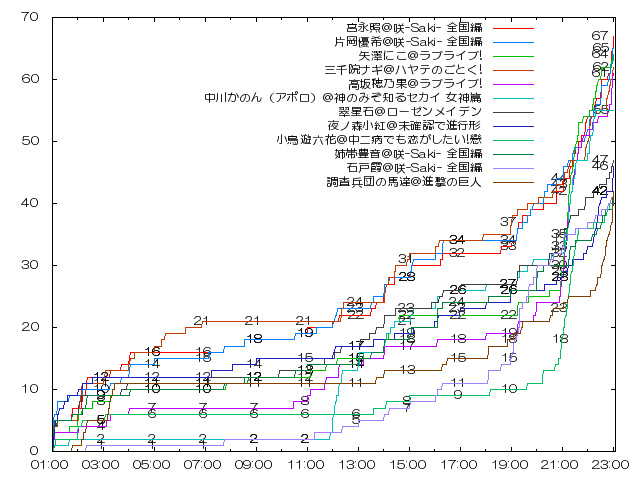
\includegraphics[width=.8\textwidth]{images/graph0916.jpg}

0916是打捞的日子,本战一回战阵亡的角色还有复活的机会。

两个\uline{钉宫}开场和中场一直表现很好,领先全场。为了给\uline{钉宫}的机会,\uwave{麻将}也一直在控票保持\uline{卷饼}和\uline{大小姐}的首位——值得一提的是,似乎还有本土\uline{钉}厨也在做相同的事。\uline{钉宫}的首位优势全天都在保持着。

中午小爆了几票\uline{中川花音}形成了直线,这一小段直线被称为「加农炮(Cannon炮)」,而由于\uline{花音}没有怎么连\uline{艾露西}和\uline{千寻}(实际上是因为程序不够智能不会控制连记),\uline{东山}党的呼声终于被带出来了,\uline{自由}的目的之一达成。

\uwave{麻将}还是一如既往地捞人,除了7个败退的,还有一匹\uline{马}。海底开始,本土照厨开始刷\uline{照姐}——当时也\uline{麻将}依然不知道本土厨\uline{照}。同时海外的\uwave{LL}也开始爆票,大量「\uline{妮可}-\uline{果果}-\uline{六花}-\uline{麻耶}」的连记开始在票楼横行——大混战还敢明目张胆地这么连记总是有点不妥的。顺便提及一下,中期的偶像连记,包括\uwave{爱马仕}、\uwave{LL}、\uline{花音},也是作为一个梗带起来的。

复活赛的赛制是一票最多四个人,而这么多角色必然产生分票,所以可以看到很多个位数的票,其中不乏一些非常有名的角色。而且在比赛后期会演变成少数几个人争夺晋级机会的角逐,票少的会更少,票多的会更多,造成了严重两极分化。复活的难度在一回战就表现了出来,这一仗下来,应该意识到捞人的难度,尤其是三回战只能捞8个的情况下,各阵营不应该把角色轻易放进复活。

复活赛实在是过于混乱了,没有厨的支持根本不可能晋级,就连晋级的\uwave{人偶}也是大厨怀念旧时代进行的打捞。一回战还有散票支持的身影,但是二回战三回战的时候就只有多重屋的肆虐了。在多重屋的票力面前,赛制也是空谈;在运营的砍票面前,票力也是空谈。

\chapter{本战二回战}

二回战是今年日萌的过渡期,是以三连记为基础的海外阵营稳定共赢阶段,以\uwave{麻将}为主导的海外四家产生了频繁的合作,而\uwave{麻将}与\uwave{LL}矛盾也是这个时期酝酿的。

\section{09/19(金) A2-1 C2-2 E2-1}

\VoteTable{
 投票数:624レス 発行コード数:795\\
 A2-1組\\
 1位 393票 高鴨穏乃@\Saki\\
 2位 194票 南夏奈@みなみけ 夏やすみ\\
 C2-2組\\
 1位 371票 鹿目まどか@\Madomagi\\
 2位 247票 園城寺怜@\Saki\\
 E2-1組\\
 1位 335票 東條希@ラブライブ!\\
 2位 257票 福路美穂子@\Saki
}

0919 为了避免\uline{稳乃}重演12年被\uline{久}厨克死的命运,\uwave{麻将}决策让出\uline{托奇}和\uline{福妈},以换取\uline{稳乃}的平稳晋级。这不仅是为了\uwave{麻将}的利益,同时也是为了各阵营之间的平衡,保送\uline{鹿目圆}和\uline{东条希}。所以所谓的萌王对战变得没什么悬念——复活赛制的存在让动刀子变得意义不大,这也是\textbf{第四次\uwave{圆}\uwave{麻}合作}。

可以注意到这天票数很多,原因在于海外的决策本土并不知情,整个白天本土\uwave{麻将}都在努力对抗海外三连记,海外\uwave{麻将}心里总是过意不去的,但是也只能听之任之了。为了给本土一个安慰,决定饭后开始放票,为了防止产生不必要的误会,提前向\uwave{圆脸}和\uwave{LL}告知了饭后的放票。这天的海底也是出了不少,煮了不少。这场之后,本土开始怨恨\uwave{圆脸}\uline{UMB}连记,骂\uline{鸭子}为「猿(猴子)」,本来就不人气的\uline{鸭子}越发成为了卖队友的罪人,风评被害。

暂不表本土。

赛后,\uline{兰博}找到\uline{自由}提到了一个事实,就是整个全天的三连记大部分都是\uwave{圆脸}一家出的,而\uwave{LL}则是以逸待劳,没有出太多票,并且没有向\uwave{圆脸}表达谢意。\uline{自由}随之去尝试了一下\uwave{LL}的态度,提出了「二回战两送(\uline{希}、\uline{姬})一还(\uline{凛}),三回战一送(\uline{希})一还(\uline{海})」的交换,\uline{梨落}表示不同意并且开始骂人,态度恶劣。\uline{自由}不再接话,回去便开了个新讨论组叫做『LLanti』,表面上的\uwave{麻}\uwave{拉}关系在\uline{流子}的维系之下仍然存在,但自此内部与\uwave{LL}不再两立,反\uwave{LL}计划讨论出炉——二回战A死\uline{海爷},三回战送走\uline{小鸟}。这是\textbf{第三次\uwave{麻}\uwave{拉}矛盾},也是反\uwave{LL}剧本写成之时。\uwave{麻将}开始暗中蓄力,以求一击必胜之日。

是日,基于手动VG连线的~\verb=c4vg.php=开始派上用场,\uwave{麻将}的领票效率得到了进一步提升。

\section{09/20(土) A2-2 C2-1 E2-2}

\VoteTable{
 投票数:332レス 発行コード数:394\\
 A2-2組\\
 1位 191票 食蜂操祈@\Railgan\\
 2位 133票 メグ(奈津恵)@ご注文はうさぎですか?\\
 C1-1組\\
 1位 180票 越谷夏海@のんのんびより\\
 2位 126票 竜宮レナ@ひぐらしのなく頃に拡 -アウトブレイク-\\
 E1-2組\\
 1位 176票 愛宕絹恵@\Saki\\
 2位 134票 高尾部長@ディーふらぐ!
}

0920 是平稳的第四次\uwave{电}\uwave{麻}合作,\uwave{麻将}和\uwave{电磁炮}的关系不管是有言还是无言,都是大阵营之间友好的默契。\uwave{麻}\uwave{拉}的矛盾再怎么也影响不到\uwave{麻将}与其他阵营的关系。

\uline{食蜂}顺利晋级,并且\uwave{麻将}考虑到\uwave{电磁}作为有责任感的大阵营,不会做出出格的举动,就帮助保送了二回战所有的\uwave{电磁}。

\section{09/21(日) B2-1 D2-2 F2-1}

\VoteTable{
 投票数:329レス 発行コード数:416\\
 B2-1組\\
 1位 204票 アリス·カータレット@きんいろモザイク\\
 2位 100票 ニンフ@そらのおとしものFinal 永遠の私の鳥籠\\
 D2-2組\\
 1位 148票 末原恭子@\Saki\\
 2位 65票 上重漫@\Saki\\
 F2-1組\\
 1位 197票 美樹さやか@\Madomagi\\
 2位 128票 大宮忍@きんいろモザイク
}

0921 是\uline{恭子}与\uline{小漫}的相爱相杀——这也是\uwave{麻将}预定好的剧情杀,剧本就是这么写成并演出的,孰攻孰受也是清晰明了。

二预的\uline{妮姆芙}由于双杀\uwave{麻将}的使命已经达成,就没什么票了。\uwave{圆脸}也是足够仁义,虽然\uline{蓝毛}胜了\uline{忍叔},但是另一边\uline{爱丽丝}顺利晋级。所谓对新番的送一换一,便是如此。这也是海外阵营对新番的共同态度,在不侵犯阵营利益的前提下尽可能保送可爱新番。

\section{09/22(月) B2-2 D2-1 F2-2}

\VoteTable{
 投票数:499レス 発行コード数:569\\
 B2-2組\\
 1位 253票 絢瀬絵里@ラブライブ!\\
 2位 237票 丹生谷森夏@中二病でも恋がしたい!戀\\
 D2-1組\\
 1位 307票 由比ヶ浜結衣@やはり俺の青春ラブコメはまちがっている。\\
 2位 143票 カズミ=シュリーレンツァウアー@極黒のブリュンヒルデ\\
 F2-2組\\
 1位 302票 千石撫子@〈物語〉シリーズ~セカンドシーズン\\
 2位 139票 大宮勇@きんいろモザイク
}

0922 是\uwave{LL}所谓的大战,因为对手是\uline{运营森}。至于\uline{运营森}是怎么来的呢,是在于去年的code发行所留下的Cookies里面有「morisama」的字样——code屋其实是\uline{森}蜜?由于很多人搞不清楚\uline{运营}和\uline{code屋}的区别,所以就叫成\uline{运营森}了。不过今年不一样,新code屋\uline{OAa}在实行了(84)规制案之后,眼看还是管不住多重屋,就撒手跑路了,所以也不存在运营亲女儿是\uline{森夏}一说。

京都衰落的日萌,\uline{森夏}毫无战斗力,当然之前\uwave{麻将}并不知道这一点。军师主张这场用\uline{森夏}再试一试\uwave{LL}的实力,这一试却试出来\uline{森夏}的战五属性了。\uwave{麻将}了解到了\uwave{LL}的实力不过250,战五渣的\uline{森夏}输得也是理所当然。

至于隔壁\uline{团子}和\uline{抚子}的保送,实际上也是看散票的偏向的吧。

\section{09/23(祝) G2-2 I2-1 K2-2}

\VoteTable{
 投票数:434レス 発行コード数:546\\
 G2-2組\\
 1位 230票 初春飾利@\Railgan\\
 2位 188票 ココア(保登心愛)@ご注文はうさぎですか?\\
 I2-1組\\
 1位 233票 鹿倉胡桃@\Saki\\
 2位 165票 ジブリール@ノーゲーム·ノーライフ\\
 K2-2組\\
 1位 224票 チノ(香風智乃)@ご注文はうさぎですか?\\
 2位 181票 藤宮香織@一週間フレンズ。
}

0923 是第五次\uwave{电}\uwave{麻}合作,\uline{初春}和\uline{胡桃}轻松晋级。考虑到\uwave{点兔}连记,\uwave{麻将}曾经讨论过是不是要出手\uline{心爱},这样三回战就不再是一\uwave{麻}对三\uwave{炮}的不利局势了。为了保持与\uwave{电磁}的友好关系,就保送了\uline{初春}到三回战。

\uline{胡桃}接连晋级,其中\uline{自由}作为\uline{丰田萌绘}的古参厨也是幕后推手。不过\uline{胡桃}连续两次以233票晋级,这个真的不是故意的,纯属偶然和巧合,只能说是上天眷顾吧。

\section{09/24(水) G2-1 I2-2 K2-1}

\VoteTable{
 投票数:355レス 発行コード数:529\\
 G2-1組\\
 1位 192票 フレンダ=セイヴェルン@\Railgan\\
 2位 118票 名瀬美月@境界の彼方\\
 I2-2組\\
 1位 188票 桐崎千棘@ニセコイ\\
 2位 137票 千夜(宇治松千夜)@ご注文はうさぎですか?\\
 K2-1組\\
 1位 219票 佐倉杏子@\Madomagi\\
 2位 124票 東横桃子@\Saki\\
 K2-1組 (面票)\\
 2位 99票 東横桃子@\Saki\\
}

0924 应该是不知道第几次\uwave{圆炮}合作了,\uline{自由}向两家交待了一下带上\uline{东山}的\uline{千棘},然后就默默去给\uline{桃子}刷隐票了。最后\uline{桃子}面票99,隐票接近30。不得不说刷隐票比较麻烦,效率不高,需要花心思去做。

这一场也是\uwave{圆}\uwave{麻}本战最后一回冲突,\uwave{圆脸}约定,此战保送\uline{杏子}之后,便全心与\uwave{麻将}达成联盟关系。

\section{09/26(金) H2-2 J2-1 L2-2}

\VoteTable{
 投票数:496レス 発行コード数:785\\
 H2-2組\\
 1位 283票 御坂妹(ミサカ10032号)@\Railgan\\
 2位 178票 戦場ヶ原ひたぎ@〈物語〉シリーズ~セカンドシーズン\\
 J2-1組\\
 1位 295票 愛宕洋榎@\Saki\\
 2位 152票 水銀燈@ローゼンメイデン\\
 L2-2組\\
 1位 314票 暁美ほむら@\Madomagi\\
 2位 87票 姫柊雪菜@ストライク·ザ·ブラッド\\
 3位 77票 猪熊陽子@きんいろモザイク
}

0926 又迎来了海外三连记,作为\textbf{第七次\uwave{圆}\uwave{麻}合作}和\textbf{第六次\uwave{电}\uwave{麻}合作},\uline{御坂妹}、\uline{爱宕姐}、\uline{晓美焰}都得到了保送。尤其是由于一回战\uline{阳子}和\uline{雪菜}平票,这下直接分票,\uline{晓美焰}轻松晋级,连给人A的机会都没有,想趁机A死\uwave{圆脸}的倒也死心了。

\uline{爱宕姐}打\uline{水银灯},实在是一件心塞的事。\uline{汞}不八,\uline{焰}不八,同场竞技,可惜因为\uwave{麻将}三回战\uline{爱姐}婊\uline{受久}的剧本,\uline{汞}不八的传说只能继续了。所谓命运无非如此——没有厨子的支持,怨念再深也没什么用。因为简体字的关系,「水银灯」在票楼里显示成了「{\mincho 水$\!\!$□$\!\!$灯}」,不知道是哪位海外大厨的支援。虽然很惋惜\uline{水口灯},也只能惋惜而无能为力了。

\section{09/27(土) H2-1 J2-2 L2-1}

\VoteTable{
 投票数:229レス 発行コード数:371\\
 H2-1組\\
 1位 131票 神代小蒔@\Saki\\
 2位 69票 鶴田姫子@\Saki\\
 J2-2組\\
 1位 157票 竹井久@\Saki\\
 2位 71票 木下林檎(草壁ゆか)@のうりん\\
 L2-1組\\
 1位 125票 園田優@桜Trick\\
 2位 82票 船堀@ディーふらぐ!
}

剧本就是剧本,0927 保送\uline{久帝}中坚战。\uline{公主}和\uline{姬子}的取舍,首推\uwave{全国篇}的新人。

另一边也能保送\uwave{樱T}独苗\uline{园田优}进入三回战。这大概没什么可说的。

\section{09/28(日) M2-1 O2-2 Q2-1}

\VoteTable{
 投票数:419レス 発行コード数:589\\
 M2-1組\\
 1位 265票 松実玄@\Saki\\
 2位 139票 三峰真白@未確認で進行形\\
 O2-2組\\
 1位 265票 新子憧@\Saki\\
 2位 147票 小路綾@きんいろモザイク\\
 Q2-1組\\
 1位 314票 原村和@\Saki\\
 2位 83票 星空凛@ラブライブ!
}

这个时期的\uwave{麻将},从维持曲线的出票到饭后到海底,都已经驾轻就熟了。0928 \uwave{麻将}三连——\uline{玄憧和}这三员大将,哪个都不能弃的地位。\uline{小路绫}可以说赛前一直在有人吹,不过遇到了\uline{新子憧},作为\uwave{麻将}厨+\uline{东山}厨的\uline{自由},即使是再不舍,也必须保送。同时因为与\uwave{LL}达成了暗里的敌对关系,也决定下一场A死最大对手\uline{园田海未}。\uwave{麻将}的三连记有条而不紊地进行着,实际上已经暗流涌动,酝酿着\uwave{麻将}的阴谋。

日前,\uline{梨落}来找\uline{自由}要下一场的连记,为了拖延\uwave{LL}准备日租服务器,\uline{自由}没有立刻回复,而是拖到了中午通知了他下一场隔空对轰。实际上日租服务器确实不好租,尤其是日文服务器基本上没货,这一点成功拖延了\uwave{LL}的票力。而「\uwave{麻}厨的服务器上连日语输入法都没有」这一事实,则对\uwave{麻将}有着强大的优势——\uwave{麻将}的服务器随拿随用,部署好PHP就可以自动化了,而且不拘谨于服务器操作系统和语言。实际上\uwave{麻将}早有了Linux的服务器,没有图形界面对\uwave{麻将}反而是优势。

\section{09/29(月) M2-2 O2-1 Q2-2}

\VoteTable{
 投票数:826レス 発行コード数:1001\\
 M2-2組\\
 1位 501票 蒼星石@ローゼンメイデン\\
 2位 276票 宇迦之御魂神(うか様)@いなり、こんこん、恋いろは。\\
 O2-1組\\
 1位 476票 雪ノ下雪乃@やはり俺の青春ラブコメはまちがっている。\\
 2位 337票 園田海未@ラブライブ!\\
 Q2-2組\\
 1位 487票 天江衣@\Saki\\
 2位 325票 五河琴里@デート·ア·ライブII
}

0929 各种信任的破裂。为了防止\uwave{电磁}\uwave{LL}达成联盟破坏\uwave{麻将}的剧本,\uwave{麻将}找来了\uwave{圆脸}帮忙,并且在表面上没有提到这一点。开场引领了「\uline{小衣}-\uline{雪乃}」的连记,就和\uwave{LL}正式刚上了。在\uwave{麻将}强大的票力压制下,一个夜里就拉开80+。随着\uwave{LL}厨的起床,比赛开始进入白热化。\uwave{麻将}一边与\uwave{LL}保持着相当的票差,一边向\uwave{圆脸}哭穷表示没票。作为\textbf{第八次\uwave{圆}\uwave{麻}合作},\uwave{麻将}获得了\uwave{圆脸}100+票的支援,而本身票力就已经很强大的\uwave{麻将},通过这些票爆出了惊天的海底,还煮了100+。最终\uwave{LL}败下阵来,\uline{天江衣}连记\uline{雪乃}获胜,\uline{苍星石}也突破了500票,发行也破了1000,是为今年日萌第一场千票战。\uwave{LL}的极限票力表现为海未的337,也让\uwave{麻将}对围剿\uwave{LL}信心十足。

赛后毫无疑问产生了\textbf{第四次\uwave{麻}\uwave{拉}矛盾},\uline{梨落}扬言下一轮A回来300票让\uwave{麻将}吃不了兜着走。\uline{自由}也与\uline{ako}蜜的\uline{羽毛}产生了不小的矛盾,因为\uline{自由}骂道「我看不起A自己本命的厨子」,也导致后来\uline{羽毛}处处点着\uline{自由}的名字骂。实际上\uline{自由}也是A死了本命的\uline{海爷},说出这种话也毫无道理。

\section{09/30(火) N2-1 P2-2 R2-1}

\VoteTable{
 投票数:184レス 発行コード数:306\\
 N2-1組\\
 1位 87票 比企谷小町@やはり俺の青春ラブコメはまちがっている。\\
 2位 67票 綾瀬千早@ちはやふる わがみよにふるながめせしまに\\
 P2-2組\\
 1位 79票 遠坂凛@Fate/kaleid liner プリズマ☆イリヤ\\
 2位 74票 古手梨花@ひぐらしのなく頃に拡 -アウトブレイク-\\
 R2-1組\\
 1位 142票 九条カレン@きんいろモザイク\\
 2位 37票 藍羽浅葱@ストライク·ザ·ブラッド
}

0930 是大战之后的休息,可怜不用说都被本土保送了,\uline{自由}这\uline{东山}厨也是当得轻松。\uline{凛}和\uline{梨花}都是老将,孰赢孰败作为悬念也一直持续到了比赛结束。\uwave{春物}的\uline{小町}对上乙女番的\uwave{花牌},胜出也是可以预料到的。

\section{10/01(水) N2-2 P2-1 R2-2}

\VoteTable{
 投票数:373レス 発行コード数:470\\
 N2-2組\\
 1位 226票 辻垣内智葉@\Saki\\
 2位 110票 東兎角@悪魔のリドル\\
 P2-1組\\
 1位 229票 シャロ(桐間紗路)@ご注文はうさぎですか?\\
 2位 125票 黒猫(五更瑠璃)@俺の妹がこんなに可愛いわけがない。\\
 R2-2組\\
 1位 195票 南ことり@ラブライブ!\\
 2位 145票 橘万里花@ニセコイ
}

骂战归骂战,\uwave{麻将}还是不想直接和\uwave{LL}撕破脸。1001 国庆大家都去现充了,也就没把\uline{小鸟}在二回战摁死,而是举行了\textbf{\uwave{麻}\uwave{拉}短暂合作之一}。\uwave{智叶}作为\uwave{麻将},轻松保送。二线的\uline{纱路}成了\uwave{点兔}独苗,也被保送了,\uline{黑猫}无厨自然不行。\uline{小鸟}也顺利通过,毕竟没有什么\uwave{伪恋}阵营和\uline{阿澄}阵营。

是日,在\uline{末原}的提议下,『LLanti』讨论组更名『咲豚总圈』,标志着\uline{末原}的权力得到肯定。

\section{10/03(金) S2-2 U2-1 W2-2}

\VoteTable{
 投票数:251レス 発行コード数:292\\
 S2-2組\\
 1位 130票 小泉花陽@ラブライブ!\\
 2位 113票 一条蛍@のんのんびより\\
 U2-1組\\
 1位 173票 白井黒子@\Railgan\\
 2位 65票 八九寺真宵@〈物語〉シリーズ~セカンドシーズン\\
 W2-2組\\
 1位 110票 橘佳奈@極黒のブリュンヒルデ\\
 2位 103票 土御門夏目@東京レイヴンズ
}

1003 是\uwave{电磁}和\uwave{LL}携手晋级,还是那句话,在大阵营的联携之下,任何新番都是渣渣。

\section{10/04(土) S2-1 U2-2 W2-1}

\VoteTable{
 投票数:403レス 発行コード数:633\\
 S2-1組\\
 1位 255票 清水谷竜華@\Saki\\
 2位 102票 五月七日くみん@中二病でも恋がしたい!戀\\
 U2-2組\\
 1位 203票 大星淡@\Saki\\
 2位 142票 薄墨初美@\Saki\\
 W2-1組\\
 1位 229票 西木野真姫@ラブライブ!\\
 2位 166票 夢乃マホ@\Saki
}

1004 按照之前的约定,\uwave{麻将}弃掉了\uline{真帆}而送给了\uline{真姬},这是\textbf{\uwave{麻}\uwave{拉}短暂合作之二}。

\uline{自由}曾经提出过一个等价关系,\uline{和}对\uline{凛}=\uline{真姬}对\uline{真帆},所以该让就得让。不过由于\uline{真姬}一回战的直线爆票逆转导致的风评被害,\uline{真姬}吃到了不少来自本土的A票,虽然在海外强大的票力之下这些A票毫无作用,不过也能看出来\uwave{LL}的声誉已经在本土变得很黑了。

这场海外\uwave{麻将}没怎么出票,而是把这天的出票交给了\uwave{LL}——老老实实连\uline{龙华}谁都没坏处,\uline{笨淡}还是\uline{四喜}是你们自己的问题。关于\uline{笨淡}和\uline{小四喜}的取舍,当时是想保送\uline{小四喜}到三回战,然后把送\uline{黑子}一个32强的。\uline{流子}表示想要厨\uline{笨淡},也就变成了保送\uline{笨淡}32强的剧本。有时候弃保就是这么随意吧。

\section{10/05(日) T2-2 V2-1 X2-2}

\VoteTable{
 投票数:546レス 発行コード数:718\\
 T2-2組\\
 1位 387票 御坂美琴@\Railgan\\
 2位 139票 越谷小鞠@のんのんびより\\
 V2-1組\\
 1位 338票 松実宥@\Saki\\
 2位 106票 小木曽雪菜@WHITE ALBUM2\\
 X2-2組\\
 1位 391票 宮永咲@\Saki\\
 2位 105票 四糸乃@デート·ア·ライブII
}

1005 是\textbf{第七次\uwave{电}\uwave{麻}合作},这里是两家主角的\uline{美琴}和\uline{saki}同时登场,获得了两家极大的重视,表示要轰出来高票。两家的连记也不是太死的,当时确实是\uwave{电磁}考虑到「不想再被打成多重阵营」,从萌文到连记都是处处小心。\uline{宥姐}、\uline{炮姐}、\uline{魔王}的票差阶梯,代表着\uline{自由}对这三个角色的重视程度。带着这个私心,把\uline{咲}的票数控到了略微超过\uline{炮姐}的程度,而\uline{宥姐}则被远远拉开。而且最后把票控到了400以内,也是考虑到不要过于招摇——\uwave{电}\uwave{麻}要是动真格的哪家轰不出来400啊。

\section{10/06(月) T2-1 V2-2 X2-1}

\VoteTable{
 投票数:398レス 発行コード数:574\\
 T2-1組\\
 1位 197票 結城明日奈(アスナ)@ソードアート·オンライン Extra Edition\\
 2位 155票 リゼ(天々座理世)@ご注文はうさぎですか?\\
 V2-2組\\
 1位 260票 巴マミ@\Madomagi\\
 2位 100票 夜刀神十香@デート·ア·ライブII\\
 X2-1組\\
 1位 254票 佐天涙子@\Railgan\\
 2位 86票 鷺森灼@\Saki
}

1006 没想到的是\uline{亚丝娜}被\uwave{电磁}保送了,\uwave{炮}\uwave{娜}一家这事,\uwave{麻将}也是这场才知道。即便是考虑到三回战\uline{泪爷}对\uline{魔王}会产生相当大的威胁,但还是基于阵营之间的信任,所以二回战没有A\uwave{电磁}。

\section{10/08(水) 敗者復活2回戦}

\VoteTable{
 投票数:564レス 発行コード数:751\\
 1位 81票 園田海未@ラブライブ!\\
 2位 77票 調査兵団の馬達@進撃の巨人\\
 3位 76票 星空凛@ラブライブ!\\
 4位 75票 宮永照@\Saki\\
 5位 74票 高坂穂乃果@ラブライブ!\\
 6位 73票 矢澤にこ@ラブライブ!\\
 7位 72票 丹生谷森夏@中二病でも恋がしたい!戀\\
 8位 71票 三千院ナギ@ハヤテのごとく!\\
 8位 71票 中川かのん(アポロ)@\Kaminomi\\
 10位 69票 五河琴里@デート·ア·ライブII\\
 11位 67票 ココア(保登心愛)@ご注文はうさぎですか?\\
 12位 66票 園城寺怜@\Saki\\
 13位 65票 片岡優希@\Saki\\
 14位 62票 小瀬川白望@\Saki\\
 14位 62票 リゼ(天々座理世)@ご注文はうさぎですか?\\
 16位 61票 姉帯豊音@\Saki\\
 16位 61票 福路美穂子@\Saki\\
 ━━━━━━━ここまで敗者復活2回戦進出━━━━━━━\\\zihao{6}
 18位 60票 翠星石@ローゼンメイデン\\
 19位 55票 ゆの@ひだまりスケッチ~沙英·ヒロ~卒業編\\
 20位 47票 夜ノ森小紅@未確認で進行形\\
 21位 45票 司波深雪@魔法科高校の劣等生\\
 22位 42票 小野寺小咲@ニセコイ\\
 22位 42票 藤宮香織@一週間フレンズ。\\
 24位 38票 越谷小鞠@のんのんびより\\
 25位 37票 小路綾@きんいろモザイク\\
 26位 36票 大宮忍@きんいろモザイク\\
 27位 33票 千夜(宇治松千夜)@ご注文はうさぎですか?\\
 28位 32票 小鳥遊六花@中二病でも恋がしたい!戀\\
 28位 32票 薄墨初美@\Saki\\
 30位 31票 一条蛍@のんのんびより\\
 31位 29票 石戸霞@\Saki\\
 32位 28票 東横桃子@\Saki\\
 32位 28票 黒猫(五更瑠璃)@俺の妹がこんなに可愛いわけがない。\\
 32位 28票 夢乃マホ@\Saki\\
 35位 25票 四糸乃@デート·ア·ライブII\\
 36位 24票 水銀燈@ローゼンメイデン\\
 37位 23票 上重漫@\Saki\\
 38位 20票 白@ノーゲーム·ノーライフ\\
 39位 17票 瑞原はやり@\Saki\\
 39位 17票 龍門渕透華@\Saki\\
 39位 17票 鶴田姫子@\Saki\\
 42位 14票 姫柊雪菜@ストライク·ザ·ブラッド\\
 43位 13票 黒羽寧子@極黒のブリュンヒルデ\\
 43位 13票 夜刀神十香@デート·ア·ライブII\\
 45位 11票 宮内れんげ@のんのんびより\\
 45位 11票 真紅@ローゼンメイデン\\
 45位 11票 三峰真白@未確認で進行形\\
 45位 11票 鷺森灼@\Saki\\
 49位 9票 湊智花@ロウきゅーぶ!SS\\
 49位 9票 戦場ヶ原ひたぎ@〈物語〉シリーズ~セカンドシーズン\\
 51位 8票 カズミ=シュリーレンツァウアー@極黒のブリュンヒルデ\\
 51位 8票 小木曽雪菜@WHITE ALBUM2\\
 53位 7票 ニンフ@そらのおとしものFinal 永遠の私の鳥籠\\
 53位 7票 高尾部長@ディーふらぐ!\\
 53位 7票 名瀬美月@境界の彼方\\
 56位 6票 橘万里花@ニセコイ\\
 57位 5票 宇迦之御魂神(うか様)@いなり、こんこん、恋いろは。\\
 57位 5票 古手梨花@ひぐらしのなく頃に拡 -アウトブレイク-\\
 59位 4票 ステファニー·ドーラ(ステフ)@ノーゲーム·ノーライフ\\
 59位 4票 メグ(奈津恵)@ご注文はうさぎですか?\\
 59位 4票 ジブリール@ノーゲーム·ノーライフ\\
 59位 4票 五月七日くみん@中二病でも恋がしたい!戀\\
 63位 3票 竜宮レナ@ひぐらしのなく頃に拡 -アウトブレイク-\\
 63位 3票 船堀@ディーふらぐ!\\
 63位 3票 土御門夏目@東京レイヴンズ\\
 66位 2票 南夏奈@みなみけ 夏やすみ\\
 66位 2票 大宮勇@きんいろモザイク\\
 66位 2票 木下林檎(草壁ゆか)@のうりん\\
 66位 2票 猪熊陽子@きんいろモザイク\\
 66位 2票 東兎角@悪魔のリドル\\
 66位 2票 藍羽浅葱@ストライク·ザ·ブラッド\\
 66位 2票 八九寺真宵@〈物語〉シリーズ~セカンドシーズン\\
 73位 1票 綾瀬千早@ちはやふる わがみよにふるながめせしまに
}

1008 是复活二回战,目的有三:捞\uline{马}、捞\uwave{麻}、捞\uline{花音}。由于和\uwave{LL}关系的闹僵,这天\uline{自由}没给\uwave{LL}出多少票,这跟复活一回战时\uline{自由}还把自己当\uwave{LL}厨时积极打捞\uwave{LL}的表现已经发生了很大的变化。\uline{三千}和\uline{卷饼}虽然没了「\uline{钉宫}百胜」,但是也有着本土的支持坚持到了晋级。\uline{琴里}是世萌萌王,为了照应这个捏他,\uwave{麻将}和\uwave{圆脸}也在打捞\uline{琴里}。不过\uwave{圆}\uwave{麻}没怎么管\uline{森夏},反倒是\uwave{电}\uwave{L}对打捞\uline{森夏}很在意的样子,依然在饭后爆了大量的四连记捞上来了\uline{森夏}——大概是因为\uwave{LL}厨是当年京厨的缘故?

打捞\uline{花音}是\uline{东山}厨一生的追求(拍飞),即使是歌词爆票有何不可。只有\uwave{麻将}的打捞,老将\uline{托奇}、\uline{福妈}和新人\uline{小白}、\uline{丰音}成为了保送对象。本土厨\uline{照},所以\uline{照姐}刷了\uwave{麻将}的最高票。

不过这场最有意思的是\uline{马达}居然是第二位啊!其实说说\uline{马达}的故事,还是津津乐道的。这天晚上简直咲cry,海底时间运营把「咲」这个字给设置成NGword了,所有包含「咲」这个字的投票都投不出去——一部分票自动出到了备用板,但是更多的还是包含着\uline{马达}却没有\uwave{麻将}的票出到了主票楼——这直接导致了\uline{马达}的票数比\uwave{麻将}还多。本土也开始狂欢了,你不让我投\uwave{麻将},那我就投\uline{马儿}啊,也开始跟风刷\uline{马}了,而且人比机器刷得更起劲。

结果这次的最大输家不是\uwave{麻将},而是\uline{小野寺小咲}——直接被NG得SGG了,\uline{RUN}也是搬起石头砸自己的脚。最大的赢家也不是刷到了首位的\uwave{LL},而是本土对\uline{马达}的狂欢,\uline{RUN}的不正行为被打脸好不痛快。
\\

是日,由\uline{兰博}提议,\uwave{圆}\uwave{麻}正式成立了神圣联盟『Holy League』,双方表示合作到底。
\\[1em]

二回战期间也是\uwave{麻将}科技稳定发展的阶段。服务器的黑魔法因为\uwave{麻将}的滥用,被卖家警告以后废弃了。半自动的抓票辅助程序得以熟练运用。全自动的挖掘机也是二回战开发出来的。票面生成器进一步得到改进,票面的自动填充和投放也使得投票不再限于code。海底多机联合爆票技术也成功运用起来。UA列表也得以极大丰富。可以说二回战的\uwave{麻将}已经成为了至少是近几年日萌科技水平最高的阵营。所谓「程序员萌」不过如此,去年是「我\uwave{圆}科技天下第一」,今年倒也该吹吹「我\uwave{麻}科技天下第一」了吧233。

\chapter{本战三回战}

三回战决出的是24强,结合复活战决出8个,一共32人进入季后赛。这也就是组决赛,决定着八强的分羹,也是各大阵营非常重视的阶段。虽然由于赛制的改变,三回战不再表现得像之前那么重要,但是这次的三回战却因为砍票,\uwave{麻将}与\uwave{LL}产生了最大的撕逼之战,打破了之前还相对和谐的海外关系,比赛陷入混乱。砍票也彻底断送了\uwave{LL}和\uwave{电磁}之后的前途,四大阵营一轮之内也变成了\uwave{圆}\uwave{麻}萌。

\section{10/11(土) A3 G3}

1011 可以说是2014日萌的「关原合战」,此役拿下,三回战格局已定。

\VoteTable{
 投票数:1139レス 発行コード数:1328\\
 A3組\\
 1位 635票 高鴨穏乃@\Saki\\
 2位 502票 食蜂操祈@\Railgan\\
 G3組\\
 1位 589票 初春飾利@\Railgan\\
 2位 335票 フレンダ=セイヴェルン@\Railgan
}

\Graph{1011a}

这场\uwave{电磁}选择了对抗\uwave{麻将}的道路,毕竟作为三\uwave{电磁}出场,阵营肯定会偏向自家人的连记。为了保证胜算,\uwave{电磁}和\uwave{LL}达成了合作,据说当天两家合计使用了40+台的服务器。对此一无所知的\uwave{麻将},赛前一天从\uwave{圆脸}得知了\uwave{电}\uwave{L}联合的事情。为了不把比赛演变成四家合战,尽量推迟决战,\uline{自由}向\uwave{电}\uwave{L}提议还是让这场称为\uwave{电磁}和\uwave{麻将}单挑,并且放言「若\uwave{LL}出票,则\uwave{圆脸}也出手」。一时虽表面达成了妥协,但实际上四家暗中都开始了准备。比赛虽说是\uwave{电磁}对\uwave{麻将},但是\uwave{LL}和\uwave{圆脸}也耐不住寂寞还是参与了进来,那么今年\uwave{圆}\uwave{麻}对\uwave{电}\uwave{L}的四家超多重合战也正式开始。

赛前运营\uline{RUN}突然做出了奇怪的举动,在投票须知中加了一行字「{\mincho ※他者のコピペ投票、無関係の台詞のみを萌え文に使用するなどの行為はおやめください。場合によっては運営の判断で無効とする可能性があります。}\footnote{请不要复制粘贴别人的投票、把没有关系的台词作为萌文使用。运营有可能视情况将这些票视为无效票。}」这意味着运营有可能根据萌文采取意识流砍票。而之前一直使用台词萌文的\uwave{麻将}立刻意识到了问题的严重,开始紧急编写萌文。另一方面,本土\uwave{麻将}也注意到了这点,在票楼贴出了\uline{高鸭稳乃}的一系列性格特点,成为了海外\uwave{麻将}萌文的重要参考,也提示了\uwave{麻将}后期萌文的来源。

\uwave{电磁}强大的半夜爆票能力依然让人叹为观止,开场一片混乱之后,\uwave{电磁}首先确立了领先地位,两家半夜都在维持曲线,但显然\uwave{麻将}的斜率不如\uwave{电磁},到了白天被拉开70票。这个票差一直延续了下去,\uwave{麻将}尝试了几次小型爆票来试探是否\uwave{电磁}在控票。终于到了黄昏时刻,\uwave{麻将}发现\uwave{电磁}已经开始用上个小时的票额来填充票差了,这正是反击之时。由于明显是\uwave{LL}票尾的票出现,\uwave{麻将}也放心大胆地接来了\uwave{圆脸}支援的200票,随着白天囤积的票开始了爆票。\uwave{麻将}强劲的海底爆票一旦开始,便无人可挡,两个小时,\uwave{麻将}完成了追平,开始了反超之旅。最后一个小时更是惊天海啸,深山之主\uline{高鸭稳乃}在票楼正式宣布——这里已经不是你的领域了。山深雾厚,超能力被封印,\uline{猴子}翻过了三座\uwave{电磁}大山,拿下来32强名额。

\uwave{麻将}最后依然煮了近200票,并且几乎全程保持了票数占发行量的「半数优势」,可谓是绝对的票力领先,而所使用服务器不过5台。至于\uwave{电磁}为何40台服务器还这样票力,\uwave{电磁}的总结中提到了后期有些票尾的待发。虽然\uwave{圆}\uwave{麻}并未正式互相交流过,但是两家应该都有相似的解待发的技术。

这是唯一一场海外四家都展示了实力的合战,也正式成为2014日萌的分水岭,宣示着\uwave{圆}\uwave{麻}联盟对\uwave{电}\uwave{L}联合的优势,也是\uwave{圆}\uwave{麻}与\uwave{电}\uwave{L}对立的正式体现。\uwave{圆}\uwave{麻}正式发展成为了新一代的「神圣联盟」。

\section{10/12(日) B3 H3}

1012 则是2014年日萌砍票的开始。这几场的砍票情况让人有点措手不及,砍票前的结果是根据票楼情况和当天直播楼报票计算出来的,所以会有不准确的地方,但是为了让大家了解砍票的情况,贴出来有一个感性的认识比较好。

\VoteTables{
 投票数:約468レス\\
 B3組\\
 1位 236票 絢瀬絵里\\
 2位 206票 アリス\\
 H3組\\
 1位 238票 神代小蒔\\
 2位 191票 御坂妹
}{
 投票数:315レス 発行コード数:818\\
 B3組\\
 1位 192票 アリス·カータレット@きんいろモザイク\\
 2位 114票 絢瀬絵里@ラブライブ!\\
 H3組\\
 1位 211票 神代小蒔@\Saki\\
 2位 86票 御坂妹(ミサカ10032号)@\Railgan
}

经过 1011 的大战,\uwave{麻将}和\uwave{电磁}显然都疲惫不堪了。\uline{自由}教\uwave{LL}老实五五开连记,填装好了\uline{爱丽丝}对\uline{绘里}6:5的票面就不管了,反正是自动的。不过事后\uwave{LL}爆料,当时他们并没有五五开连记\uwave{麻将}和\uwave{电磁},而是结成了\uwave{电}\uwave{L}联合,连记大量倾斜\uwave{电磁}的\uline{御坂妹}。按说比安静进行,\uwave{电}\uwave{麻}做着暗部斗争,保送\uline{KKE}晋级就行。不过事情发生了巨变。

运营\uline{RUN}赛前的投票须知把那行字删去了,猜测是因为前日四家日得太特么多了,\uline{RUN}一看妈的砍不完不砍了。后来发现这场票并不多嘛,就开始寻思着砍票了。先前就盯死了\uwave{LL}的\uline{RUN},这回研究了下投票记录,刷刷刷砍了起来。

下午最开始发现票被删了的是\uwave{LL},投出去的票变成了{\mincho <あぼーん>}(a bone),于是开始在直播楼惊呼这一异常情况。了解到这一情况,\uwave{麻将}立刻去调查了,发现\uwave{麻将}的票并没有出现这样的问题。当时\uline{自由}就意识到了是不是\uwave{LL}的投票机制被抓到了把柄,开始提醒\uwave{电}\uwave{L}注意投票手段。\uwave{麻将}的投票虽然是自动的,可一点也不简单,随机大量的UA库、随机的延迟都是值得注意的地方。\uwave{麻将}开始试验如何才能被砍,通过设定特殊的UA和指定特殊的domain成功被运营砍掉,从而了解到此时的\uline{RUN}还是技术砍为主。而\uwave{电}\uwave{L}还是没能抓住要领,一直被砍到了最后比赛结束。\uline{绘里}被活生生砍死,\uline{御坂妹}本来就不够赢的票数则直接砍到了两位数。

这场的砍票是技术砍为主的,早已取得大量技术进步的\uwave{麻将}显然获得了更大的优势。而\uline{爱丽丝}则意外地被砍活,鉴于海外\uwave{麻将}并没有大量连记\uline{爱丽丝}的事实,只能认为确实是散票发挥了强大作用。事实上,这场的技术砍即使是砍\uwave{电}\uwave{L}也没有完全砍光,\uwave{麻将}的票也非没有殃及,散票也有中招的情况。

\section{10/13(祝) C3 I3}

\VoteTables{
 投票数:約300レス\\
 C3組\\
 1位 201票 鹿目まどか\\
 2位 92票 越谷夏海\\\\
 I3組\\
 1位 165票 桐崎千棘\\
 2位 119票 鹿倉胡桃
}{
 投票数:233レス 発行コード数:512\\
 C3組\\
 1位 147票 鹿目まどか@\Madomagi\\
 2位 76票 越谷夏海@のんのんびより\\
 I3組\\
 1位 134票 桐崎千棘@ニセコイ\\
 2位 82票 鹿倉胡桃@\Saki
}

1013 虽然还可以来一场\uwave{圆}\uwave{麻}合作的,不过作为\uline{东山}厨的\uline{自由}和\uline{兰博}达成了保\uline{千棘}的共识。于是\uline{胡桃}被弃掉,\uline{千棘}作为24强最弱被保送。

这场还是有砍票,但是并没有砍太多。四家都在测试运营的砍票规则,就后面来看,\uwave{电磁}和\uwave{LL}的票一如既往被砍,\uwave{圆脸}的被砍票数比\uwave{麻将}稍多,但后期做了改进。
\newpage
\section{10/14(火) D3 J3}

\VoteTables{
 投票数:約375レス\\
 D3組\\
 1位 199票 末原恭子\\
 2位 172票 由比ヶ浜衣\\\\
 J3組\\
 1位 203票 愛宕洋榎\\
 2位 111票 竹井久\\
}{
 投票数:359レス 発行コード数:462\\
 D3組\\
 1位 194票 末原恭子@\Saki\\
 2位 162票 由比ヶ浜結衣@やはり俺の青春ラブコメはまちがっている。\\
 J3組\\
 1位 195票 愛宕洋榎@\Saki\\
 2位 110票 竹井久@\Saki\\
}

1014 的\uwave{麻将}剧本是期待已久的中坚战——\uline{爱姐}婊\uline{受久}。这也正如\uwave{全国篇}剧情表现得一样。

D组\uline{自由}的意思是保送\uline{团子},\uline{末原}则要求保送\uline{恭子}。作为妥协,同意以减少票差的方式保送\uline{恭子},以及复活打捞\uline{团子}。于是这天挖掘机是一场自导自演的游戏——\uline{团子}的票和\uline{恭子}的票都是\uwave{麻将}出着玩的。最后的砍票也只砍掉了很少一部分,这已经证明了\uwave{麻将}「破解」了运营当时的砍票机制。

\section{10/15(水) E3 K3}

\VoteTables{
 投票数:約420レス\\
 E3組\\
 1位 212票 愛宕絹恵\\
 2位 186票 東條希\\\\
 K3組\\
 1位 258票 佐倉杏子\\
 2位 150票 香風智乃
}{
 投票数:337レス 発行コード数:592\\
 E3組\\
 1位 191票 愛宕絹恵@\Saki\\
 2位 125票 東條希@ラブライブ!\\
 K3組\\
 1位 212票 佐倉杏子@\Madomagi\\
 2位 113票 チノ(香風智乃)@ご注文はうさぎですか?
}

终于来到 1015 这场撕逼大战了。看出场角色都不是什么阵营一线,却演变成了14日萌最严重的海外事件。事件的直接结果是\uline{东条希}的败退和\uwave{LL}阵营的倒塌,内部结果是\uwave{麻将}与\uwave{LL}的正式撕逼,\uline{自由}与\uline{梨落}一行恩怨的结成。

赛前的\uwave{LL}在群里问了下\uwave{麻将}的态度,\uline{自由}说了四个字「放手拼散」。这个「放手拼散」是什么意思呢,就是我不投票,让散票投也能赢\uwave{LL},因为还有砍票。

二回战已经把\uline{福妈}让给\uline{希魔}的\uwave{麻将},按说不该保\uline{爱妹}的,那么这场是为何呢?这几日经历了砍票,发现\uwave{LL}并没有破解砍票规则,\uwave{麻将}的野心自然膨胀了起来,曾经想到过\uline{爱妹}的胜利。这时\uwave{圆脸}找来,说他们白天没人值守,需要\uwave{麻将}帮忙维持曲线。\uline{自由}一想,\uwave{圆}\uwave{麻}联盟坚固如铁,这边出票也没什么人力成本,索性送个人情。考虑到作为\uwave{麻将}阵营,就准备了\uwave{L}\uwave{麻}三七比例的票面连记\uwave{圆脸}。考虑\uline{军师}全天不在,不能改变票面,以及\uwave{LL}会出不少票,觉得不应该为别的阵营出票(所谓「不好自A」),就又改成了一九,填装了上去。放完开场,各自睡觉去了。

白天起来发现这不对劲啊,\uwave{圆脸}因为害怕被砍票,害怕被打成多重阵营,不敢连记未能破解砍票手段的\uwave{LL},一直在连记\uwave{麻将}。\uwave{LL}也是像往常一样,白天完全没有关心赛场,直到中午居然只有40票。

\uline{梨落}开始嚷嚷起了\uline{自由},\uline{自由}再次为了阵营关系表示了妥协,承认没能履行保送\uline{东条希}的约定,提出了「维持曲线、通过连记\uwave{点兔}获取散票支持、发布爆票宣言适时爆票」的挽救方针,希望能够达成和解。不过这时候的\uline{自由}确实有点做得过分,虽然不能够控制\uline{军师}的挖掘机自动出票,但是这边服务器出票却使用了会被砍掉的出票手段来出\uline{东条希}的票——用以造成运营针对\uwave{LL}砍票的假象,表示「我也尽力了啊,可惜运营砍死的不怪我」。明知\uwave{LL}出不完大量的票,在比赛快结束时送给了\uline{梨落}足以逆转的code,美其名曰没有萌文。通过这些手段,\uline{自由}努力营造了道德上的正义——虽然由于\uline{梨落}的极力抹黑,这个正义形象并没有被承认。

\uwave{LL}最后的出票还是没能超过200,他们早已明白这场没有赢的机会。正苦于\uwave{LL}连续被砍死败退下不来台,\uline{自由}闹了这一出,正好一口大锅背给\uline{自由}——都是\uline{自由}不要脸,背信弃义搞死了\uwave{LL}。这时候的\uline{自由}早已是统领\uwave{大皇麻}的强势领袖,早就受不了了\uline{梨落}的胡搅蛮缠,解释不通就开始吵了起来。想是这口锅实在是太黑太重,\uline{自由}怒砸了锅,撂下狠话「再见之时,必见血光」。由于当时\uwave{麻将}实力已然超群,这意味着\uwave{LL}的生死已经被\uwave{麻将}攥住。而另一方面,\uline{梨落}开始害怕背这口锅,开始绸缪利用旧有的人际关系为自己洗白。

这场比赛虽然结束了,但是撕逼战争才刚刚开始。

\section{10/16(木) F3 L3}

\begin{longtable}{ll}
\begin{minipage}[t]{.3\textwidth}\kai 砍票前:\\\VoteFont
 投票数:約190レス\\
 F3組\\
 1位 146票 美樹さやか\\
 2位 46票 千石撫子\\\\
 L3組\\
 1位 150票 暁美ほむら\\
 2位 39票 園田優
 \end{minipage} &
\begin{minipage}[t]{.67\textwidth}\kai 砍票后:\\\VoteFont
 投票数:179レス 発行コード数:384\\
 F3組\\
 1位 131票 美樹さやか@\Madomagi\\
 2位 46票 千石撫子@〈物語〉シリーズ~セカンドシーズン\\
 L3組\\
 1位 138票 暁美ほむら@\Madomagi\\
 2位 39票 園田優@桜Trick
\end{minipage}
\end{longtable}

1016 的比赛一点意思都没有,是\uline{蓝}\uline{黑}的无压力晋级,\uline{晓美焰}成功摆脱三轮魔咒。不过谁特么关心这啊,快看大厨撕逼!

延续着1015的撕逼大战,在直播楼上演了。\uline{梨落}在京阿尼吧发了个帖子,誓要把\uline{自由}彻底搞臭让他不得好死。\uline{自由}这时候缩啊,不敢说话。\uline{梨落}就闹将到萌战吧,希望把\uline{自由}引出来撕逼。\uline{自由}不想撕,那时候他很看不起\uline{梨落}这小人搞人身攻击。麻群的人看不惯啊,跑过去跟\uline{梨落}撕了起来。反正撕起来大家都是公说公有理,婆说婆有理,总之直播楼就这么变得热闹了起来。

后来不知道什么原因,\uline{梨落}在京吧的帖子被删了,这厮就重发了一个。这帖本身没啥,关键是二楼楼中楼出现了这么一句话「祝本帖的寿命与〇〇〇全家人的寿命一样长」。这个就有意思了,萌战撕逼,人肉是传统,不爽不要玩,咒你全家上你祖宗。

这回算是真把\uline{自由}激怒了,深入京吧发了一贴,与各路豪杰切磋武艺,一个人舌战群儒。\uline{自由}觉得他是正义的使者替天行道,\uline{梨落}终于找到了撕逼的机会就使劲开撕但又没干货,\uline{羽毛}跑过来骂全家满口脏话被\uline{自由}删了贴,\uwave{麻将}\uwave{LL}阵营也都各自站在自己的立场上喷得好不痛快,而看客们一脸嘲讽说萌战这辣鸡游戏你们还在玩啊。一个个抓花了脸,婊酸了牙,而且这逼一直撕到了日萌结束,当然还在撕,而且撕不完。

结果肯定是谁也没说过谁,就看客角度,这是流氓打架,只不过\uline{自由}打得一手好太极,联合着运营收拾了\uline{梨落};而\uline{梨落}也是狠招频出,成功搞臭了\uline{自由}的名声。双赢也是双输。

在阵营利益上看,都是为了维护阵营利益的正常行为;在个人利益上看,都是不想背锅恶意制造事端的主。究竟是谁对谁错,也不可能绝对地辨析出来。一个巴掌拍不响,所有吵得不亦乐乎的家伙都是洗不白的黑货。瞧瞧这大厨打架,跟市井流氓一个样!当成俩蛐蛐儿对咬就好了,「咬它」「咬它」!

\section{10/18(土) M3 S3}

\VoteTables{
 投票数:約294レス\\
 M3組\\
 1位 199票 松実玄\\
 2位 87票 蒼星石\\
 S3組\\
 1位 223票 清水谷竜華\\
 2位 61票 小泉花陽
}{
 投票数:283レス 発行コード数:490\\
 M3組\\
 1位 194票 松実玄@\Saki\\
 2位 83票 蒼星石@ローゼンメイデン\\
 S3組\\
 1位 215票 清水谷竜華@\Saki\\
 2位 60票 小泉花陽@ラブライブ!
}

1018 本来在一回战的时候,剧本是保送\uline{苍星石}和\uline{米饭娘}。不过到了三回战,\uwave{麻将}阵营就不得不贪心了。送走了曾经也是准萌的\uline{苍星石},保送了\uwave{麻将}的准萌\uline{松实玄}。\uline{龙华}也因为\uwave{麻将}和\uwave{LL}彻底闹崩,一点不给\uwave{LL}脸晋级了。\uwave{LL}也没了求胜之心,就放任了又一个角色的离开。

我们不应该给\uwave{麻将}唱颂歌,也不应该惋惜\uwave{LL}的自认落败。这天最应该纪念的是\uline{苍殿},曾经的辉煌,因为大厨的离开,变成了杂鱼;没有了阵营的撑腰,终于走到了尽头。

很多人为\uline{苍殿}写了深情的祝福,而这也成了\uwave{人偶}最后的挽歌。
\newpage
\section{10/19(日) N3 T3}

\VoteTables{
 投票数:296レス\\
 N3組\\
 1位 206票 辻垣内智葉\\
 2位 80票 比企谷小町\\\\
 T3組\\
 1位 193票 御坂美琴\\
 2位 97票 結城明日奈
}{
 投票数:244レス 発行コード数:631\\
 N3組\\
 1位 155票 辻垣内智葉@\Saki\\
 2位 79票 比企谷小町@やはり俺の青春ラブコメはまちがっている。\\
 T3組\\
 1位 149票 御坂美琴@\Railgan\\
 2位 89票 結城明日奈(アスナ)@ソードアート·オンライン Extra Edition
}

1019 这次运营吸取了教训,把砍票改在了比赛后。这之后的{\kai 砍票前}结果都应该是准确的。

\uwave{麻将}虽然跟\uwave{LL}撕逼了,但是\uwave{电磁}和\uwave{麻将}关系却没太差。\uwave{电}\uwave{麻}虽然交手过,联手上演了三回战最大一场战斗,然而\uline{炮姐}不八的怨念却是深入人心地让人不得不怜惜。事实证明有砍票的三回战,二回战时保送\uline{亚丝娜}的做法是正确的,\uwave{炮}\uwave{娜}内战对于\uwave{电磁}阵营来说真是幸事。\uline{炮姐}轻松晋级,虽然票差被砍了不少。

而另一边的\uline{智叶}则因为杂鱼组的关系,在\uwave{麻将}的科技力之下轻松晋级。\uline{炮姐}也因此获得\uwave{麻将}的连记优势,这是一场双赢。

\section{10/20(月) O3 U3}

\VoteTables{
 投票数:463レス\\
 O3組\\
 1位 320票 新子憧\\
 2位 137票 雪ノ下雪乃\\\\
 U3組\\
 1位 291票 大星淡\\
 2位 161票 白井黒子
}{
 投票数:260レス 発行コード数:703\\
 O3組\\
 1位 192票 新子憧@\Saki\\
 2位 65票 雪ノ下雪乃@やはり俺の青春ラブコメはまちがっている。\\
 U3組\\
 1位 184票 大星淡@\Saki\\
 2位 66票 白井黒子@\Railgan\\
}

1020 到来了,这一场也是\uwave{麻将}二回战A死\uline{海爷}的原因。由于担心形成\uwave{电}\uwave{L}的反连记,导致\uline{ako}不能顺利晋级,所以保送了\uline{雪乃}到这里。\uwave{LL}被\uwave{麻将}打击得没心思再玩,\uline{梨落}当初说好的300A票也不见了。\uwave{电磁}还是有着不服输的心态的,不过也没往大战上发展。\uline{憧}\uline{淡}顺利晋级,尤其是砍票之后。三回战的大战挪到了二回战解决了,所以三回战就平淡无奇了。

\newpage

这次的砍票发生了重大的变化。首先是\uwave{电磁}的票被砍得几乎全灭,这也印证了\uwave{电}\uwave{L}没能破解技术砍的事实。而\uwave{麻将}的票也被砍了大半,这不是因为\uwave{麻将}的科技上不去了,而是因为\uline{RUN}开始瞎砍了。这个时候,基于domain对应和UA的技术砍,已经砍不掉\uwave{圆}\uwave{麻}的票了,为了维持票数的一定,\uline{RUN}开始了意识流砍票。这个时候的\uline{RUN}还不敢太做作,基本上在萌文上之类的都砍得看似有点道理,然而\uwave{麻将}却早已看穿瞎砍的事实。

\section{10/21(火) P3 V3}

\begin{longtable}{ll}
\begin{minipage}[t]{.3\textwidth}\kai 砍票前:\\\VoteFont
 投票数:252レス\\
 P3組\\
 1位 143票 桐間紗路\\
 2位 93票 遠坂凛\\\\
 V3組\\
 1位 159票 巴マミ\\
 2位 88票 松実宥
 \end{minipage} &
\begin{minipage}[t]{.67\textwidth}\kai 砍票后:\\\VoteFont
 投票数:202レス 発行コード数:467\\
 P3組\\
 1位 116票 シャロ(桐間紗路)@ご注文はうさぎですか?\\
 2位 73票 遠坂凛@Fate/kaleid liner プリズマ☆イリヤ\\
 V3組\\
 1位 122票 巴マミ@\Madomagi\\
 2位 75票 松実宥@\Saki
\end{minipage}
\end{longtable}

1021 又是一场期待的\uwave{圆}\uwave{麻}大战的落空。当年输给\uline{学姐}的\uline{暖姐},又一次输给了相同的对手。\uwave{麻将}在这个事情,依然选择了和\uwave{圆脸}合作到底。

另一边的\uwave{点兔}被保送,也是\uwave{圆}\uwave{麻}基于在不影响自己利益情况下的推新,所以虽然\uline{纱路}可谓\uwave{点兔}最弱,却最为顺利地组决晋级了。这天的票很少,原因在于\uwave{麻将}基本没出票,\uwave{圆脸}也没必要全天在线。

\section{10/22(水) Q3 W3}

\VoteTables{
 投票数:340レス\\
 Q3組\\
 1位 196票 原村和\\
 2位 123票 天江衣\\
 W3組\\
 1位 175票 西木野真姫\\
 2位 74票 橘佳奈
}{
 投票数:278レス 発行コード数:644\\
 Q3組\\
 1位 159票 原村和@\Saki\\
 2位 101票 天江衣@\Saki\\
 W3組\\
 1位 116票 西木野真姫@ラブライブ!\\
 2位 72票 橘佳奈@極黒のブリュンヒルデ
}

1022 是保送\uline{真姬},这是不争的事实。\uwave{麻将}和\uwave{LL}已经彻底闹翻的现在,本来用\uline{橘佳奈}这一名不见经传的杂鱼A死\uline{真姬}是轻而易举的,但是大阵营毕竟有大阵营的态度,用杂鱼A主力再怎么也是做得太过。隔壁Q组\uwave{麻将}两大主力内战毫不惧怕\uwave{LL}动手,\uwave{麻将}也轻松地带了一定的\uline{真姬}保送了这唯一的\uwave{LL}角色进32强。

最严重的问题是\uline{和}\uline{衣}的取舍,很遗憾,\uline{原村和}作为精神领袖,还是被选中了,\uline{原村和}不败传说仍在继续。而\uline{天江衣},这一场就让了出来,准备着复活的海底捞。「你胸大你来说话」,大概如此了。

\section{10/23(木) R3 X3}

\VoteTables{
 投票数:941レス\\
 R3組\\
 1位 514票 九条カレン\\
 2位 343票 南ことり\\
 X3組\\
 1位 474票 宮永咲\\
 2位 456票 佐天涙子S
}{
 投票数:355レス 発行コード数:1194\\
 R3組\\
 1位 254票 九条カレン@きんいろモザイク\\
 2位 67票 南ことり@ラブライブ!\\
 X3組\\
 1位 257票 宮永咲@\Saki\\
 2位 88票 佐天涙子@\Railgan
}

1023 是第三次\uwave{电}\uwave{麻}大战。已经被打残的\uwave{LL}这一场试图抱住\uwave{电磁}大腿,但是\uwave{电磁}并不是特别买\uwave{LL}的账。\uwave{麻将}早已定好的\uline{可怜}晋级,当然\uline{咲}作为\uwave{麻将}总军大将,怎么可能轻易让给\uline{泪子}。

战斗开始,\uwave{麻将}迅速占领了先机,连携\uline{九条可怜}保持着领先,\uline{咲}换\uline{固法}号暴打\uline{泪子}。到了第二波,情况发生了变化,\uwave{电磁}开始参战,并在半夜拉开了差距。\uwave{麻将}主要是以连记\uline{可怜}为主,\uwave{电磁}以连记\uline{小鸟}为主,但是也在大量连记\uline{可怜},所以\uwave{LL}基本没戏了。\uwave{电磁}的爆票非常厉害,一个晚上把\uwave{麻将}拉开了100+。\uwave{电磁}迫于建立优势,而\uwave{麻将}半数优势被损耗不少,开始大量囤票。\uwave{圆脸}对\uwave{麻将}也进行了一定的支援,\uwave{LL}也有参与的身影。

\uline{泪爷}反超之后就一直领先着\uline{saki},但是\uline{小鸟}却从来没反超过\uline{可怜}。两边的屯票数都不多,\uwave{麻将}的VG票源接近挖空,\uwave{电磁}的服务器被大量待发。饭后时间到了,\uwave{麻将}开始了爆票,又是一波炫酷的曲线把差距拉近了。22:44,\uwave{麻将}开始为\uline{九条可怜}爆票;22:53,\uwave{麻将}管理的53海底也爆了一波——这些都是通过多机联合爆票做到的。本来准备控平的\uwave{麻将},到了最后确实有点担心运营不砍票,就强行爆逆过去了。虽然没控平成功,但是票差其实也不大。当然,砍票之后,\uwave{麻将}产生了绝对的优势,甚至一度让人以为\uline{RUN}是\uwave{咲}豚。

至此,\uwave{麻将}24占12达成。
\newpage
\section{10/25(土) 敗者復活3回戦}

1025 是最后一场大混战了。开赛前运营表示如果有平票压线的情况,则取预选赛战绩较好的晋级,这意味着控平战术失效。

\VoteTables{
 投票数:759レス 発行コード数:938\\
 1位 213票 天江衣\\
 2位 210票 佐天涙子\\
 3位 165票 園城寺怜\\
 4位 148票 丹生谷森夏\\
 5位 147票 宮永照\\
 6位 144票 白井黒子\\
 7位 141票 由比ヶ浜結衣\\
 7位 141票 雪ノ下雪乃\\
 ━━━━━━━━━━━━━━━━\\\zihao{6}
 9位 130票 松実宥\\
 10位 128票 チノ(香風智乃)\\
 11位 127票 中川かのん(アポロ)\\
 12位 123票 結城明日奈(アスナ)\\
 13位 103票 食蜂操祈\\
 14位 102票 五河琴里\\
 15位 80票 ココア(保登心愛)\\
 16位 73票 福路美穂子\\
 17位 69票 絢瀬絵里\\
 18位 57票 姉帯豊音\\
 19位 55票 南ことり\\
 20位 53票 小瀬川白望\\
 21位 50票 園田海未\\
 22位 49票 リゼ(天々座理世)\\
 23位 44票 三千院ナギ\\
 24位 43票 矢澤にこ\\
 25位 41票 片岡優希\\
 25位 41票 蒼星石\\
 27位 35票 竹井久\\
 28位 34票 越谷夏海\\
 29位 33票 調査兵団の馬達\\
 30位 32票 鹿倉胡桃\\
 31位 30票 比企谷小町\\
 32位 29票 園田優\\
 33位 22票 千石撫子\\
 34位 21票 フレンダ=セイヴェルン\\
 35位 18票 遠坂凛\\
 36位 12票 東條希\\
 37位 11票 橘佳奈\\
 38位 8票 高坂穂乃果\\
 38位 8票 御坂妹(ミサカ10032号)\\
 40位 7票 小泉花陽\\
 41位 2票 星空凛
 }{
 投票数:393レス 発行コード数:938\\
 1位 121票 天江衣@\Saki\\
 2位 96票 由比ヶ浜結衣@{\zihao{6}やはり俺の青春ラブコメはまちがっている。}\\
 3位 91票 園城寺怜@\Saki\\
 4位 90票 雪ノ下雪乃@{\zihao{6}やはり俺の青春ラブコメはまちがっている。}\\
 5位 83票 中川かのん(アポロ)@{\zihao{-5}\Kaminomi}\\
 6位 78票 宮永照@\Saki\\
 7位 74票 チノ(香風智乃)@ご注文はうさぎですか?\\
 7位 74票 松実宥@\Saki\\
 ━━━━━━━ここまで敗者復活3回戦進出━━━━━━━\\\zihao{6}
 9位 70票 五河琴里@デート·ア·ライブII\\
 10位 54票 結城明日奈(アスナ)@ソードアート·オンライン Extra Edition\\
 11位 53票 丹生谷森夏@中二病でも恋がしたい!戀\\
 12位 50票 佐天涙子@\Railgan\\
 13位 47票 ココア(保登心愛)@ご注文はうさぎですか?\\
 14位 40票 福路美穂子@\Saki\\
 15位 37票 リゼ(天々座理世)@ご注文はうさぎですか?\\
 16位 31票 矢澤にこ@ラブライブ!\\
 16位 31票 小瀬川白望@\Saki\\
 16位 31票 姉帯豊音@\Saki\\
 16位 31票 蒼星石@ローゼンメイデン\\
 20位 28票 食蜂操祈@\Railgan\\
 21位 27票 三千院ナギ@ハヤテのごとく!\\
 22位 26票 越谷夏海@のんのんびより\\
 23位 24票 比企谷小町@やはり俺の青春ラブコメはまちがっている。\\
 24位 23票 調査兵団の馬達@進撃の巨人\\
 25位 21票 片岡優希@\Saki\\
 25位 21票 園田優@桜Trick\\
 27位 20票 鹿倉胡桃@\Saki\\
 27位 20票 竹井久@\Saki\\
 29位 18票 南ことり@ラブライブ!\\
 29位 18票 白井黒子@\Railgan\\
 31位 17票 千石撫子@〈物語〉シリーズ~セカンドシーズン\\
 32位 15票 遠坂凛@Fate/kaleid liner プリズマ☆イリヤ\\
 33位 14票 園田海未@ラブライブ!\\
 33位 14票 絢瀬絵里@ラブライブ!\\
 35位 9票 橘佳奈@極黒のブリュンヒルデ\\
 36位 8票 東條希@ラブライブ!\\
 37位 6票 高坂穂乃果@ラブライブ!\\
 37位 6票 小泉花陽@ラブライブ!\\
 39位 4票 御坂妹(ミサカ10032号)@\Railgan\\
 40位 2票 星空凛@ラブライブ!\\
 40位 2票 フレンダ=セイヴェルン@\Railgan
}

\uwave{麻将}的目标是保\uline{天江衣}和\uline{园城寺怜},\uwave{圆脸}意志是保\uwave{春物},并且两家合同保\uline{东山}——这也是三回战商定好的,是为\textbf{第十次\uwave{圆}\uwave{麻}合作}。\uwave{电磁}第一目标应该是\uline{佐天泪子},然而全场一直在带\uline{森夏}和\uline{食蜂};\uwave{LL}的目标应该是能捞多少捞多少,但实际上最后的实票也没有晋级的希望。

这天的比赛比较混乱,但是主要的连记有这些:「\uline{天江衣}-\uline{雪之下雪乃}(\uwave{圆}\uwave{麻})」「\uline{食蜂操祈}-\uline{丹生谷森夏}(\uwave{电磁})」「\uline{由比滨结衣}-\uline{中川花音}(\uline{东山})」「\uline{香风智乃}-\uline{保登心爱}(\uwave{点兔})」,\uwave{圆}\uwave{麻}偏向于带\uline{五河琴里},\uwave{电磁}偏向于带\uline{亚丝娜}。经过了全天的大混战之后,\uline{小衣}一波海底反超了\uline{泪子}拿到了首位。

其实不砍票的结果挺好的,但是\uline{RUN}不是吃素的。大刀下去,死的就是\uwave{LL}和\uwave{电磁}了。本来票就不够晋级的\uwave{LL},被砍到了个位数,其中得票最高的\uline{矢泽妮可}反而是因为被\uwave{麻将}带了几票的缘故,而\uwave{LL}内部第一的\uline{绚濑绘里}则活生生砍到了倒数第8,\uline{星空凛}甚至从头到尾只有两票,不可谓不讽刺,也坚定了运营除尽多重的想法。

\uwave{电磁}虽然作了充足的斗争,但是由于始终没有找到对抗砍票的策略,活生生被砍死了两个,\uline{黑子}砍到十几票,\uline{泪子}因为\uwave{麻将}的带票勉强有了五十票,而第二优势早没影了;随着\uwave{电磁}一起遭殃的是被连记上来的\uline{森大人}和\uline{本子娜}。

那么,有人落马就有人上位,本来以为没有希望了的\uline{中川花音}——曾在一回战输给\uline{丹生谷森夏}的\uline{东山}第一个主役——由于\uwave{麻将}的连记从11位落选砍活到了5位晋级,拿到了32强席位,是今年日萌最传奇的角色,也正式宣告了\uline{东山}阵营的存在。\uwave{麻将}由砍票得利,\uline{宥姐}晋级。

\uwave{圆脸}预定打捞的\uwave{春物}两将也从平票砍成了稍有差距,但仍然稳定晋级。\uwave{点兔}在被各大阵营随手带的情况下,晋级了一只\uline{智乃}。
\\[1em]

是日,\uwave{麻将}内部发生了关于\uline{咲}\uline{和}优先级的争论,\uline{自由}推\uline{咲},\uline{末原}推\uline{和},虽未达成一致,但双方都表示了搁置争议不撕逼的想法。此外达成了「\uline{憧衣}~\uline{稳榎}~\uline{玄怜}」的优先级顺序,一定程度上保证了此后厨团的团结。

\uline{自由}将讨论组『咲豚总圈』废除,建立了新群『New SPARKS!』,头像换为\uline{宫永咲}(下图左,NewSPARKS! 专辑封面),以示\uline{魔王}领袖地位的态度。同时,外群头像换为\uline{咲}\uline{和}\uline{稳}(下图右,Anthology 专辑封面),以示\uwave{麻将}统治的建立以及S级主力的确定。

\begin{center}
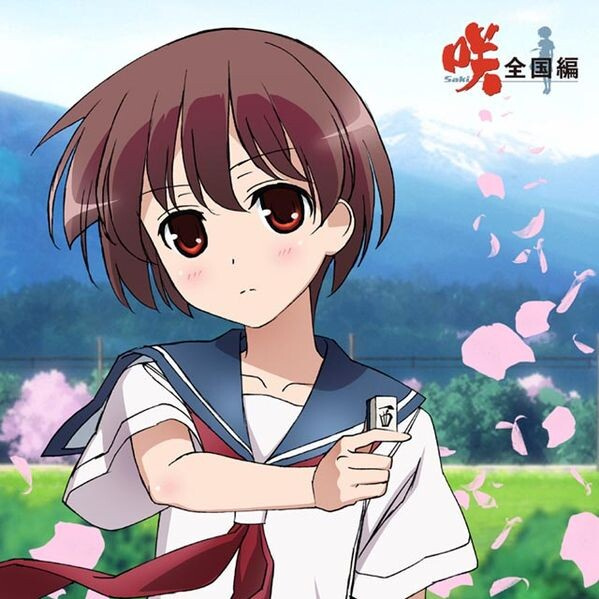
\includegraphics[width=0.3\textwidth]{images/NewSPARKS.jpg}
\quad\quad\quad\quad
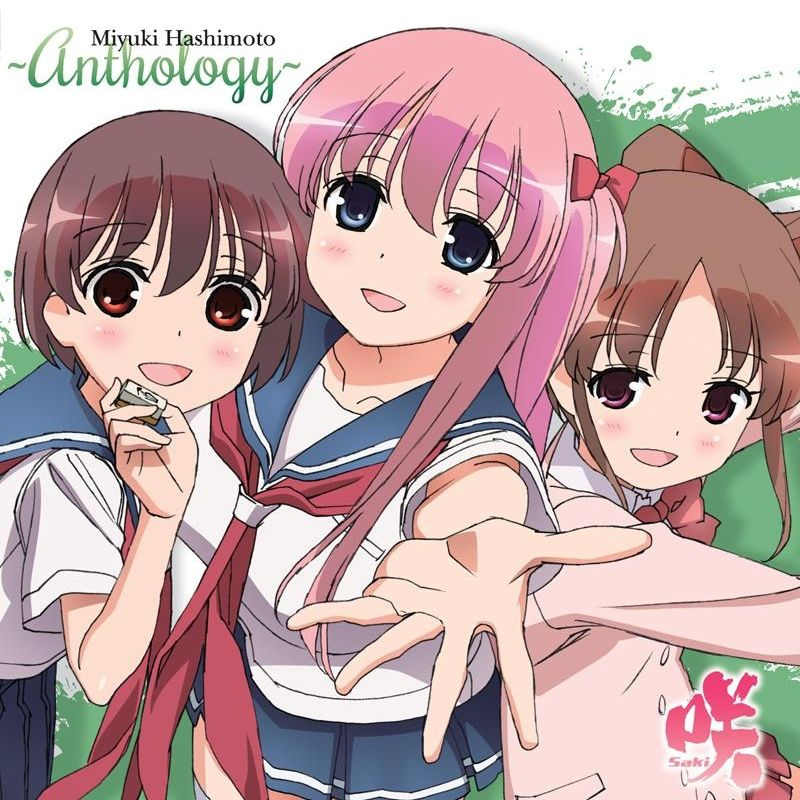
\includegraphics[width=0.3\textwidth]{images/Anthology.jpg}
\end{center}

\newpage

至此,2014日萌本战部分全部结束。\uwave{麻将}以32强占16前无古人的战绩,席卷了这年日萌的半壁江山。\uwave{圆脸}五色全部无压力入围。\uwave{电磁}两名依然在坚挺。\uwave{LL}除\uline{真姬}外全灭。\uwave{春物}、\uwave{点兔}分别在\uwave{圆}\uwave{麻}、\uwave{电}\uwave{L}的支持下挺进两位。\uwave{黄金拼图}在运营的保护下晋级两位。\uline{东山}角色总共五位,全部晋级,其中\uline{千棘}是24强最弱,\uline{花音}是32强最弱。

{\zihao{6}\mincho\ctexset{space=true}
\begin{longtable}{lllll}
 & \toppanb キャラ & \toppanb 作品 & \toppanb 声優 & \\\hline
1 & 高鴨穏乃 & \Saki & 悠木碧 & \\\hline
2 & 宮永咲 & \Saki & 植田佳奈 & \\\hline
3 & 原村和 & \Saki & 小清水亜美 & \\\hline
4 & 佐倉杏子 & \Madomagi & 野中藍 & \\\hline
5 & 初春飾利 & \Railgan & 豊崎愛生 & \\\hline
6 & 鹿目まどか & \Madomagi & 悠木碧 & \\\hline
7 & 清水谷竜華 & \Saki & 石原夏織 & \\\hline
8 & 新子憧 & \Saki & 東山奈央 & \\\hline
9 & 暁美ほむら & \Madomagi & 斎藤千和 & \\\hline
10 & 巴マミ & \Madomagi & 水橋かおり & \\\hline
11 & 松実玄 & \Saki & 花澤香菜 & \\\hline
12 & 御坂美琴 & \Railgan & 佐藤利奈 & \\\hline
13 & 天江衣 & \Saki & 福原香織 & 復活 \\\hline
14 & 美樹さやか & \Madomagi & 喜多村英梨 & \\\hline
15 & 九条カレン & きんいろモザイク & 東山奈央 & \\\hline
16 & 雪ノ下雪乃 & やはり俺の青春ラブコメはまちがっている。 & 早見沙織 & 復活 \\\hline
17 & 園城寺怜 & \Saki & 小倉唯 & 復活 \\\hline
18 & アリス・カータレット & きんいろモザイク & 田中真奈美 & \\\hline
19 & 愛宕洋榎 & \Saki & 松田颯水 & \\\hline
20 & 末原恭子 & \Saki & 寿美菜子 & \\\hline
21 & 神代小蒔 & \Saki & 早見沙織 & \\\hline
22 & 由比ヶ浜結衣 & やはり俺の青春ラブコメはまちがっている。 & 東山奈央 & 復活 \\\hline
23 & 西木野真姫 & ラブライブ! & Pile & \\\hline
24 & シャロ(桐間紗路) & ご注文はうさぎですか? & 内田真礼 & \\\hline
25 & 松実宥 & \Saki & MAKO & 復活 \\\hline
26 & チノ(香風智乃) & ご注文はうさぎですか? & 水瀬いのり & 復活 \\\hline
27 & 大星淡 & \Saki & 斎藤千和 & \\\hline
28 & 愛宕絹恵 & \Saki & 中津真莉子 & \\\hline
29 & 辻垣内智葉 & \Saki & 日笠陽子 & \\\hline
30 & 桐崎千棘 & ニセコイ & 東山奈央 & \\\hline
31 & 宮永照 & \Saki & 中原麻衣 & 復活 \\\hline
32 & 中川かのん(アポロ) & \Kaminomi & 東山奈央 & 復活 \\\hline
\end{longtable}
}

\chapter{季后赛}

\section{10/28(火) プレーオフ抽選}

这次的分组,依然是依靠程序,随机产生的。经过验证,抽签程序没有问题,抽签流程也无不公。这个抽选结果是可信的随机结果。今年季后赛的分组有这样的特征,首先是24强分成8组,然后把复活赛的8个分插到这8组中,每组投一人,取前二位晋级。而决赛圈分组也与季后赛晋级顺位有关系——分别打乱第一位和第二位晋级的,即一位必将遭遇二位的较差淘汰赛,这意味着季后赛中拿到首位的基本上锁定了八强。也因此,阵营主力要尽量争取首位晋级,以便不与其他主力在八强争夺赛中相撞而失去八强,晋级顺位显得十分重要。

分析一下这次的分组,上半区显然是\uwave{麻将}的天下,\uwave{电磁}和\uwave{LL}是被砍死的命运无足为虑,\uwave{春物}\uwave{点兔}也因为是\uwave{圆}\uwave{麻}一手带上来的不会产生威胁,上半区共10个\uwave{麻将}。

下半区是\uwave{圆}\uwave{麻}\uline{东}的大混战,五个\uwave{圆脸}和五个\uline{东山}全部分在了下半区,并且产生了两最强对两最弱的分组,以及\uwave{圆}\uwave{麻}电三家主力对轰的组,\uwave{圆}\uwave{麻}遇到了\uwave{黄图}主力,\uwave{圆脸}遇到了\uline{蓝}\uline{黑}撞分组——这样的场景对三家都是不利且互相制约的。

在\uline{运营}厨\uwave{黄图}的情况下,为了确保萌王不落\uwave{黄图}之手,\uwave{圆}\uwave{麻}决定联手。这时的\uwave{麻将}阵营,\uline{自由}仍有一定权力,对\uwave{黄图}置两可态度;而\uline{末原}则坚持上半区保二\uwave{麻}并且下半场不给\uwave{黄图}活路。\uwave{圆脸}惧于最后一次失去\uline{蓝毛},表示上半区帮助\uwave{麻将}。\uwave{电磁}由于主力\uline{炮姐}和\uwave{圆}\uwave{麻}相撞,尝试向\uwave{圆脸}表示保送\uline{黑焰}萌王以换取\uline{美琴}八强。

整个季后赛八场比赛,由于砍票的原因,持续了一个月多,赛程被割裂。砍票也彻底地变成了意识流砍票,完全毁灭了日萌的公平性。期间,\uwave{电磁}和\uwave{LL}阵营彻底退出日萌赛场并展开了自己的总结,\uwave{圆}\uwave{麻}反\uwave{黄图}联盟形成,\uline{东山}阵营刚刚显现便因为分组遭到摧残而迅速消匿。日萌彻底陷入泥潭。

\newpage

{\zihao{6}\mincho\ctexset{space=true}
\begin{longtable}{|l|r|r|}\hline\hline
\multicolumn{1}{|c|}{\toppanb 10/30(木) FL1組} & \kai 砍票前 & \kai 砍票后 \\\hline
アリス・カータレット@きんいろモザイク & 84 & 80 \\\hline
大星淡@\Saki & 144 & 74 \\\hline
愛宕絹恵@\Saki & 8 & 8 \\\hline
園城寺怜@\Saki & 162 & 87 \\\hline\hline
\multicolumn{1}{|c|}{\toppanb 10/31(金) FL2組} & & \\\hline
清水谷竜華@\Saki & 148 & 108 \\\hline
原村和@\Saki & 190 & 145 \\\hline
西木野真姫@ラブライブ! & 224 & 73 \\\hline
松実宥@\Saki & 10 & 10 \\\hline\hline
\multicolumn{1}{|c|}{\toppanb 11/01(土) FL3組} & & \\\hline
高鴨穏乃@\Saki & 181 & 127 \\\hline
初春飾利@\Railgan & 16 & 12 \\\hline
末原恭子@\Saki & 165 & 108 \\\hline
チノ(香風智乃)@ご注文はうさぎですか? & 79 & 77 \\\hline\hline
\multicolumn{1}{|c|}{\toppanb 11/02(日) FL4組} & & \\\hline
松実玄@\Saki & 174 & 87 \\\hline
シャロ(桐間紗路)@ご注文はうさぎですか? & 56 & 55 \\\hline
神代小蒔@\Saki & 154 & 81 \\\hline
雪ノ下雪乃@やはり俺の青春ラブコメはまちがっている。 & 56 & 44 \\\hline\hline
\end{longtable}
\begin{longtable}{|l|r|r|}\hline\hline
\multicolumn{1}{|c|}{\toppanb 11/04(火) FL5組} & \kai 砍票前 & \kai 砍票后 \\\hline
宮永咲@\Saki & 475 & 206 \\\hline
桐崎千棘@ニセコイ & 39 & 33 \\\hline
鹿目まどか@\Madomagi & 360 & 191 \\\hline
中川かのん(アポロ)@神のみぞ知るセカイ 女神篇 & 37 & 21 \\\hline\hline
\multicolumn{1}{|c|}{\toppanb 11/05(水) FL6組} & & \\\hline
御坂美琴@\Railgan & 489 & 26 \\\hline
新子憧@\Saki & 467 & 173 \\\hline
佐倉杏子@\Madomagi & 451 & 190 \\\hline
天江衣@\Saki & 34 & 13 \\\hline\hline
\multicolumn{1}{|c|}{\toppanb 11/06(木) FL7組} & & \\\hline
九条カレン@きんいろモザイク & 153 & 117 \\\hline
巴マミ@\Madomagi & 315 & 116 \\\hline
愛宕洋榎@\Saki & 18 & 10 \\\hline
宮永照@\Saki & 237 & 106 \\\hline\hline
\multicolumn{1}{|c|}{\toppanb 11/07(金) FL8組} & & \\\hline
美樹さやか@\Madomagi & 119 & 65 \\\hline
辻垣内智葉@\Saki & 15 & 13 \\\hline
暁美ほむら@\Madomagi & 224 & 131 \\\hline
由比ヶ浜結衣@やはり俺の青春ラブコメはまちがっている。 & 24 & 21 \\\hline\hline
\end{longtable}
}

\newpage

\section{10/30(木) FL1}

\VoteTables{
 投票数:398レス\\
 1位 162票 園城寺怜\\
 2位 144票 大星淡\\
 3位 84票 アリス\\
 4位 8票 愛宕絹恵
}{
 投票数:249レス 発行コード数:552\\
 1位 87票 園城寺怜@\Saki\\
 2位 80票 アリス·カータレット@きんいろモザイク\\
 3位 74票 大星淡@\Saki\\
 4位 8票 愛宕絹恵@\Saki
}

\CTEXnoindent
\begin{tabular}{lr}
{\begin{minipage}{0.6\textwidth}\CTEXindent
季后赛看似正常地开幕了,\uwave{麻将}联手\uwave{圆脸}制定了「清场」政策——即16强尽量排除掉其他角色,强行让\uline{运营}从\uwave{圆}\uwave{麻}之中选择萌王。这个政策可以说是\uline{末原}为了防止\uline{运营}强行黑幕而做出的强硬手段,而在\uline{自由}看来,清场政策并不能很顺利地进行,比赛不会过早地进入\uwave{圆}\uwave{麻}垄断时期。事实上,在季后赛时期,\uline{运营}依然是拥有很大权力的,并且此时\uwave{电磁}和\uwave{LL}并未完全退场,不能保证他们不会插手新番,从而导致清场政策执行不成。\\[1em]

1030 三\uwave{麻}围\uwave{黄图}。\uwave{麻将}和\uwave{黄图}应援也都非常丰富,这造成了一定的舆论影响。有热心的朋友在票楼放了很多应援图
% \footnote{原地址:\url{http://saimoe.thread.jp/test/read.cgi/ast/1414169863/754-823}。}
,这个四格漫画也是非常有趣地描述了这场的情况。

\uwave{麻将}尝试执行「清场」政策,在这里表现为「双保」。\uline{托奇}作为前任萌王,是必然要保的;\uline{笨淡}和\uline{爱妹}的抉择则是由于\uline{笨淡}有蜜而\uline{爱妹}没有的缘故(中之人也同样悲剧)。\uline{爱宕绢惠}由于决定好了弃保,本土也表示了同意,所以个位数的的票数也丝毫不意外,甚至这8票中有6票都是海外的多重票。\uwave{麻将}本土保持了优秀的素质,这也在后面的几场弃保中明显表现了出来。很显然,\uwave{麻将}的票力即使双保也不是问题——但是\uwave{麻将}说了不算。

赛中显然出现了来自海外投给\uline{爱丽丝}的多重票,这给\uline{运营}砍赢\uline{爱丽丝}做好了铺垫。于是可爱新番大\uwave{黄图}被顺理成章地砍到二位晋级。这场因为备用投票版临时出现了问题,所以导致第一次集计结果错误,被认为是\uline{运营}砍票把\uline{爱丽丝}砍多了,实际上不是的。相对的,被砍死的\uwave{麻将}则是二位的\uline{大星淡},成为了\uwave{麻将}第一个被砍死的角色。不过\uline{运营}还是不敢操刀过激,还是给了\uwave{麻将}一个首位。
\end{minipage}}
&
% \begin{wrapfigure}[30]{r}[3em]{.45\textwidth}
{\begin{minipage}{.4\textwidth}
 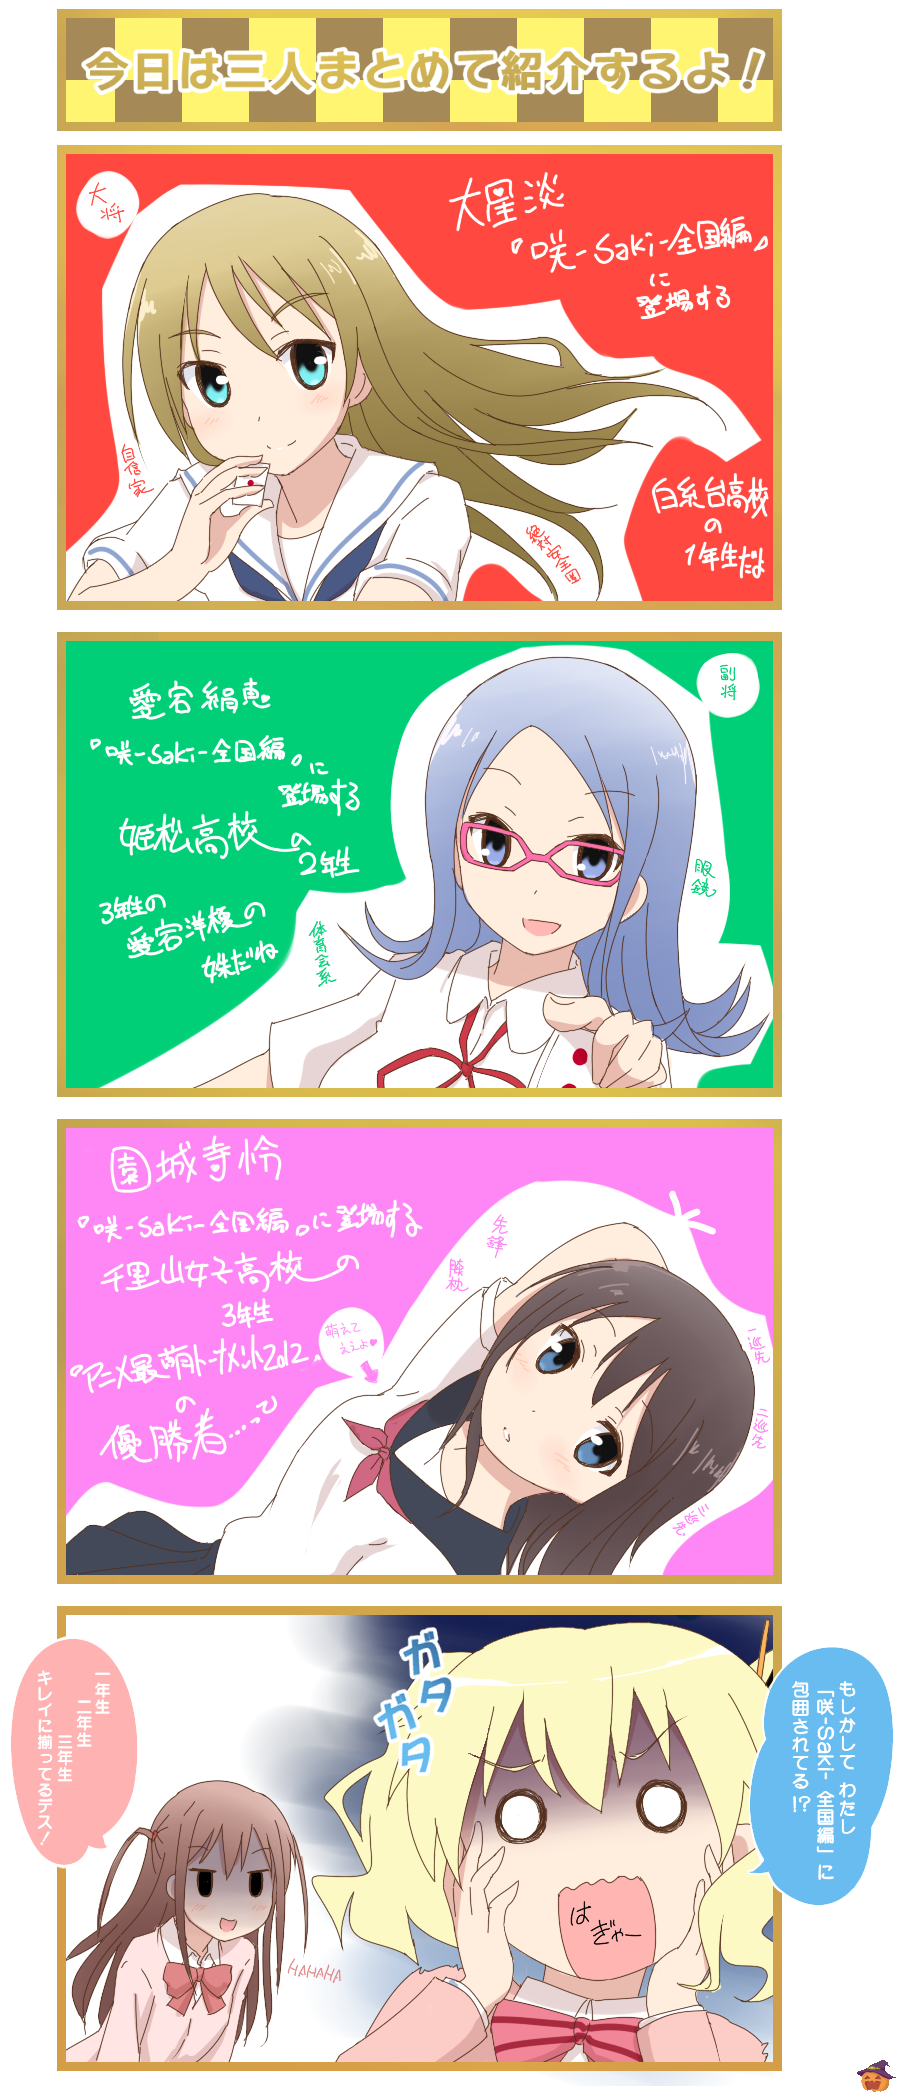
\includegraphics[width=\textwidth]{images/u6566.png}
\end{minipage}}
% \end{wrapfigure}
\end{tabular}
\CTEXindent

\uwave{麻将}被砍死,完全在意料之中,过于贪心毕竟要受到惩罚。这场比赛中乱入投\uline{爱丽丝}的海外厨,表示了对\uwave{麻将}的嘲讽——但是\uwave{麻将}却毫不在意。在\uline{运营}依然拥有话语权的现在,\uline{自由}作为\uwave{麻将}领袖对局势有着自信,预料到了\uwave{黄图}被强行砍赢的结果,并且通过这一次砍票重新树立了在\uwave{麻将}群中的领导地位;\uline{末原}的清场政策开场遭到了挫败也是不可避免的。

\section{10/31(金) FL2}

\VoteTables{
 投票数:572レス\\
 1位 224票 西木野真姫\\
 2位 190票 原村和\\
 3位 148票 清水谷竜華\\
 4位 10票 松実宥
}{
 投票数:336レス 発行コード数:829\\
 1位 145票 原村和@\Saki\\
 2位 108票 清水谷竜華@\Saki\\
 3位 73票 西木野真姫@ラブライブ!\\
 4位 10票 松実宥@\Saki
}

1031 则是\uwave{麻将}和\uwave{LL}之间最后一场斗争了,由于两家早已闹翻,所以这场完全没有外交就硬碰硬地上了——\uwave{麻将}依然是双保,而\uwave{LL}无疑力保\uline{真姬}。\uwave{LL}破天荒地拿出了强烈的斗志,开场一小时后便反超\uwave{麻将}确立了领先优势。由于\uline{真姬}的票多重票特征明显很容易被砍,这也是\uwave{LL}最后一次出场,\uwave{麻将}索性放任了\uline{真姬}的全天领先,「至少让他们面票领先享受一下这个过程」。最后\uline{真姬}顺利达成了首位。

但是结局又是很容易预料的,\uwave{LL}被砍死了。\uwave{LL}此次拼尽了全力,实票220+,战胜了分票的\uwave{麻将};但是运营早已认准了\uwave{LL}这个超多重阵营,下手也是非常不留情。随着\uline{真姬}被砍到两位数,\uwave{LL}阵营也正式退出了今年的日萌赛场。

\uwave{麻将}精神领袖\uline{原村和}再次突破胜场纪录,去年战绩最好的\uline{清水谷龙华}也顶住了分票压力晋级,至于\uline{松实宥}则成为了双保政策的牺牲品。海外\uwave{麻将}再一次为本土\uwave{麻将}的弃保坚定赞叹不已。

\section{11/01(土) FL3}

\VoteTables{
 投票数:441レス\\
 1位 181票 高鴨穏乃\\
 2位 165票 末原恭子\\
 3位 79票 香風智乃\\
 4位 16票 初春飾利
}{
 投票数:324レス 発行コード数:597\\
 1位 127票 高鴨穏乃@\Saki\\
 2位 108票 末原恭子@\Saki\\
 3位 77票 チノ(香風智乃)@ご注文はうさぎですか?\\
 4位 12票 初春飾利@\Railgan
}

双保政策依然在继续,1101 正好只有两个\uwave{麻将},就没所谓弃保了。\uwave{圆脸}作为\uline{UMB}厨,这场给\uline{鸭子}贡献了一些票数。

\uwave{电磁}则直接放弃了\uline{花环}——而三回战的时候她还有500票,这直接向\uline{运营}表示了\uwave{电磁}是彻彻底底的多重,也为后来砍死\uline{炮姐}做好了预演。

至于\uline{智乃},虽然依然有来自海外的多重票,但是70+的票数给\uline{运营}造成了散票有这么多的印象。砍票结果没有改变顺位,因为\uline{运营}实在发现怎样也砍不死\uwave{麻将}了,\uwave{麻将}顺利保送\uline{鸭子}和\uline{恭子}。

\section{11/02(日) FL4}

\VoteTables{
 投票数:440レス\\
 1位 174票 松実玄\\
 2位 154票 神代小蒔\\
 3位 56票 桐間紗路\\
 3位 56票 雪ノ下雪乃
}{
 投票数:267レス 発行コード数:610\\
 1位 87票 松実玄@\Saki\\
 2位 81票 神代小蒔@\Saki\\
 3位 55票 シャロ(桐間紗路)@ご注文はうさぎですか?\\
 4位 44票 雪ノ下雪乃@やはり俺の青春ラブコメはまちがっている。
}

1102 吃到了甜头的\uwave{麻将},继续着双保政策的实施。\uline{龙王}和\uline{公主}的顺位也是显而易见,\uwave{麻将}打得几乎毫无压力。即便是砍票之后,\uwave{麻将}也是保住了两个晋级名额,达成了上半场的一定胜利。

今年把\uwave{春物}厨上来的是\uwave{圆脸},而由于\uwave{圆}\uwave{麻}达成了联盟,所以\uwave{圆脸}也只是在不影响\uwave{麻将}的情况下为\uline{雪乃}投出了一定的多重。所以可以看到在砍票前的三位平票,变成了四位。虽然也很惋惜\uline{雪乃}的退场,但是散票多少也很明显了——没有大阵营支持,怎么可能进入季后赛呢;没有大阵营的继续支持,又怎么继续往下走呢?

\section{11/04(火) FL5}

\begin{longtable}{ll}
\begin{minipage}[t]{.45\textwidth}\kasho
現実の修行の山路も、\\
有為の奥山も越え、\\
その先にいる深山幽谷の化身——\\[.3em]
その\ruby{し}{ま}\ruby{ず}{ど}\ruby{の}{か}を相手にして、\\
嶺の上で花は咲くのか
\end{minipage} &
\begin{minipage}[t]{.45\textwidth}\kai
 超越了现实世界的修行山路,\\
 超脱了诸行无常的苦难生途,\\
 伫立于前方的正是深山幽谷的化身——\\[.3em]
 以这样的\ruby{稳}{圆}\ruby{乃}{香}为对手,\\
 高岭之上鲜花是否还能绽放呢
\end{minipage}
\end{longtable}

1104 是真正意义上的\textbf{第一次\uwave{圆}\uwave{麻}大战}。达成「神圣联盟」的\uwave{圆}\uwave{麻}阵营,终于产生了第一次正面对撞。

\begin{longtable}{ll}
\begin{minipage}[t]{.34\textwidth}\kai 砍票前:\\\VoteFont
 投票数:911レス\\
 1位 475票 宮永咲\\
 2位 360票 鹿目まどか\\\\
 3位 39票 桐崎千棘\\
 4位 37票 中川かのん
 \end{minipage} &
\begin{minipage}[t]{.62\textwidth}\kai 砍票后:\\\VoteFont
 投票数:451レス 発行コード数:994\\
 1位 206票 宮永咲@\Saki\\
 2位 191票 鹿目まどか@\Madomagi\\
 3位 33票 桐崎千棘@ニセコイ\\
 4位 21票 中川かのん(アポロ)@\Kaminomi
\end{minipage}
\end{longtable}

有人要问了,既然是取前两位晋级,那么为什么要争个你死我活呢?原因一个是决赛圈的交叉淘汰赛制,\uwave{麻将}需要防止\uline{咲}\uline{和}相撞导致阵营分裂;一个是\uline{宫永咲}代表了《咲-Saki-》这一作品的名字,而\uline{鹿目圆香}则代表了《\Mado》这一作品的名字,这一战可以说是两个阵营堵上作品名的荣誉之战。\uwave{圆}\uwave{麻}的这一场荣誉之战,可以说谁赢了谁就能够拿到萌王,这毫不夸张,并且后来的事实也证实了这一说法。

这次\uwave{麻将}可是做好了十足的做准备跟有着不败传说的\uwave{圆脸}好好干上一仗。开场\uwave{麻将}就确立了领先优势,但是\uwave{圆脸}也不甘落后,整个白天都在坚持追赶,一度拉近了票差,下午几乎追平。\uwave{麻将}则一直在尽力压制着\uwave{圆脸},维持到了海底时间,又是一波爆票把票差迅速拉开,并且达成了百票杀。统计下来,\uwave{圆}\uwave{麻}两家大战,票尾一个也没红——这又一次说明了\uwave{圆}\uwave{麻}的票源并非是服务器。当然还有更有意思的统计,就是两家的萌文显然已经严重不够用了,赛场上出现了大量的重复萌文。也可以看到,依赖于人工的\uwave{圆脸}在半夜的出票率要少于自动化的\uwave{麻将}。\uwave{麻将}第一次完成了对\uwave{圆脸}的胜利。

这次砍票直到1110才完成。砍票之后的结果,没有顺位变化。但是可以注意到,显著的百票差被砍成了15票差。这个显然是运营有意而为之——强行形成\uwave{圆}\uwave{麻}不相上下的印象。可以透露这次的\uwave{麻将}有78张散票,至于运营怎么意识流砍出来一片天的,就不得而知了。总之,\uline{岭上大魔王}为\uwave{麻将}开了个好头,\uwave{圆脸}的最强神话就此破灭。贴吧和2ch的\uwave{麻}蜜也逐渐开始关注今年的比赛。

四个人比赛,为啥光说\uwave{圆}\uwave{麻}呢?因为剩下这俩,过于杂鱼。之前也提到过,论战绩,\uline{桐崎千棘}是24强最弱,\uline{中川花音}则是32强最弱,无论遇到谁都没有胜出机会,何况是两最弱对两最强,可以完全等死了。另一方面,今年的\uline{东山}阵营,是由\uwave{麻将}领袖\uline{自由}一手带起来的,并有着\uwave{圆脸}团长\uline{兰博},以及另一位大厨\uline{团子}的支持。\uline{千棘}能够晋级,得益于\uwave{圆脸}的连记;\uline{花音}能够复活,在于\uwave{麻将}的力保。这样,两家在为自己的角色打得火热的时候,没有太多的余力去照顾\uline{东山}。即便是\uline{自由},也只是拿出了30票去支援了\uline{东山}两位角色,\uline{花音}20\uline{千棘}10——倒也说明运营砍得「比例」蛮精准的。已经不会再有出场机会的\uline{中川花音},完成了她的谢幕之战,拿到了历史最佳战绩,宣告了\uwave{神知}退出历史舞台,这也照应了现实中\uline{东山奈央}正式从\uline{中川花音}毕业。总之,昙花一现的\uline{东山}阵营就此一下子失去了两位大将。

\section{11/05(水) FL6}

请记住这张曲线,它记录了\uline{御坂美琴}在2014日萌中最为精彩的演出。

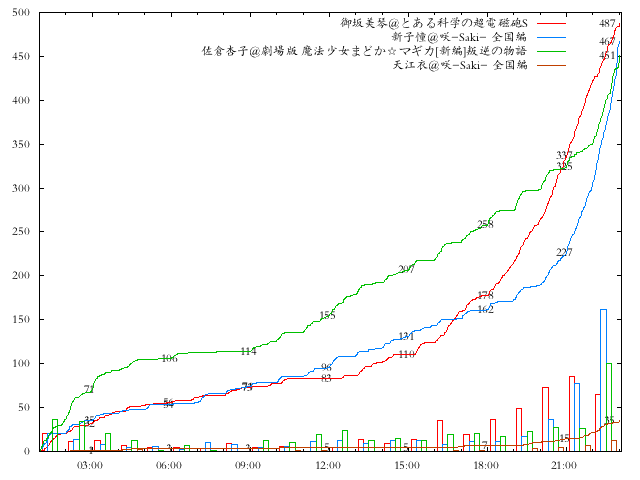
\includegraphics[width=.6\textwidth]{images/graph1105.png}

\VoteTables{
 投票数:1441レス\\
 1位 489票 御坂美琴\\
 2位 467票 新子憧\\
 3位 451票 佐倉杏子\\
 4位 34票 天江衣
}{
 投票数:402レス 発行コード数:1545\\
 1位 190票 佐倉杏子@\Mado\\
 2位 173票 新子憧@\Saki\\
 3位 26票 御坂美琴@\Railgan\\
 4位 13票 天江衣@\Saki
}

1105 的比赛应该分成两个时期,一个是实票时期,一个是砍票时期。我们先来说说今年最激烈的这场实票大战。从数据上可以看到,这场比赛发行1500,投出1400,发行量非常之大,甚至超过了2010年的水平;投出比也是前所未有的高,可以见到三大阵营都在浴血奋战。第二次\uwave{圆}\uwave{麻}大战加上第四次\uwave{电}\uwave{麻}大战,就是这场\uwave{圆}\uwave{麻}\uwave{电}主力的最巅峰决战。

惨败给\uwave{麻将}的\uwave{圆脸}吃一堑长一智,开场迅速确立了优势。而这时,\uwave{麻将}和\uwave{电磁}都掉了链子——\uwave{麻将}的调度中心服务器网络中断,又部署了一台新机器,从而失去了开场约的大部分票;\uwave{电磁}则因为有主力的电脑硬盘损坏,一定程度上失去了开场约票优势。可以看到,\uwave{麻将}和\uwave{电磁}开场简直惨不忍睹,而\uwave{圆脸}则持续追击,前三个小时一直在爆票,拉开了相当大的优势,并维持到了白天。\uwave{麻将}则开始和\uwave{电磁}纠缠在了一起不分上下,直到中午\uwave{电磁}稍有松懈,\uwave{麻将}才终于把票差拉开,而此时\uwave{圆脸}依然在稳定地涨票。
晚饭时间到了,爆票开始了,然而这次爆票的不是\uwave{麻将},而是\uwave{电磁}。\uwave{电磁}开始了爆票并迅速追上了\uwave{麻将}完成了反超,稍作停顿后,开始了均匀的海底爆票。\uwave{麻将}给与了\uwave{电磁}反超的机会,把抛物线爆票推后到了八点。这时,\uwave{电磁}迅速缩小了和\uwave{圆脸}的差距,实现了反超,并很快将\uwave{圆脸}甩在了后面。\uwave{圆脸}则被形势所逼产生了严重的阶梯爆票,不得不在最后一小时开始了直线爆票。\uwave{麻将}则维持着曲线开始了最后一小时的惊天爆票——\uline{新子憧}借助\uline{天江衣}的海底之力足足爆出了160+,并在最后几分钟完成了对\uwave{圆脸}的反超达成了二位。\uwave{电磁}维持着胜利达成了首位,\uwave{圆脸}则不得不屈居第三。开场的顺位被完全打破,三次反超也成为了日萌史上的经典。

这一组,死亡之组。\uwave{电磁}的唯一主力\uline{炮姐}\uline{御坂美琴},竟然分给了\uwave{圆}\uwave{麻}的主力。\uwave{圆脸}准萌的\uline{红毛}\uline{佐仓杏子}出战;\uwave{麻将}则是「\uline{咲衣和稳憧}」五大主力之二的冲突——\uline{新子憧}和\uline{天江衣}。当时分组一出,可以说\uline{自由}整个心都碎了,\uwave{麻}蜜一片哀嚎。
\uline{天江衣},日萌有过八强,度萌也和\uline{宫永咲}内战获得了四强;而\uline{新子憧},组决惜败于\uline{原村和},身交\uline{东山}和\uwave{麻将}两个阵营——于是弃保就决定了。本土同样决定了这一弃保,并张贴了弃保告知,海外和本土依然达成了一致。然而海外并没有彻底抛弃\uline{天江衣},不仅在票力紧张的情况下为\uline{天江衣}继续投票,还在海底时间用\uline{小衣}的AA图为\uline{ako}应援。
「\uline{天江}已逝,只为\uline{新子}。」可惜的是,因为\uwave{麻将}开场没能领先,被砍成二位的命运已经注定,此时\uwave{麻将}已经做好了「\uline{憧}不八」的准备。\uwave{电磁}则因为同样出了问题,没能够拿到今年的最高票。

剩下的就是运营的大刀舞台了。正当运营砍得欢快的时候,1111就在光棍节当天,\uline{RUN}的电脑终于被大厨诅咒得爆炸了。
这场比赛终于在1124 \uline{RUN}买来新电脑之后砍完了,日萌日程也因此延迟了一个月……
\uline{运营}砍了一刀又一刀,这一刀一刀的,犹如给大厨实千刀万剐之刑,生不犹死。

最惨的是\uline{炮姐},活生生从近500票砍到了26票,酿成了最严重的砍票案,所以我们形容\uline{炮姐}之死是「惨死」于\uline{运营}之手。\uwave{电磁}阵营彻底退出日萌战场,「\uline{炮}不八」传说继续。\uwave{电磁}阵营的努力我们有目共睹,虽败犹荣。

杏子被砍到了首位,然而\uwave{圆脸}怎么也高兴不起来。\uline{ako}二位则意味着大概率撞到主力,也注定了「\uline{憧}不八」的结局。三个阵营有着不同的胜负,不同的荣光,不同的屈辱,全在一场之内表现了出来。

\section{11/06(木) FL7}

\VoteTables{
 投票数:732レス\\
 1位 315票 巴マミ\\
 2位 237票 宮永照\\
 3位 153票 九条カレン\\
 4位 18票 愛宕洋榎
 }{
 投票数:349レス 発行コード数:1049\\
 1位 117票 九条カレン@きんいろモザイク\\
 2位 116票 巴マミ@\Mado\\
 3位 106票 宮永照@\Saki\\
 4位 10票 愛宕洋榎@\Saki
}

三家合战之后,\uwave{麻将}内部发生了严重的争吵。\uline{自由}依然有着\uline{东山}厨的思维,坚持保送\uline{可怜},试图通过和\uline{运营}合作,来达成对\uwave{圆脸}的战略威胁;而\uline{末原}惧于\uline{可怜}因此成为萌王,断送\uline{乳和}前程,认为可怜是核武器一样的存在,反对保可怜。

事实证明两个人都错了:\uline{自由}认识到了如果\uwave{麻将}支援,\uline{可怜}必然会被砍成首位晋级,但是错估了\uline{运营}会砍死\uwave{圆脸};\uline{末原}的清场政策一开始就是错误的,并遭到了\uline{运营}的粉碎,但是其认为\uwave{黄图}作为大规模杀伤性武器的威力则被验证了。

1106 \uline{自由}坚持为\uline{可怜}投票,\uwave{麻}群内部终于达成了妥协。开场了,\uline{可怜}和\uline{洋榎}的票出了出来——然而更严重的问题来了——本土意志是\uline{照姐}!海外经过连续两天的苦斗,没能够即使去讨论串查看舆情。结果本土意志是\uline{照姐},海外意志是\uline{爱姐}。本土\uwave{麻}领袖(姑且这么认为)\uline{まこ厨}在投票楼用日语、汉语、汉语拼音、英语、AA图一直在嚷着「请投\uline{宫永照}」。\uline{自由}发现之后,认识到了问题的严重性,立即作出决定停止投票,改投\uline{宫永照}。然而这时\uwave{麻将}完全没有\uline{照姐}的萌文,于是大家发起了十二分的努力,为\uline{照姐}凑出来一堆萌文,终于保起来\uline{照姐}。\uline{自由}则在票楼直接以多重屋的身份向本土表示道歉,并表示了保\uline{可怜}的想法;本土做出了回应,表示支持多重屋的决定,但是「如果投\uwave{麻将}的话还请投\uline{宫永照}」。这样,海外与本土之间的第一次联系成立,双方随后达成了一系列共识。

\uwave{麻将}没有意愿争夺首位,因为本来\uline{照姐}就不是预定要保的;\uline{洋榎}除了开场的几票之外再没怎么涨过票。相对的,\uline{自由}对于有着\uline{东山}身份的\uline{九条可怜}十分热衷,顶着群内压力一直在推\uline{可怜},但也只能推到百余票。\uline{学姐}首位毫无压力。

接下来就是延期一个月的砍票。\uline{运营}非常「巧合」地砍成了「\uwave{黄图}=\uwave{圆脸}+1」「\uwave{圆脸}=\uwave{麻将}+\uwave{麻将}」的结果。强行「\uwave{圆}=\uwave{麻}」也是醉醉的。\uline{照姐}被砍死,跟随\uline{笨淡}一起去了。\uwave{黄图}一票杀\uwave{圆脸}跃于首位,不知道该笑还是该哭。
\newpage
\section{11/07(金) FL8}

\VoteTables{
 投票数:約382レス\\
 1位 224票 暁美ほむら\\\\
 2位 119票 美樹さやか\\\\
 3位 24票 由比ヶ浜結衣\\\\
 4位 15票 辻垣内智葉
 }{
 投票数:230レス 発行コード数:約400\\
 1位 131票 暁美ほむら@\Madomagi\\
 2位 65票 美樹さやか@\Madomagi\\
 3位 21票 由比ヶ浜結衣@やはり俺の青春ラブコメはまちがっている。\\
 4位 13票 辻垣内智葉@\Saki
}

1107 是季后赛最没意思的一场。\uwave{麻将}出场了一个杂鱼得无以复加的杂鱼,完全是因为「对手太弱」上来的。而春物兼\uline{东山}阵营的\uline{结衣},则因为\uwave{圆}\uwave{麻}联盟的友好互不侵犯协议,没人敢给\uline{结衣}投票。\uline{晓美焰}倍杀\uline{美树沙耶香}的剧本,应该是\uwave{圆脸}强烈保\uline{焰}的意志所造成的。

开场本土\uwave{麻将}尝试在票楼联络海外多重屋,希望能够弃掉\uline{辻垣内智叶},号召\uwave{麻将}阵营为\uline{由比滨结衣}投票。\uline{自由}表示,海外\uwave{麻将}奋战多日疲惫不堪,希望能够休整一下,准备后面的比赛。本土表示了理解和问候,并呼吁本土\uwave{麻将}本场弃权。大家都没想到的是,这一歇,就歇了一个多月。
\\

下半区「五\uwave{圆}五\uline{东}五\uwave{麻将}」的局势,直接把今年日萌带上了又一个高潮。而这一高潮的结局是\uwave{超电磁炮}阵营的彻底退出,以及\uline{东山}阵营刚崛起就变得名存实亡的后果。
\\[1em]

季后赛结束,全场只剩下三个阵营——\uwave{麻将}、\uwave{圆脸}、\uwave{黄图}。

\uwave{电磁}和\uwave{LL}被\uline{运营}砍出赛场,\uwave{春物}\uwave{点兔}最终没能继续下去,\uline{东山}阵营则幸运留下了两个。

日萌变得有意思而又没意思。
\newpage
\section{11/21(金) 服务器查封案}

由于运营的电脑损坏,日萌赛程暂停了一个多月。这一个多月期间也发生了一些和萌战有关的事情,其中 1121 的服务器查封案直接影响了日萌的最终结果。

日萌暂停,厨群变成了吹水群,就连萌文也懒得准备的大厨们,在11月19日这天得知了一则新闻『日本警方侦破非法中转服务器大案~拟逮捕一二十名中国人』。\uline{自由}不以为然地打开了久违的VNC,发现有几个打不开了。一问,果真是新闻中的日本服务器被查封。21日,所有服务器全部报废。

本来\uwave{麻将}是个穷阵营,一直在担心决赛圈\uwave{圆脸}花钱购置大量服务器来用金钱优势压制\uwave{麻将}——有传说去年\uline{兰博}包了整个机房,当然这不可能就是了。这一封服务器,大家就只能用VG来刷票,就变成了纯粹的抢票大作战。\uline{末原}说「全靠VG躺着赢。」事实上也是这样,因为服务器的完全不可用,导致了技术领先的\uwave{麻将}获得了最终的胜利。

服务器查封的另一后果是\uline{末原}实际领导地位的确立。本来\uline{自由}还拥有服务器的控制权,每日控制曲线和放海底。服务器的不可用,使处在校园网封锁状态连不上VPN的\uline{自由}基本丧失了对比赛的控制权。名义上\uline{自由}依然是\uwave{麻将}领袖,实际上\uline{末原}已经完全掌握了实权。\uline{自由}只有找萌文和编写票面这种杂活儿可干了。(或许还有背黑锅?)

\uline{末原}在这个时期对挖掘机代码做了较大的更新,「挖掘机技术哪家强」的答案也正是\uwave{麻将}。考虑到抢票问题和抓票效率等,\uline{末原}又为挖掘机套上了虚拟化,实现了真正的多线程日萌技术;更新了抢票算法,使\uwave{圆脸}后期每每看到红票叫苦不迭。而本来就有的IP防冲突机制,则让\uwave{麻将}的撞票率降到了最低。将「用电脑编程控制挖掘机炒菜」这一玩笑话变成现实的,正是\uline{末原}。

\uwave{圆脸}也是很早发现了服务器的报废,产生了严重内部动摇。\uwave{电磁}和\uwave{LL}则在最后才知道这一事实。

服务器查封案标志着日萌线路的彻底转向。2014决胜圈的比赛方式发生了巨大变化。

\chapter{决胜赛}

{\zihao{6}\mincho
\begin{longtable}{|l|rccccccc}
\hline
\multicolumn{1}{|c|}{\toppanb キャラクター名} & \multicolumn{1}{c}{} & & \multicolumn{2}{|c|}{\toppanb 準々決勝} & \multicolumn{2}{c|}{\toppanb 準決勝} & \multicolumn{2}{c|}{\toppanb 決勝}\\ \hline
{松実玄@\Saki} & \multicolumn{1}{r|}{357} & \multicolumn{1}{c|}{FT1} & \multicolumn{1}{c|}{松実玄} & \multicolumn{1}{c|}{} & \multicolumn{1}{c|}{} & \multicolumn{1}{c|}{} & \multicolumn{1}{c|}{} & \multicolumn{1}{c|}{}\\ \cline{1-2}
{神代小蒔@\Saki} & \multicolumn{1}{r|}{169} & \multicolumn{1}{c|}{12/13} & \multicolumn{1}{c|}{90} & \multicolumn{1}{c|}{Qf1} & \multicolumn{1}{c|}{原村和} & \multicolumn{1}{c|}{} & \multicolumn{1}{c|}{} & \multicolumn{1}{c|}{}\\ \cline{1-4}
{原村和@\Saki} & \multicolumn{1}{r|}{409} & \multicolumn{1}{c|}{FT2} & \multicolumn{1}{c|}{原村和} & \multicolumn{1}{c|}{12月} & \multicolumn{1}{c|}{398} & \multicolumn{1}{c|}{} & \multicolumn{1}{c|}{} & \multicolumn{1}{c|}{}\\ \cline{1-2}
{新子憧@\Saki} & \multicolumn{1}{r|}{294} & \multicolumn{1}{c|}{12/14} & \multicolumn{1}{c|}{203} & \multicolumn{1}{c|}{17日} & \multicolumn{1}{c|}{} & \multicolumn{1}{c|}{Sf1} & \multicolumn{1}{c|}{原村和} & \multicolumn{1}{c|}{}\\ \cline{1-6}
{佐倉杏子@\Madomagi} & \multicolumn{1}{r|}{328} & \multicolumn{1}{c|}{FT3} & \multicolumn{1}{c|}{佐倉杏子} & \multicolumn{1}{c|}{} & \multicolumn{1}{c|}{} & \multicolumn{1}{c|}{12月} & \multicolumn{1}{c|}{187} & \multicolumn{1}{c|}{}\\ \cline{1-2}
{アリス・カータレット@きんいろモザイク} & \multicolumn{1}{r|}{90} & \multicolumn{1}{c|}{12/13} & \multicolumn{1}{c|}{334} & \multicolumn{1}{c|}{Qf2} & \multicolumn{1}{c|}{美樹さやか} & \multicolumn{1}{c|}{20日} & \multicolumn{1}{c|}{} & \multicolumn{1}{c|}{}\\ \cline{1-4}
{九条カレン@きんいろモザイク} & \multicolumn{1}{r|}{76} & \multicolumn{1}{c|}{FT4} & \multicolumn{1}{c|}{美樹さやか} & \multicolumn{1}{c|}{12月} & \multicolumn{1}{c|}{48} & \multicolumn{1}{c|}{} & \multicolumn{1}{c|}{} & \multicolumn{1}{c|}{}\\ \cline{1-2}
{美樹さやか@\Madomagi} & \multicolumn{1}{r|}{409} & \multicolumn{1}{c|}{12/14} & \multicolumn{1}{c|}{339} & \multicolumn{1}{c|}{18日} & \multicolumn{1}{c|}{} & \multicolumn{1}{c|}{} & \multicolumn{1}{c|}{} & \multicolumn{1}{c|}{Final}\\ \cline{1-8}
{園城寺怜@\Saki} & \multicolumn{1}{r|}{451} & \multicolumn{1}{c|}{FT5} & \multicolumn{1}{c|}{園城寺怜} & \multicolumn{1}{c|}{} & \multicolumn{1}{c|}{} & \multicolumn{1}{c|}{} & \multicolumn{1}{c|}{} & \multicolumn{1}{c|}{12月}\\ \cline{1-2}
{巴マミ@\Madomagi} & \multicolumn{1}{r|}{328} & \multicolumn{1}{c|}{12/13} & \multicolumn{1}{c|}{188} & \multicolumn{1}{c|}{Qf3} & \multicolumn{1}{c|}{高鴨穏乃} & \multicolumn{1}{c|}{} & \multicolumn{1}{c|}{} & \multicolumn{1}{c|}{23日}\\ \cline{1-4}
{高鴨穏乃@\Saki} & \multicolumn{1}{r|}{622} & \multicolumn{1}{c|}{FT6} & \multicolumn{1}{c|}{高鴨穏乃} & \multicolumn{1}{c|}{12月} & \multicolumn{1}{c|}{126} & \multicolumn{1}{c|}{} & \multicolumn{1}{c|}{} & \multicolumn{1}{c|}{}\\ \cline{1-2}
{鹿目まどか@\Madomagi} & \multicolumn{1}{r|}{311} & \multicolumn{1}{c|}{12/14} & \multicolumn{1}{c|}{98} & \multicolumn{1}{c|}{17日} & \multicolumn{1}{c|}{} & \multicolumn{1}{c|}{Sf2} & \multicolumn{1}{c|}{宮永咲} & \multicolumn{1}{c|}{}\\ \cline{1-6}
{暁美ほむら@\Madomagi} & \multicolumn{1}{r|}{356} & \multicolumn{1}{c|}{FT7} & \multicolumn{1}{c|}{暁美ほむら} & \multicolumn{1}{c|}{} & \multicolumn{1}{c|}{} & \multicolumn{1}{c|}{12月} & \multicolumn{1}{c|}{187} & \multicolumn{1}{c|}{}\\ \cline{1-2}
{清水谷竜華@\Saki} & \multicolumn{1}{r|}{435} & \multicolumn{1}{c|}{12/13} & \multicolumn{1}{c|}{432} & \multicolumn{1}{c|}{Qf4} & \multicolumn{1}{c|}{宮永咲} & \multicolumn{1}{c|}{21日} & \multicolumn{1}{c|}{} & \multicolumn{1}{c|}{}\\ \cline{1-4}
{宮永咲@\Saki} & \multicolumn{1}{r|}{521} & \multicolumn{1}{c|}{FT8} & \multicolumn{1}{c|}{宮永咲} & \multicolumn{1}{c|}{12月} & \multicolumn{1}{c|}{297} & \multicolumn{1}{c|}{} & \multicolumn{1}{c|}{} & \multicolumn{1}{c|}{}\\ \cline{1-2}
{末原恭子@\Saki} & \multicolumn{1}{r|}{140} & \multicolumn{1}{c|}{12/14} & \multicolumn{1}{c|}{594} & \multicolumn{1}{c|}{18日} & \multicolumn{1}{c|}{} & \multicolumn{1}{c|}{} & \multicolumn{1}{c|}{} & \multicolumn{1}{c|}{}\\ \hline
\end{longtable}
}

日萌的重头戏本应该是决胜赛圈的,然而由于运营\uline{RUN}拖延了一个多月,观众的热情被逐渐磨退。由于运营的砍票,\uwave{电磁}\uwave{LL}早早退场,只剩下\uwave{圆}\uwave{麻}联盟试图绞杀\uwave{黄图},变成了单纯无战术的硬碰硬。

最终\uline{RUN}在为\uline{晓美焰}砍出八强之后彻底放弃治疗,\uline{uBJ}担当了新运营并在年内完成了比赛。
\\

决胜圈不仅是阵营之间的最终对决,也成为了大厨对运营的挑战。最终不正多重战胜了不正砍票。

\newpage

\section{12/10(水) 決勝T抽選}

{\kasho
\begin{longtable}{lll}
 FT1 & 松実玄@\Saki\\ & 神代小蒔@\Saki\\
 FT2 & 原村和@\Saki\\ & 新子憧@\Saki\\
 FT3 & 佐倉杏子@\Madomagi\\ & アリス·カータレット@きんいろモザイク\\
 FT4 & 九条カレン@きんいろモザイク\\ & 美樹さやか@\Madomagi\\
 FT5 & 園城寺怜@\Saki\\ & 巴マミ@\Madomagi\\
 FT6 & 高鴨穏乃@\Saki\\ & 鹿目まどか@\Madomagi\\
 FT7 & 暁美ほむら@\Madomagi\\ & 清水谷竜華@\Saki\\
 FT8 & 宮永咲@\Saki\\ & 末原恭子@\Saki
\end{longtable}
}

\uline{RUN}因为「电脑坏了」没有将季后赛的票及时砍完,赛程被一再推迟。直到\uline{RUN}声称他买了一台新电脑,砍完了票之后,16强确定,终于可以分组了。

预选、本战、季后赛的抽签,经过验证,运营没有做任何手脚,结果公平公正。而决胜赛的抽选,则不得不怀疑\uline{运营}有了作弊的嫌疑。\uline{RUN}声称自己的电脑无法正常运行抽选程序,表示会使用其他方式比如Excel来完成抽选。

——观众们表示你爱咋咋地,赶快抽选把比赛赶快结束!

——于是\uline{RUN}就真的用Excel来抽选了,结果如上。之后\uline{RUN}把抽选过程录制的视频上传到了YouTube\footnote{决赛抽选视频地址:\url{http://www.youtube.com/watch?v=VZjdAjqQTDs}。}。

这个时候运营楼出现了\uline{uBJ}表示将协助运营工作完成下面的比赛,\uline{RUN}也表示了承认。

分组既出,八强已定,剧本也就写好了。\uwave{圆}\uwave{麻}联盟之前达成了一项约定,无论分组如何,都不允许为\uwave{黄金拼图}投票。\uline{自由}被\uline{末原}限制住,\uline{兰博}也作为团长不得不立场坚定,于是即便是有着\uline{东山}身份的\uline{九条可怜},在\uline{东山}阵营两大头的\uline{自由}和\uline{兰博}都不再支持的情况下,注定了不八命运。

\uwave{麻将}分析了一下情况,计划除\uline{红蓝}之外全部连记死\uwave{圆脸},虽然\uline{红蓝}撞上了\uwave{黄图},但由于\uwave{圆}\uwave{麻}联盟的「君子协定」,如果没有外人插手的情况下基本保送了\uwave{圆脸}——事实上服务器全灭的情况下也没有人能够插手。\uwave{麻将}决定坚决阻击\uline{晓美焰},尽量避免\uline{咲焰}相撞导致的大战。而\uline{憧和}再次相撞,则不得不说「\uline{憧}不八」铁板钉钉。\uline{咲和}正好被分在上下两个半区,\uline{自由}和\uline{末原}的矛盾被推迟到了最后,避免了阵营过早分裂。这个分组对\uwave{麻将}有利也有弊。

\uwave{圆脸}那边也不好过,一个是因为服务器查封案搞得有点虚,一个是\uline{晓美焰}碰上了\uwave{麻将}的\uline{龙怜}连记,怕是又要「\uline{焰}不八」。虽然赛程缩短到了两天完成十六进八,但是这个连记不得不让\uwave{圆脸}叫苦不迭。阵营内部出现了相当严重的动摇,开始考虑主动放弃比赛,试图向\uwave{麻将}议和,弃\uline{黄粉}来换取\uline{黑}八强。

\section{12/13(土) FT1 FT3 FT5 FT7}

\VoteTables{
 投票数:804レス\\
 FT1組\\
 1位 357票 松実玄\\
 2位 169票 神代小蒔\\
 FT3組\\
 1位 328票 佐倉杏子\\
 2位 90票 アリス·カータレット\\
 FT5組\\
 1位 451票 園城寺怜\\
 2位 328票 巴マミ\\
 FT7組\\
 1位 435票 清水谷竜華\\
 2位 356票 暁美ほむら
}{
 投票数:405レス 発行コード数:835\\
 FT1組\\
 1位 166票 松実玄@\Saki\\
 2位 105票 神代小蒔@\Saki\\
 FT3組\\
 1位 170票 佐倉杏子@\Mado\\
 2位 82票 アリス·カータレット@きんいろモザイク\\
 FT5組\\
 1位 210票 園城寺怜@\Saki\\
 2位 175票 巴マミ@劇場版 魔法少女まどか\\
 FT7組\\
 1位 197票 暁美ほむら@\Mado\\
 2位 195票 清水谷竜華@\Saki
}

\Graph{1213c.png}
\Graph{1213d.png}

虽然\uwave{圆脸}考虑了向\uwave{麻将}议和,但是只停留在高层之间的私聊,到了比赛之前的最后一刻都没有拿到正式的谈判场合上去说。——时间不等人,比赛就这么毫不留情地开始了,议和没能进行成,大家都投入到了日萌复赛之后第一场比赛,也是决定\uline{焰}八\uline{焰}不八的重要场次之上。1213是为\textbf{第三次\uwave{圆}\uwave{麻}大战}。

比赛就是比赛,\uwave{麻将}没有给\uwave{圆脸}任何机会,全天领先,狠狠压制着\uwave{圆脸}。\uline{园城寺怜}和\uline{巴麻美}的萌王之战,以\uwave{麻将}的绝对领先宣告结束;而\uline{清水谷龙华}凭借\uline{偷鸡}的「仙人指路」打开外挂,最后近百票杀\uline{晓美焰}。\uline{爱丽丝}面对两家都不连记自己的情况,不足百票。\uline{松实玄}轻松保送,\uline{神代小莳}凭借着神降的幸运走到这里也足够了。

当然,比赛结果不能信。\uline{RUN}两场一起砍,送了\uline{晓美焰}一个八强——不过这2票差真的叫人笑掉大牙。「\uline{焰}不八」的称号竟然以这种方式得以摆脱,大家心里都不舒服。当然,\uwave{麻将}被砍死也是理所当然,真正的散票结果确实是\uline{偷鸡}多于\uline{大腿},\uline{焰}大致领先\uline{龙华}10票差左右,砍得倒也不错。

\section{12/14(日) FT2 FT4 FT6 FT8}

\VoteTables{
 投票数:951レス\\
 FT2組\\
 1位 409票 原村和\\
 2位 294票 新子憧\\
 FT4組\\
 1位 409票 美樹さやか\\
 2位 76票 九条カレン\\
 FT6組\\
 1位 622票 高鴨穏乃\\
 2位 311票 鹿目まどか\\
 FT8組\\
 1位 521票 宮永咲\\
 2位 140票 末原恭子
 }{
 投票数:389レス 発行コード数:977\\
 FT2組\\
 1位 165票 原村和@\Saki\\
 2位 111票 新子憧@\Saki\\
 FT4組\\
 1位 182票 美樹さやか@\Mado\\
 2位 69票 九条カレン@きんいろモザイク\\
 FT6組\\
 1位 206票 高鴨穏乃@\Saki\\
 2位 166票 鹿目まどか@\Mado\\
 FT8組\\
 1位 197票 宮永咲@\Saki\\
 2位 67票 末原恭子@\Saki
}

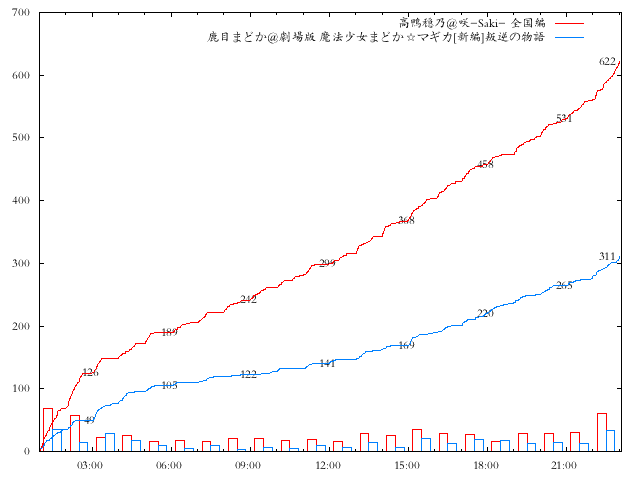
\includegraphics[width=.5\textwidth]{images/graph1214c.png}

1214是为\textbf{第四次\uwave{圆}\uwave{麻}大战}。\uwave{圆脸}吸取了上一场的教训教训,这场早早做好了准备,开场取得了一定领先优势。于是\uwave{麻将}也顾不得什么曲线了,马上加大线程,全天不间断爆票,致使之前一直保持标准曲线的\uwave{麻将},形成了简单粗暴的全天直线。「随拿随出」的票被砍的几率最小,也成为了后期\uwave{圆}\uwave{麻}唯一的出票方式。而且因为服务器的缺失,大规模爆票不再可能,屯海底爆海底的战术也不再易于实施。最终\uline{高鸭稳乃}拿到了622票倍杀去年萌王\uline{鹿目圆香},并达成了今年日萌第二高票(第一高票635也是\uline{稳乃}创造的)。全场发行近千,\uwave{圆}\uwave{麻}两家最大可能地挖掘了VG的潜力,以至于比赛后面矿山几乎被挖空。其中\uline{末原}一人之力492创造了单人近500的神话。

\uline{新子憧}惜败于\uline{原村和},延续了12年的剧本,「\uline{円光三冠}」继续着「\uline{憧}不八」神话。\uline{九条可怜}没有了\uline{东山}阵营,甚至没有了隔壁的\uline{东山}连记,败给\uline{美树沙耶香}。于是\uline{东山}两个16强全部倒在这里不八。\uline{宫永咲}轻松战胜\uline{末原恭子},这也是全国大赛的预演吧——\uline{魔王}保送{姬松},必然要送姬松回老家的。

\uline{高鸭稳乃}由于强力压制了\uwave{圆脸}成为了\uwave{麻将}功臣,之前讨厌\uline{鸭子}的本土\uwave{麻},改变了态度,是为\uline{稳乃}地位升格的一天,「不人气女主」和「高〇〇乃」诅咒也就此消失。

砍票之后顺次不变,\uline{RUN}发现无论如何砍不活\uwave{黄图}和\uwave{圆脸},感到了绝望。\uline{uBJ}则参与了比赛结果的确认和发布。

比赛中,票楼和运营楼出现了\uline{Ly98}这一个逗比。\uline{Ly98}自称得到了运营\uline{RUN}的授权,给出了一张Gmail的截图。他篡改了比赛结果,将\uwave{麻将}的票数全部改成0票,并宣布\uwave{麻将}角色全部「失格」。是的,海外\uwave{圆}没有疯,本土\uwave{圆}先疯了。本土\uwave{麻}(主要是\uline{まこ厨})开始和他喷了起来,逐渐演变成了本土\uwave{圆}\uwave{麻}的撕逼大战。一时间,运营楼变成了垃圾场,吵得好不热闹。本土\uwave{圆}发疯一样地乱咬人,见谁喷谁,\uline{Ly98}更是通过更换IP来试图达成搅乱战场的目的,虽然伪装成运营却很早被人识破。本土\uwave{麻}因为海外\uwave{麻}的强势,变得嚣张跋扈,对\uwave{圆脸}嘲讽怒骂,并营造出一种\uwave{麻将}人多势众的阵势。双方打得不可开交,一直战到了四强。

最后\uline{RUN}出现,完成了砍票,并且表示\uline{uBJ}是经他承认的运营协助;而\uline{Ly98}并没有得到授权,邮件确属伪造。\uline{Ly98}遭到了无情的嘲笑,厚着脸皮跳了几天之后,灰溜溜地滚开了。本土\uwave{麻}则乘胜追击,全面把握了2ch的舆论。

十六进八的比赛,以\uwave{黄图}全灭、\uwave{麻将}八占五、\uwave{圆脸}八占三的结果迅速结束,并很快进入了八进四的比赛。

\section{12/17(水) QF1 QF3}

\VoteTables{
 投票数:298レス\\
 QF1組\\
 1位 203票 原村和\\
 2位 90票 松実玄\\
 QF3組\\
 1位 188票 高鴨穏乃\\
 2位 98票 園城寺怜
 }{
 投票数:273レス 発行コード数:341\\
 QF1組\\
 1位 186票 原村和@\Saki\\
 2位 82票 松実玄@\Saki\\
 QF3組\\
 1位 170票 高鴨穏乃@\Saki\\
 2位 93票 園城寺怜@\Saki
}

经过艰苦的奋斗,\uwave{麻将}在八进四赢得了1217的一场内战,这场只是为了维持票数的表演赛。\uline{原村和}保送四强没什么说的,「\uline{和}四四」在去年夭折于运营之手之后终于达成。\uline{园城寺怜}和\uline{松实玄}萌王、准萌自律,\uline{高鸭稳乃}顺利晋级拿到四强。

1219 砍票后顺次不变,因为是\uwave{麻将}的内战,\uline{RUN}表示「根本不知道怎么砍才好」,草草动了一刀便消失了。

\section{12/18(木) QF2 QF4}

\begin{longtable}{ll}
\begin{minipage}[t]{.45\textwidth}\kasho
\qquad 失せろ凡夫、嶺上開花。
\end{minipage} &
\begin{minipage}[t]{.45\textwidth}\kai
匹夫,起开,杠上开花。
\end{minipage}
\end{longtable}

\Graph{1218a.png}
\Graph{1218b.png}

\VoteTable{
 投票数:1021レス 発行コード数:1060\\
 QF2組\\
 1位 339票 美樹さやか@\Madomagi\\
 2位 334票 佐倉杏子@\Madomagi\\
 QF4組\\
 1位 594票 宮永咲@\Saki\\
 2位 423票 暁美ほむら@\Madomagi
}

1218 是为\textbf{第五次\uwave{圆}\uwave{麻}大战},也是最后一次\uwave{圆}\uwave{麻}大战和最后一次阵营之间的较量。由于\uline{晓美焰}被\uline{RUN}强行砍成2票杀\uline{龙华},所以不可避免地又出现了一\uwave{麻}战三\uwave{圆}的场景——明明是\uwave{麻将}人多,怎么偏偏总被人三打一呢?\uline{咲焰}之争,即是萌王之争。虽然只是八进四,然而决赛到底是\uline{和焰}的\uwave{圆}\uwave{麻}大战还是\uline{咲}\uline{和}的相爱相杀,就看这一场的激斗了。

经过几天的休整,\uwave{圆脸}召集了不少现充回来刷票。开场\uwave{圆脸}取得了非常大的优势,打了\uwave{麻将}个措手不及,让\uwave{麻将}大呼「全力\uwave{圆}不可战胜」。当然\uwave{圆脸}承认道,「萌战传说全力\uwave{圆}」不可能见到了,大家都散的差不多了。

向着\uline{咲}\uline{和}会师进发的\uwave{麻将},在敬佩\uwave{圆脸}努力的同时,加大了火力。因为是自动化,所以半夜持续的爆票确实把\uwave{圆脸}打得毫无招架之力。于是开场的那么点优势被拉开,一度达到200票差。\uwave{麻将}没有给有\uwave{圆脸}任何机会,持续爆票到了最后。甚至最后尝试了使用VG进行53爆票。

\uwave{圆脸}显然也发生了不少状况,白天7点到12点之间几乎没什么票,有可能是主力去上课的缘故。后期似乎内部发生了\uline{红蓝}弃保的争论,全天领先的\uline{佐仓杏子},在最后被\uwave{圆脸}自己一波爆票带走,以5票差的微弱优势保送了\uline{美树沙耶香}——可能是放弃治疗了。值得称赞的是,\uwave{圆脸}在比赛前收集了大量手绘应援,发到了投票楼。这种包含着满满爱意的行为,不得不让人感动。\uwave{圆脸}虽败犹荣。

赛场之外,在运营楼也发生了举报事件。之前就有人通过连接VG来举报IP是多重屋所持有的,这次直接到运营楼举报\uwave{麻将}是「机械化」投票。然而海外\uwave{麻}并不需要多言,本土\uwave{麻}就直接站出来质疑举报人的日语好奇怪。不管是谁,在被人打成这个样子的情况下,急得跳墙也是情有可原——毕竟\uwave{麻将}也因为\uline{ako}被砍到二位跑到运营楼告\uwave{圆脸}重复萌文。

最终,比赛以发行1060,投出1021的超高投出比结束。VG再一次挖掘到了矿山已空的地步。

\uline{RUN}在砍了内战一刀之后,就消失了。为了尽快完成比赛,\uline{uBJ}发出了最后通牒——「如果在20日晚18:00还没有砍完票的话,就按照当前结果继续比赛」。

时间到了,\uline{RUN}还是没有出现,\uline{uBJ}宣告比赛按照这个结果继续进行。

23:20,\uline{RUN}出现并表示「因为睡过头没有及时砍票,既然比赛已经开始了就继续这样进行吧」,彻底放弃了治疗。

最终结果,\uline{美树沙耶香}由于内战成为\uwave{圆脸}唯一进入四强的角色,\uline{晓美焰}摆脱了八强诅咒之后也定格在了八强。13度萌萌王\uline{宫永咲}战胜了14度萌萌王\uline{晓美焰},首次挺进四强,为「不人气女主」的称号画上了句号。

\section{12/21(日) SF1 SF2}

\VoteTable{
 投票数:448レス 発行コード数:548\\
 SF1組\\
 1位 398票 原村和@\Saki\\
 2位 48票 美樹さやか@\Madomagi\\
 SF2組\\
 1位 297票 宮永咲@\Saki\\
 2位 126票 高鴨穏乃@\Saki
}

\Graph{1221a.png}
\Graph{1221b.png}

1221,终于,\uwave{麻将}完成了胜利会师。\uwave{圆脸}五色最弱面对\uwave{麻将}三大豪强, 选择了退出。\uline{蓝毛}全天一贫如洗的曲线,也打破了\uwave{圆脸}「三百散票可称王」的吹嘘。\uwave{麻将}顺利拿下了胜利,保送\uline{咲}\uline{和}会师决赛。

这场比赛的三大主角:\uline{原村和}、\uline{宫永咲}、\uline{高鸭稳乃},正好是\uwave{麻将}外群的群头像,而这一剧本早在1025本战结束时就已经写好。\uline{魔王}和\uline{山神}对\uline{乳和}的争夺战,也非常显明地决出了胜负。大将战提前上演,\uwave{麻}厨按着\uline{小林立}的剧本,写好并完成了日萌的剧本,向着最终的胜利迈进。

\section{12/23(火) Final}



\CTEXnoindent
\begin{tabular}{lr}
{\begin{minipage}[t]{.45\textwidth}\VoteFont
 投票数:374レス 発行コード数:409\\
 Final組\\
 1位 187票 原村和@\Saki\\
 1位 187票 宮永咲@\Saki
\end{minipage}}
&
% \begin{wrapfigure}[30]{r}[3em]{.45\textwidth}
{\begin{minipage}{.45\textwidth}
 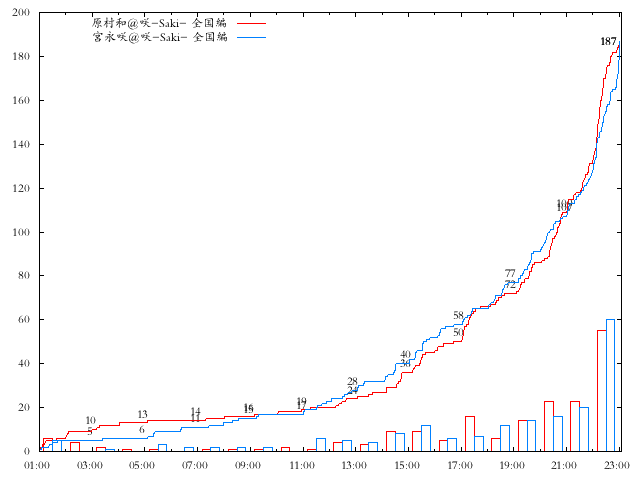
\includegraphics[width=\textwidth]{images/graph1223.png}
\end{minipage}}
% \end{wrapfigure}
\end{tabular}
\CTEXindent

终于迎来了 1223 的决赛。\uline{宫永咲}对\uline{原村和},正是\uwave{麻将}写出的最精彩的剧本。然而,这也是最后的矛盾。\uline{自由}厨\uline{咲},\uline{末原}厨\uline{和},于是这场给谁萌王,直到比赛最后都没有争执出来。由于\uline{自由}已经没有票力,所以整个海外相当于\uline{末原}一人把持厨\uline{和};而本土则是以\uline{まこ厨}为代表,表示既然运营不砍票了,就要在决赛努力刷\uline{咲}。海外\uline{和},本土\uline{咲},实质上是海外的碾压。但是这天发生了奇妙的事件,各种巧合造就了神奇的结果。

首先要说的是服务器被攻击的问题。看到\uwave{麻将}胜利会师,显然有人感到不满,于是用低劣的手段攻击了code发行所。遭到攻击的发行所,只有少数人能够领到票,大部分情况下都难以访问。攻击者试图以这种方式让\uwave{麻将}的票数变得难看,从而贬低这届萌王的价值。然而他的阴谋并没有得逞,海外技术不是吹的,本土也是兴奋于胜利会师一直在尝试取票——甚至一度在讨论如果发行所持续不可用的话,就废除code制。攻击者在中午暂停了攻击,比赛得以正常继续进行——所以大家可以看到上半赛段的票少得可怜——这都是攻击者耍的花招。攻击者在晚上发起了另一波攻击,但已经挡不住比赛的进行,效果不大。赛后,去年运营\uline{YUNE}和code发行屋\uline{OAa}出现,并告知这天的攻击主要来自4个中国的IP地址,攻击者不仅攻击了发行所190万余次,还尝试破解投票楼的管理员密码。至于究竟是谁干的,我想没有人会承认。

回到正常的比赛上,由于前些日子的比赛,萌文已经所剩无几。掌握票面生成器的\uline{自由}赛前和赛中完全没有出现,一度使群里产生了没有票面可用的危机感——于是各种手忙脚乱地手工准备萌文。\uline{自由}默默地向票面控制中心上传了准备好的五五开的票面,直到比赛开始前才被发现,各人终于松了一口气。然而这并不是结束,\uline{末原}又塞进去大量\uline{原村和}的票。还好由于发行所被攻击,票数并没有太多,\uline{和}领先\uline{咲}并不是很多。早上,本土\uwave{麻}起床,\uline{咲}取得了反超。发行所攻击停止,票数就又多了起来。

\uline{自由}和\uline{末原}为了各自的角色,两个人隔空在调度中心服务器掐起了架,你传上去我加上,你加上去我删掉,几来几回,票差也随着两人的掐架缠缠绵绵。\uline{自由}在贴吧发了个调查贴,调查在战吧\uline{宫永咲}和\uline{原村和}谁的人气更高——结果是\uline{宫永咲}更有人气。本土也在刷\uline{咲},也就保持了\uline{咲}的领先。晚上,\uline{末原}急了,暴走了一大波\uline{和}。\uline{自由}也急了,把票面中心的和票几乎删了个精光。\uline{末原}索性停止了挖掘机,不玩了。

海外\uwave{麻将}的撕逼大战暂时结束了,这就给了本土的机会。本土大量爆\uline{咲},在最后关头追上了\uline{和}。比赛马上结束,集计结果\uline{咲}胜\uline{和}一票,这可急死了\uline{和}厨。结果一刷新又出来一张\uline{和}的票,集计平票。在没有正式确认的情况下,谁也不敢说什么。终于比赛结果集计出来,187平票!

最终\uline{RUN}也没有出现,\uline{uBJ}在圣诞前夜,正式确定了决赛的平票,宣布了\uline{咲}\uline{和}双萌王的喜讯。

\chapter{结语}

2014日萌,以\uline{咲}\uline{和}平票双萌王的结果,为\uwave{圆}\uwave{麻}时代画上了圆满的句号。本届日萌,赛程最长,从七月中旬开始知道十二月底才宣告结束。细数这半年来的历程,不由得感慨万千。

\textbf{萌战即厨战},这是不可否认的事实,一味地粉饰太平反倒是对事实的不尊重。在多数人看来,多重是非正义的行为,然而不乏以多重违反规则为荣的人存在。对于比赛本身来说,多重是严重违反规则的错误行为,应该坚决打击。但应该看到,\textbf{多重是萌战的一部分},其他投票也是如此。单纯的散票比拼,如果没有很好的条件限制,有可能引入圈外的票源并导致圈内人的不满;提高投票的门槛,虽然有力缩小了圈子,但也限制了有价值的散票参与。另一方面,限制多重的手段越高超,散票的比例也就越小,少数技术能力强的人会主宰比赛,这就是厨。这会陷入一个不可解决的死胡同——越限制多重多重越多。辩证地来看,多重和散票是对立而统一的,萌战最好是通过平衡这两者来达成较为好看的比赛。日萌没有把握好这个平衡,从11年大寒波开始,又在多重审议的道路上陷入了泥潭,这就是多重泛滥、散票所剩无几的\uwave{圆}\uwave{麻}时代。\uwave{圆}\uwave{麻}时代的日萌真实,就是单一阵营或联盟把持萌战,打压其他阵营和驱逐散票的过程。
\\

参与这届厨战四个正好20岁的大学生,通过各种不同的手段和人脉,各自建立或延续成为了今年的四大阵营——\uwave{麻将}、\uwave{圆脸}、\uwave{电磁}、\uwave{LL}。多重票占据了今年的绝大部分,并从始至终控制着战场局势。

\begin{itemize}
\item 《{天才麻将少女}》——
\uwave{麻将}阵营是本届日萌的主角,虽然有着久远的历史,从09年就在萌战舞台上大展风姿,但却是完完全全的新厨团。从对萌战一无所知开始,在战场上摸爬滚打,自身努力加上天时地利人和,接连击溃\uwave{LL}、战胜\uwave{电磁}、反击\uwave{圆脸}、耗死\uline{运营},终于斩获历史最佳战绩。这么一个犹如少年漫画的励志故事,就是\uwave{麻将}这半年来所走过的路。Saki44和双萌王的神话,前无古人,后无来者。
\item 《{魔法少女小圆}》——
\uwave{圆脸}延续着13年的厨团组织,怀揣着要给\uline{晓美焰}八强的心态,最后结果算是无憾。\uwave{圆脸}在前期对\uwave{麻将}提供了相当大的帮助,最终结成神圣同盟,是阵营间友谊最好的体现。
\item 《{某科学的超电磁炮}》——
\uwave{电磁}则第一次成为了作品意义上的厨团,延续着世萌的厨团组织,为\uline{御坂美琴}的八强拼到了最后。虽然由于运营的砍票早早退场,但\uwave{炮}厨这种坚持到底的精神值得敬佩。
\item 《{Love Live!}》——
\uwave{LL}也是新建立的阵营,但有着萌战经验且成分较杂,与\uwave{电磁}关系密切。由于分组不利以及战略的失败,\uwave{LL}不断遭遇挫折,并和\uwave{麻将}逐渐交恶。由于战术的失败,最终导致了运营的砍票,遗憾退出比赛。\uwave{LL}是最难以评论的阵营,他们「自我中」的行为导致了日萌赛场上悲剧的结果。
% 但\uwave{LL}在新星萌和2015年度萌的表现却让人耳?目一新,也算是一种补偿。
\end{itemize}

\newpage

预选E04的\uwave{麻将}十连坐,正式拉开了厨战的序幕,\uwave{麻将}与\uwave{电磁}产生了最早的冲突。\uwave{电磁}登上舞台之后,统治日萌长达一个月。\uwave{电磁}的单一统治最终在0829第一次\uwave{电}\uwave{麻}大战,以\uline{爱宕洋榎}一票胜出\uline{茵蒂克丝}而告终,此后\uwave{麻将}与\uwave{电磁}达成了合作关系,在没有直接冲突的情况下合作到底。本战期间总共发生了三次\uwave{电}\uwave{麻}大战。\\
1011第二次\uwave{电}\uwave{麻}大战,即\uline{高鸭稳乃}对三\uwave{电磁}的一场,实际上是\uwave{圆}\uwave{麻}联盟对\uwave{电}\uwave{L}联合的关原合战,确定了\uwave{圆}\uwave{麻}联盟对\uwave{电}\uwave{L}联合的优势。\\
1023第三次\uwave{电}\uwave{麻}大战,\uline{宫永咲}胜出\uline{佐天泪子},同时连死隔壁\uline{南小鸟},\uwave{电磁}遭遇严重砍票。\\
\uwave{电磁}的最后一次出场,是1105的\uwave{圆}\uwave{麻}电三家混战,虽然\uline{御坂美琴}拿到了第一,却惨死于\uline{运营}的砍票。

以\uwave{圆}\uwave{麻}合作为主,海外四大阵营的相互连记,贯穿了砍票前的本战近乎两个月。整个本战期间,总共发生了十次\uwave{圆}\uwave{麻}合作、八次\uwave{电}\uwave{麻}合作,海外三连记发生了两次、四连记一次。海外大厨之间的和谐关系,可以说史上少见。这种大合作建立在各阵营的利益至上,虽然非常和谐,但也导致了大阵营联合绞死新番的产生。虽然\uwave{圆}\uwave{麻}最后留下来了几个新番组决,然而中间死掉的又不知有多少。

\uwave{麻}\uwave{拉}矛盾则在海外连记之下暗流涌动。\\
0819本战首日\uwave{麻将}遭到双杀和\uline{高坂穗乃果}的意外失利,以及0826\uline{矢泽妮可}和\uline{三千院凪}的败退,则造成了\uwave{麻将}与\uwave{LL}阵营之间最初的矛盾。\\
0912的\uline{西木野真姬}连记\uline{小木曾雪菜}直线逆转事件,使运营产生了砍票的想法。\\
0929\uline{天江衣}与\uline{园田海未}隔空对轰,则使两个阵营的矛盾显现了出来。虽然一定程度上两家还能保持着合作,但1012\uline{绚濑绘里}死于砍票之后,1015\uline{东条希}败于\uline{爱宕绢惠}则直接引爆了两家关系,最终爆发成今年唯一一起阵营间撕逼事件。\uwave{LL}角色遭到全数斩杀,只留下\uline{西木野真姬}进入组决,季后赛败给\uline{运营}的砍票。

\uwave{圆}\uwave{麻}联盟的十次合作,最终使\uwave{麻将}以32强占16的战绩,席卷了半壁江山。\uwave{圆脸}五色全数进入季后赛并保证了十六强席位。\uwave{圆}\uwave{麻}联盟是新时代的神圣同盟,清扫完对手把总账放到最后算。\\
1104\uline{宫永咲}对\uline{鹿目圆香},是赌上各自作品名誉的第一次\uwave{圆}\uwave{麻}大战。\\
1105的\uwave{圆}\uwave{麻}电三家混战,也是\uwave{麻将}的实票胜过\uwave{圆脸}。\\
比赛决定再开之后,十六进八的比赛也是\uwave{麻将}的实票碾压,这是第三次和第四次\uwave{圆}\uwave{麻}大战。\\
第五次\uwave{圆}\uwave{麻}大战也是最后一次\uwave{圆}\uwave{麻}大战,是1218八进四的\uline{宫永咲}对\uline{晓美焰}。\\
\uwave{圆}\uwave{麻}大战全部发生在季后赛和决胜赛圈,是「神圣同盟」性质的最佳表现。

值得一提的还有\uline{东山}阵营,主要是\uwave{麻将}阵营所领导的。进入本战的六个\uline{东山}角色,保送到32强的有五个:\uline{新子憧}、\uline{九条可怜}、\uline{由比滨结衣}、\uline{桐崎千棘}、\uline{中川花音},不亚于当年\uline{钉宫}阵营之威风。\uline{UMB}阵营则是\uwave{圆}\uwave{麻}联盟的副产物:\uline{高鸭稳乃}和\uline{鹿目圆香}都是阵营五大主力之一。

本届日萌的运营\uline{RUN},在测试了\uwave{舰娘}最萌之后,开始了今年的提名和比赛。\uline{RUN}在赛制上做了较大改动,比如二预的洪德法、三轮混战复活制、季后赛和交叉分组,希望能够限制住大阵营。\uline{RUN}曾以不正审议为由驱逐掉去年运营\uline{YUNE},但今年犯了更为严重的错误。针对\uwave{麻将}的强势,复活二回战时在投票版规制了「咲」这个字。\uline{RUN}在三回战开始时决定砍票,先后砍死\uwave{LL}和\uwave{电磁}阵营。最后在\uwave{圆}\uwave{麻}联手绞死\uwave{黄图}之后,为\uline{晓美焰}砍了个八强之后放弃治疗。比赛最后由\uline{uBJ}接手运营责任完成,并在圣诞前夜终于宣布结束。

code发行屋0907实行了(84)规制案后人间蒸发,多重变得肆无忌惮。1121的日本服务器查封案,从硬件环境上改变了日萌票源。决赛时发行所和投票版遭受攻击,赛后前发行屋\uline{OAa}和前运营\uline{YUNE}都出现并报告了这一行为。

本届日萌的多重技术上升到了一个新的高度,诞生了单人票力500的新一代海外技术厨。

本届因为砍票败退的角色有9位:\uline{绚濑绘里}、\uline{佐天泪子}、\uline{丹生谷森夏}、\uline{白井黑子}、\uline{大星淡}、\uline{西木野真姬}、\uline{御坂美琴}、\uline{宫永照}、\uline{清水谷龙华},其中\uwave{LL}2位、\uwave{电磁}3位、\uwave{麻将}3位;

由于砍票而晋级的角色有8位:\uline{爱丽丝·卡达列特}(2次)、\uline{松实宥}、\uline{香风智乃}、\uline{中川花音}、\uline{清水谷龙华}、\uline{佐仓杏子}、\uline{九条可怜}、\uline{晓美焰},其中\uwave{黄图}2位(3次)、\uwave{圆脸}2位、\uwave{麻将}2位。

本届日萌发行数上千的有6场:1105 「三家混战」 发行1545票,1011 「第二次\uwave{电}\uwave{麻}大战」 发行1328票,1023 「第三次\uwave{电}\uwave{麻}大战」 发行1194票,1218 「\uline{咲焰}相争」 发行1060票,1106 「季后赛」 发行1049票,0929 「隔空对轰」 发行1001票。
其中投票数上千的有3场:1105 「三家混战」 投出1441票,1011 「第二次\uwave{电}\uwave{麻}大战」 投出1139票,1218 「\uwave{咲焰}相争」 投出1021票。

萌王战有三场:0919\uline{鹿目圆香}(13日萌)胜出\uline{园城寺怜}(12日萌),1213\uline{园城寺怜}(12日萌)胜出\uline{巴麻美}(11日萌),1218\uline{宫永咲}(13度萌)胜出\uline{晓美焰}(14度萌)。

本届日萌有4次平票晋级:0725 E02组 \uline{佐仓杏子}、\uline{翠星石}、\uline{西木野真姬}、\uline{绚濑绘里} (82票),0731 Y07组 \uline{小路绫}、\uline{一条萤} (112票),0830 一回战 \uline{猪熊阳子}、\uline{姬柊雪菜} (123票),1223 决赛 \uline{宫永咲}、\uline{原村和} (187票)。
\\

2014日萌是\uwave{麻将}年,「\uwave{炮偶炮}、京\uline{钉}京、\uwave{圆}\uwave{麻}\uwave{圆}\uwave{麻}」代表着厨战的三个时代。02~04是日间动画统治的舞台;05~07宅向深夜动画来临,\uwave{魔炮}、\uwave{人偶}、\uwave{寒蝉}活跃,\uwave{管家}登上历史舞台;08~10是京都和\uline{钉宫}的战争,\uwave{麻将}登上历史舞台;11~14的现在则是\uwave{圆脸}和\uwave{麻将}的天下,也是\uwave{电磁}的征战史。\\
09、10两年,初生的\uwave{麻将}连续四强占二,没有萌王。\\
11年\uwave{炮姐}首轮胜\uwave{焰},却不幸遭遇发行所寒波,无缘八强;新阵营\uwave{圆脸}则四强占三,拿到第一个巨乳萌王\uline{学姐}。\\
12年\uwave{麻将}以\uwave{阿知贺篇}卷土重来,与\uline{钉宫}结盟完成八强占六,拿到首个萌王\uline{园城寺怜}。\\
13年\uwave{圆}\uwave{麻}首次同场竞技,\uwave{圆脸}遭遇海外围剿后怒而崛起,再次四强占三,\uwave{鹿目圆香}拿到首个复活萌王;\uwave{麻将}遭到砍票而退场,无缘16强。\\
14年\uwave{麻将}以全国篇与\uwave{圆脸}结成「神圣同盟」,最后发起复仇之战,四强占三,\uline{咲}\uline{和}平票双萌王。

\uwave{圆}\uwave{麻}时代的特征,在于单极阵营联盟的绝对统治。以11年发行所大寒波为标志,技术厨开始统治日萌。13年开始以限制多重为由的砍票,分别被\uwave{圆脸}和\uwave{麻将}抓住把柄最终称王。\uwave{圆}\uwave{麻}时代持续了四年,以\uwave{圆脸}2萌王、\uwave{麻将}3萌王结束。
\\

前事不忘,后事之师,谁又能预料到将来是怎样的场景,来怀念这个时代呢?

\begin{flushright}
 \zihao{4}\rm\kasho {王者自由}

 \kai 2014年12月31日
\end{flushright}

\chapter*{2014日萌大事表}
\addcontentsline{toc}{chapter}{2014日萌大事表}

{\zihao{6}\renewcommand\baselinestretch{1.25}\selectfont
\ctexset{space=true}
\begin{longtable}{rccccccc}
\hline
	\bf 日期 & \bf 场次 & \bf 比赛情况 & \bf \uwave{麻将}阵营 & \bf \uwave{圆}\uwave{麻}关系 & \bf \uwave{电}\uwave{麻}关系 & \bf \uwave{麻}\uwave{拉}关系\\ \hline
	7/13(日) & 一予抽選 & {\color{white}比赛情况比赛情况} & & & &\\ \hline
	7/19(土) & Y1組 & & & & &\\ \hline
	7/20(日) & Y2組 & & & & &\\ \hline
	7/21(祝) & Y3組 & & & & &\\ \hline
	7/22(火) & Y4組 & & & & &\\ \hline
	7/24(木) & E1組 & & & & &\\ \hline
	7/25(金) & E2組 & & & & &\\ \hline
	7/26(土) & E3組 & & & & &\\ \hline
	7/27(日) & E4組 & & \uwave{麻将}十连坐 & & &\\ \hline
	7/29(火) & Y5組 & & & & &\\ \hline
	7/30(水) & Y6組 & & & & &\\ \hline
	7/31(木) & Y7組 & & & & &\\ \hline
	8/1(金) & Y8組 & & & & &\\ \hline
	8/3(日) & E5組 & \uline{森夏}第一 \uline{炮憧}第二 & \uline{憧}Top失败 & & \uwave{电}\uwave{麻}小冲突之一 &\\ \hline
	8/4(月) & E6組 & & & & &\\ \hline
	8/6(水) & E7組 & & & & &\\ \hline
	8/7(木) & E8組 & & \uline{乳和}Top & & \uwave{电}\uwave{麻}小冲突之二 &\\ \hline
	8/10(日) & 二次予選 & \uwave{电磁}4个二预 & \uwave{麻将}4个二预 & & &\\ \hline
	8/13(水) & 本選抽選 & & Saki44 & & &\\ \hline
	8/19(火) & A,B,C,D 1-1 & \uline{果皇}败给\uline{团子} & \uline{卷饼}\uline{画板}遭双杀 & & & \uwave{麻}\uwave{拉}矛盾之始\\ \hline
	8/20(水) & A,B,C,D 1-2 & & & & &\\ \hline
	8/21(木) & A,B,C,D 1-3 & & & & &\\ \hline
	8/22(金) & A,B,C,D 1-4 & & & 第一次\uwave{圆}\uwave{麻}合作 & &\\ \hline
	8/23(土) & E,F,G,H 1-1 & & & & &\\ \hline
	8/24(日) & E,F,G,H 1-2 & 海外四连记 & & 第二次\uwave{圆}\uwave{麻}合作 & &\\ \hline
	8/26(火) & E,F,G,H 1-3 & \uline{妮可}\uline{三千}败给\uwave{电磁} & & & & 第一次\uwave{麻}\uwave{拉}矛盾\\ \hline
	8/27(水) & E,F,G,H 1-4 & & & & &\\ \hline
	8/28(木) & I,J,K,L 1-1 & & & & &\\ \hline
	8/29(金) & I,J,K,L 1-2 & & & 第三次\uwave{圆}\uwave{麻}合作 & 第一次\uwave{电}\uwave{麻}大战 &\\ \hline
	8/30(土) & I,J,K,L 1-3 & \uline{阳子}\uline{雪菜}平票 & & & &\\ \hline
	8/31(日) & I,J,K,L 1-4 & & & & &\\ \hline
	9/2(火) & M,N,O,P 1-1 & & & & &\\ \hline
	9/3(水) & M,N,O,P 1-2 & & & & &\\ \hline
	9/4(木) & M,N,O,P 1-3 & & & & 第一次\uwave{电}\uwave{麻}合作 &\\ \hline
	9/5(金) & M,N,O,P 1-4 & & & & &\\ \hline
	9/6(土) & Q,R,S,T 1-1 & & & 第〇次\uwave{圆}\uwave{麻}大战 & &\\ \hline
	9/7(日) & Q,R,S,T 1-2 & (84)规制案 & & & &\\ \hline
	9/9(火) & Q,R,S,T 1-3 & & & & 第二次\uwave{电}\uwave{麻}合作 &\\ \hline
	9/10(水) & Q,R,S,T 1-4 & & & & &\\ \hline
	9/11(木) & U,V,W,X 1-1 & & & & 第三次\uwave{电}\uwave{麻}合作 &\\ \hline
	9/12(金) & U,V,W,X 1-2 & \uline{真姬}\uline{雪菜}直线逆转 & & & & 第二次\uwave{麻}\uwave{拉}矛盾\\ \hline
	9/13(土) & U,V,W,X 1-3 & & & & &\\ \hline
	9/14(日) & U,V,W,X 1-4 & \uline{马达}伪票 & & 第四次\uwave{圆}\uwave{麻}合作 & &\\ \hline
	9/16(火) & 敗復1回戦 & \uline{加农}炮 & & & &\\ \hline
	9/19(金) & A2-1 C2-2 E2-1 & 海外三连记 & & 第五次\uwave{圆}\uwave{麻}合作 & & 第三次\uwave{麻}\uwave{拉}矛盾\\ \hline
	9/20(土) & A2-2 C2-1 E2-2 & & & & 第四次\uwave{电}\uwave{麻}合作 &\\ \hline
	9/21(日) & B2-1 D2-2 F2-1 & & & 第六次\uwave{圆}\uwave{麻}合作 & &\\ \hline
	9/22(月) & B2-2 D2-1 F2-2 & & & & &\\ \hline
	9/23(祝) & G2-2 I2-1 K2-2 & & & & 第五次\uwave{电}\uwave{麻}合作 &\\ \hline
 9/24(水) & G2-1 I2-2 K2-1 & & & & &\\ \hline
	9/26(金) & H2-2 J2-1 L2-2 & 海外三连记 & & 第七次\uwave{圆}\uwave{麻}合作 & 第六次\uwave{电}\uwave{麻}合作 &\\ \hline
	9/27(土) & H2-1 J2-2 L2-1 & & & & &\\ \hline
	9/28(日) & M2-1 O2-2 Q2-1 & 三\uwave{麻}连记 & & & &\\ \hline
	9/29(月) & M2-2 O2-1 Q2-2 & \uline{小衣}\uline{海未}隔空对轰 & & 第八次\uwave{圆}\uwave{麻}合作 & & 第四次\uwave{麻}\uwave{拉}矛盾\\ \hline
	9/30(火) & N2-1 P2-2 R2-1 & & & & &\\ \hline
	10/1(水) & N2-2 P2-1 R2-2 & & & & & \uwave{麻}\uwave{拉}短暂合作之一\\ \hline
	10/3(金) & S2-2 U2-1 W2-2 & & & & &\\ \hline
	10/4(土) & S2-1 U2-2 W2-1 & & & & & \uwave{麻}\uwave{拉}短暂合作之二\\ \hline
	10/5(日) & T2-2 V2-1 X2-2 & & & & 第七次\uwave{电}\uwave{麻}合作 &\\ \hline
	10/6(月) & T2-1 V2-2 X2-1 & & & & &\\ \hline
	10/8(水) & 敗復2回戦 & 晋级的\uline{马达} & NGword 咲 & & &\\ \hline
	10/11(土) & A3 G3 & \uwave{电}\uwave{麻}对轰 & \uline{稳乃}635票 & 第九次\uwave{圆}\uwave{麻}合作 & 第二次\uwave{电}\uwave{麻}大战 &\\ \hline
	10/12(日) & B3 H3 & \uline{绘里}死于砍票 & & & \uwave{电}\uwave{麻}小冲突之三 &\\ \hline
	10/13(祝) & C3 I3 & \uline{东}\uwave{圆}连记 & & & &\\ \hline
	10/14(火) & D3 J3 & & \uline{爱姐}婊\uline{受久} & & &\\ \hline
	10/15(水) & E3 K3 & & & & & 第五次\uwave{麻}\uwave{拉}矛盾\\ \hline
	10/16(木) & F3 L3 & & & & &\\ \hline
	10/18(土) & M3 S3 & \uline{苍星石}退场 & & & &\\ \hline
	10/19(日) & N3 T3 & & & & 第八次\uwave{电}\uwave{麻}合作 &\\ \hline
	10/20(月) & O3 U3 & & & & \uwave{电}\uwave{麻}小冲突之四 &\\ \hline
	10/21(火) & P3 V3 & & & & &\\ \hline
	10/22(水) & Q3 W3 & & & & &\\ \hline
	10/23(木) & R3 X3 & & & & 第三次\uwave{电}\uwave{麻}大战 &\\ \hline
	10/25(土) & 敗復3回戦 & \uwave{春物}复活 & & 第十次\uwave{圆}\uwave{麻}合作 & &\\ \hline
	10/28(火) & PlayOff抽選 & & 32占16 & & &\\ \hline
	10/30(木) & FL1 & & \uline{笨淡}死于砍票 & & &\\ \hline
	10/31(金) & FL2 & \uline{真姬}死于砍票 & & & &\\ \hline
	11/1(土) & FL3 & & & & &\\ \hline
	11/2(日) & FL4 & & & & &\\ \hline
	11/4(火) & FL5 & & & 第一次\uwave{圆}\uwave{麻}大战 & &\\ \hline
	11/5(水) & FL6 & \uline{炮姐}惨死砍票 & & 第二次\uwave{圆}\uwave{麻}大战 & 第四次\uwave{电}\uwave{麻}大战 &\\ \hline
	11/6(木) & FL7 & & \uline{照姐}死于砍票 & & &\\ \hline
	11/7(金) & FL8 & & & & &\\ \hline
	11/21(金) & & 服务器查封案 & & & &\\ \hline
	12/10(水) & 決勝T抽選 & 比赛决定再开 & 16占9 & & &\\ \hline
	12/13(土) & FT1,3,5,7 & & & 第三次\uwave{圆}\uwave{麻}大战 & &\\ \hline
	12/14(日) & FT2,4,6,8 & & & 第四次\uwave{圆}\uwave{麻}大战 & &\\ \hline
	12/17(水) & QF1 QF3 & & \uline{和玄稳怜} & & &\\ \hline
	12/18(木) & QF2 QF4 & & \uline{咲} & 第五次\uwave{圆}\uwave{麻}大战 & &\\ \hline
	12/21(日) & SF1 SF2 & & \uline{咲}\uline{和}\uline{稳} & & &\\ \hline
	12/23(日) & Final & 发行所遭攻击 & \uline{咲}\uline{和}平票 & & & \\ \hline
\end{longtable}
}
